\documentclass[12pt,a4paper]{article}
%-------------------------------------------
%---Packages--------------------------------
%-------------------------------------------
\usepackage[utf8]{inputenc}
%\usepackage[T1]{fontenc}
%\usepackage{txfonts}
\usepackage{amsmath}
\usepackage{amsthm}
\usepackage{amsfonts}
\usepackage{array}
\usepackage{amssymb}
\usepackage{blindtext}
\usepackage{caption}
\usepackage{color}
\usepackage{csquotes}	    %
\usepackage{enumitem}	    %pour mieux bosser avec les listes. ajoute option label
\usepackage[yyyymmdd]{datetime}        %pour définir date custom
\usepackage{etaremune}
\usepackage{environ}
\usepackage{fancybox}
\usepackage{fancyhdr} 	    % Custom headers and footers
\usepackage{fancyref}
%\usepackage{float}
\usepackage{floatrow}       %float and floatrow can't be together...
\usepackage{gensymb}
\usepackage{graphicx}
\usepackage[colorlinks=true, linkcolor=purple, citecolor=cyan]{hyperref}
\usepackage{footnotebackref}
\usepackage{lipsum}
\usepackage{mathtools}
\usepackage{multicol}	    %gérer plusieurs colonnes
\usepackage{setspace}
\usepackage{subcaption}
\usepackage{todonotes}	    %Bonne gestion des TODOs
%TODO commenté pour tester l'utilité... à voir% \usepackage[tc]{titlepic}      %Permet de mettre une image en page de garde
\usepackage{tikz}	    % Pour outil de dessin puissant
\usepackage{ulem}	    %underline sur plusieurs lignes (avec \uline{})
\usepackage{vmargin} 	    %gestion des marges, avec dans l'ordre : gauche, haut, droit, bas, en-tête, entre en-tête et texte, bas de page, hauteur entre bas de page et texte
\usepackage{wrapfig}
\usepackage{xcolor}
\usepackage{xparse}                    %Pour utiliser NewDocumentCommand et des arguments 'mmooo'
%\usepackage{fullpage} 	    %supprime toutes les marges allouées aux notes, aussi en haut et en bas

%\ExplSyntaxOn
\pagestyle{fancyplain}	    %Makes all pages in the document conform to the custom headers and footers

%-------------------------------------------
%---Document Commands-----------------------
%---------------------------{----------------
\NewDocumentCommand{\framecolorbox}{oommm}
 {% #1 = width (optional)
  % #2 = inner alignment (optional)
  % #3 = frame color
  % #4 = background color
  % #5 = text
  \IfValueTF{#1}%
   {\IfValueTF{#2}%
    {\fcolorbox{#3}{#4}{\makebox[#1][#2]{#5}}}%
    {\fcolorbox{#3}{#4}{\makebox[#1]{#5}}}%
   }%
   {\fcolorbox{#3}{#4}{#5}}%
 }%
%------------------------------------------------
%------------------ENGLISH----------------------
%----------------------------------------------

\NewDocumentCommand{\epflTitle}{mO{Olivier Cloux}O{\today}O{Notes de Cours en}D<>{../../Common}}%Arguments : Matière, Auteur, Date, Titre du doc
{
\begin{titlepage}
    \vspace*{\fill}
    \begin{center}
        \normalfont \normalsize
        \textsc{Ecole Polytechnique Fédérale de Lausanne} \\ [25pt] % Your university, school and/or department name(s)
        \textsc{#4} %Titre du doc
        \\ [0.4 pt]
        \horrule{0.5pt} \\[0.4cm] % Thin top horizontal rule
        \huge #1 \\ % Matière
        \horrule{2pt} \\[0.5cm] % Thick bottom horizontal rule
        
\includegraphics[width=8cm]{#5/EPFL_logo}
        ~\\[0.5 cm]
        \small\textsc{#2}\\[0.4cm]
        \small\textsc{#3}\\
        ~\\
        ~\\
        
\includegraphics[scale=0.5]{#5/creativeCommons}
    \end{center}
    \vspace*{\fill}
\end{titlepage}
}


%-------------------------------------------
%-------------MATH NEW COMMANDS-------------
%-------------------------------------------
\newcommand{\somme}[2]{\ensuremath{\sum\limits_{#2}^{#1}}}
\newcommand{\produit}[2]{\ensuremath{\prod\limits_{#2}^{#1}}}
\newcommand{\limite}{\lim\limits_}
\newcommand{\llimite}[3]{\limite{\substack{#1 \\ #2}}\left(#3\right)}	%limites à deux condiitons
\newcommand{\et}{\mbox{ et }}
\newcommand{\deriv}[1]{\ensuremath{\, \mathrm d #1}}	%sigle dx, dt,dy... des dérivées/intégrales
%\newcommand{\fx}{\ensuremath{f'(\textbf{x}_0 + h}}
\newcommand{\ninf}{\ensuremath{n \to \infty}}	       %pour les limites : n tend vers l'infini
\newcommand{\xinf}{\ensuremath{x \to \infty}}	       %pour les limites : x tend vers l'infini
\newcommand{\infint}{\ensuremath{\int_{-\infty}^{\infty}}}
\newcommand{\xo}{\ensuremath{x \to 0}}									%x to 0
\newcommand{\no}{\ensuremath{n \to 0}}									%n zéro
\newcommand{\xx}{\ensuremath{x \to x}}									%x to x
\newcommand{\Xo}{\ensuremath{x_0}}										%x zéro
\newcommand{\X}{\ensuremath{\mathbf{X}} }
\newcommand{\A}{\ensuremath{\mathbf{A}} }
\newcommand{\R}{\ensuremath{\mathbb{R}} }								%ensemble de R
\newcommand{\rn}{\ensuremath{\mathbb{R}^n} } 							%ensemble de R de taille n
\newcommand{\Rm}{\ensuremath{\mathbb{R}^m} }  							%ensemble de R de taille m
\newcommand{\C}{\ensuremath{\mathbb{C}} }
\newcommand{\N}{\ensuremath{\mathbb{N}} }
\newcommand{\Z}{\ensuremath{\mathbb{Z}} }
\newcommand{\Q}{\ensuremath{\mathbb{Q}} }
\newcommand{\rtor}{\ensuremath{\R \to \R} }
\newcommand{\pour}{\mbox{ pour }}
\newcommand{\coss}[1]{\ensuremath{\cos\(#1\)}}						%cosinus avec des parenthèses de bonne taille (genre frac)
\newcommand{\sinn}[1]{\ensuremath{\sin\(#1\)}}					%sinus avec des parentèses de bonne taille (genre frac)
\newcommand{\txtfrac}[2]{\ensuremath{\frac{\text{#1}}{\text{#2}}}}		%Fractions composées de texte
\newcommand{\evalfrac}[3]{\ensuremath{\left.\frac{#1}{#2}\right|_{#3}}}
\renewcommand{\(}{\left(}												%Parenthèse gauche de taille adaptive
\renewcommand{\)}{\right)}
\newcommand{\longeq}{=\joinrel=}												%Parenthèse droite de taille adaptive


%-------------------------------------------------------
%------------------MISC NEW COMMANDS--------------------
%-------------------------------------------------------
\newcommand{\degre}{\ensuremath{^\circ}}
%\newdateformat{\eudate}{\THEYEAR-\twodigit{\THEMONTH}-\twodigit{\THEDAY}}



%-------------------------------------------------------
%------------------TEXT NEW COMMANDS--------------------
%-------------------------------------------------------
\newcommand{\ts}{\textsuperscript}
\newcommand{\evid}[1]{\textbf{\uline{#1}}}        %mise en évidence (gras + souligné)



%\newcommand{\Exemple}{\underline{Exemple}}
\newcommand{\Theoreme}{\underline{Théorème}}
\newcommand{\Remarque}{\underline{Remarque}}
\newcommand{\Definition}{\underline{Définition} }
\newcommand{\skinf}{\sum^{\infty}_{k=0}}
\newcommand{\combi}[2]{\ensuremath{\begin{pmatrix} #1 \\ #2 \end{pmatrix}}}	%combinaison parmi 1 de 2
\newcommand{\intx}[3]{\ensuremath{\int_{#1}^{#2} #3 \deriv{x}}}				%intégrale dx
\newcommand{\intt}[3]{\ensuremath{\int_{#1}^{#2} #3 \deriv{t}}}				%intégrale dy
\newcommand{\misenforme}{\begin{center} Mis en forme jusqu'ici\\ \line(1,0){400}\\ normalement juste, mais à améliorer depuis ici\end{center}}	%raccourci pour mise en forme
\newcommand*\circled[1]{\tikz[baseline=(char.base)]{
            \node[shape=circle,draw,inner sep=1pt] (char) {#1};}}			%pour entourer un chiffre
\newcommand{\horrule}[1]{\rule{\linewidth}{#1}} 				% Create horizontal rule command with 1 argument of height

\theoremstyle{definition}
\newtheorem{exemp}{Exemple}
\newtheorem{examp}{Example}


%-------------------------------------------
%---Environments----------------------------
%-------------------------------------------
\NewEnviron{boite}[1][0.9]{%
	\begin{center}
		\framecolorbox{red}{white}{%
			\begin{minipage}{#1\textwidth}
 	 			\BODY
			\end{minipage}
		}
	\end{center}
}
\NewEnviron{blackbox}[1][0.9]{%
	\begin{center}
		\framecolorbox{black}{white}{%
			\begin{minipage}{#1\textwidth}
 	 			\BODY
			\end{minipage}
		}
	\end{center}
}
\NewEnviron{exemple}[1][0.8]{%
    \begin{center}
        \framecolorbox{white}{gray!20}{%
            \begin{minipage}{#1\textwidth}
                \begin{exemp}
                    \BODY
                \end{exemp}
            \end{minipage}
        }
    \end{center}
}
\NewEnviron{suiteExemple}[1][0.8]{%
    \begin{center}
        \framecolorbox{white}{gray!20}{%
            \begin{minipage}{#1\textwidth}
                \BODY
            \end{minipage}
        }
    \end{center}
}
\NewEnviron{colExemple}[1][0.8]{%
    \begin{center}
        \framecolorbox{white}{gray!20}{%
            \begin{minipage}{#1\columnwidth}
                \begin{exemp}
                    \BODY
                \end{exemp}
            \end{minipage}
        }
    \end{center}
}
\NewEnviron{example}[1][0.8]{%
    \begin{center}
        \framecolorbox{white}{gray!20}{%
            \begin{minipage}{#1\textwidth}
                \begin{examp}
                    \BODY
                \end{examp}
            \end{minipage}
	}
    \end{center}
}
\NewEnviron{systeq}[1][l]{
			\begin{center}
				$\left\{\begin{array}{#1}
					\BODY
				\end{array}\right.$
			\end{center}
 }





%-------------------------------------------
%---General settings-----------------------
%-------------------------------------------
\renewcommand{\headrulewidth}{1pt}										%ligne au haut de chaque page
\renewcommand{\footrulewidth}{1pt}										%ligne au pied de chaque page
\setstretch{1.6}
\author{Olivier Cloux}

\usepackage[tc]{titlepic}
\usepackage{graphicx}
\usepackage{blindtext}
%\usepackage[a4paper]{geometry}
\setcounter{section}{-1}
\date{Printemps 2015}
\title{	
\normalfont \normalsize 
\textsc{Ecole Polytechnique Fédérale de Lausanne} \\ [25pt] % Your university, school and/or department name(s)
\textsc{Note de cours en }\\ [0pt] %Name of the course
\horrule{0.5pt} \\[0.4cm] % Thin top horizontal rule
\huge Analyse II\\ % The assignment title<
\horrule{2pt} \\[0.5cm] % Thick bottom horizontal rule

\includegraphics[width=8cm]{images/EPFL_logo}}
\renewcommand{\contentsname}{Table des Matières}
\begin{document}
\setstretch{1}
\maketitle
\newpage
\tableofcontents
\setstretch{1.6}
\section*{Préambule}
Pour Moodle : nom : Analyse II, clé : \underline{2015AnalyseII-MATH-106(e)}\\
Salle : CO016. Séries mises en ligne le lundi, correction le lundi suivant.
\section{Équations différentielles}
\evid{Répéter :} 
\begin{enumerate}
	\item Méthode d'intégration
	\item Fonctions de classe $C^n$
	\item restriction d'une fonction
\end{enumerate}
\evid{Motivation} physique, économie, biologie,...\\
\evid{Appellation :} equation différentielle (ordinaire) = ED / EDO (ODE en anglais)

\subsection{Introduction, motivation, exemples}
Une EDO  c'est quoi ?  C'est une expression de la forme 
\begin{equation}
	E\(x,y(x),y'(x),...,y^{(n)}(x)\) = 0
	\label{ed_long}
\end{equation}
où E est une fonction donnée, E :  $\R^{n+2} \to$ \R pour $n\in \N^*$. On cherche un intervalle $I = ]a,b[\ ,\ a < b$, et une fonction $y : I \to \R$ de classe $C^{n}$, de sorte que ~\eqref{ed_long} soit satisfaite pour tout $x\in I$\\
\begin{boite}
	\evid{Remarque :} Souvent, pour simplifier la notation on écrit
	\begin{equation}
		E(x,y,y',y'',...,y^{n}) = 0
		\label{ed_court}
	\end{equation}
	au lieu de ~\eqref{ed_long}
\end{boite}
\begin{boite}
	\evid{Remarque} L'expression ``ordinaire'' veut dire que la fonction recherchée est une fonction \underline{d'une seule variable réelle} (Des équations aux dérivées partielles EDP (ou PDE en anglais) font intervenir des fonctions inconnues de plusieurs variables)
\end{boite}
\begin{boite}
	\evid{Définition} Si dans ~\eqref{ed_court} E est une fonction non-constante de $y^{(n)}$ E \enquote{dépend} de $y^{n}$ on dit que l'équation est \underline{d'ordre} n 
\end{boite}
\begin{boite}
	\evid{Définition} Si dans ~\eqref{ed_court} E est une fonction polynôme de $y^{(n)}$ de degré d, alors on dit que l'ED est de degré d
\end{boite}
\begin{boite}
	\evid{Définition} Si dans ~\eqref{ed_court} E est une fonction constante de x (E ne dépend pas de x), l'équation différentielle est dite ``autonome''
\end{boite}
\evid{Exemples :}\\
\begin{tabular}{ll}
$y = 0$ & pas une ED\\
$y'=0$ & n=1 (=ordre)\\
		& d=1 (=degré)\\
		&autonome\\
$\sin(y') = 0$ & n=1 (=ordre)\\
	&degré pas défini\\
	&autonome\\
$\sin(x)y'-\sin(y) = 0$ & n=1 (=ordre)\\
	&d=1 (=degré)\\
$y''y' +  \sin(y') = 0$ &  n=2\\
	&d=1\\
	&autonome\\
$y'''+y''+y' + \sin(x) = 0$ & n=3\\
	&d=1\\
$\sin(x)(y')^2 + y = 0$ & n=1, d=2
\end{tabular}\\
\evid{Exemples de solutions}\\
\begin{tabular}{ll}
	$y' = 0$ & Solution : $y(x) = C, x\in \R, \forall C \in R$\\
	$y'-1 = 0$ & Solution : $y(x) = x + C, x\in \R, \forall C \in \R$\\
	$y'-e^x = 0 \iff y'(x) = e^x$ & Solution $y(x) = e^x + C, x\in \R,\forall C \in  \R$\\
	$y'-f(x) = 0 \iff y' = f(x)$ & Solution $y(x) = F(x) + C$ sur $]a,b[$ (domaine ou f est continue), $\forall C \in \R$
\end{tabular}
voir aussi Série, échauffement.\\
\begin{boite}
	\evid{A propos Série 1} ``Typologie'' des équations, les solutions sont données, vérifier que les solutions données satisfont les équations.
\end{boite}
\begin{boite}
	\evid{Remarque} Soit y une solution d'une ED sur l'intervalle $I = ]a,b[$. Soit $]c,d[ \subset ]a,b[$. Alors la restriction de la fonction y à l'intervalle $]c,d[$ est aussi une solution.
\end{boite}
\begin{boite}
	\evid{Définition} On dit qu'une solution est \underline{maximale}, si elle n'est pas la restriction d'une autre solution.
\end{boite}
\begin{boite}
	\evid{Définition} La \underline{Solution générale} d'une ED est l'ensemble de toutes les solutions de l'équation. Résoudre une ED revient à trouver la solution générale
\end{boite}
\setlength{\columnseprule}{0.05cm}
\begin{multicols}{3}
	\evid{Plus d'exemples}
	A : $y' = y$\\
	B : $y' = -y$\\
	C : $y'' = y$\\
	D : $y'' = -y$\\
	E : $y' = y+1$\\
	F : $y' = -xy$\\ 
	G$y'+ \frac{1}{x}y = 0, x \in  \R^*$\\
\end{multicols}

\evid{Solutions} Dans ce qui suit, $y : \R \to \R$, sauf si indiqué autrement, $C,C_1,C_2 \in \R$\\
$\begin{array}{lll}
\text{A: }& &y(x) = Ce^x : y'(x) =Ce^x = y(x)\\
\text{B: }& &y(x) = Ce^{-x} : y'(x) = -Ce^{-x} = -y(x)\\
\text{C: }& &y(x) = C_1e^x + C_2e^{-x} \text{(ED d'ordre 2)} =C_1\cosh(x) + C_2\sinh(x)\\
\text{D: }& &y(x) = C_1\sin(x) + C_2\cos(x)\\
	&	&y'(x) = C_1\cos(x) -C_2\sin(x)\\
	&	&y''(x) = -C_1\sin(x) - C_2\cos(x) =-(C_1\sin(x) + C_2\cos(x)) = -y(x)\\
\text{E: }& & y(x) = Ce^x -1\\
	&	&y'(x) = Ce^x = y(x) + 1\\
\text{F: }& & y(x) = Ce^{-\frac{1}{2}x^2}\\
\text{G: }& & y(x) = \frac{C}{x}\\
	&	&y'(x) = -\frac{C}{x^2} = -\frac{1}{x}y(x)

\end{array}$

\underline{Solution générale (pour G)}\\
$\{y(x) = \frac{C}{x}, x \in ]0,\infty[, C \in \R$\\
$y(x) = \frac{C}{x}, x\in ]-\infty,0[, C\in\R\}$\\
\begin{boite}
	\evid{Convention (exercices)}La solution générale doit être donnée par l'équation donnée sans réécriture. Voir la fin du chapitre 0 pour une explication
\end{boite}
\begin{boite}
	\evid{Remarque} (dépend du paramètre) Si $y(x)$ est solution d'une équation autonome par $x\in \R$, alors $y_c(x) : y(x+C)$ est aussi solution pour tout $C \in \R$ (vérifier)
\end{boite}
\begin{boite}
	\evid{Constat} La solution d'une ED d'ordre n n'est typiquement pas unique. Elle dépend typiquement de n paramètres. Des solutions \enquote{isolées} additionnelles sont possibles. 
\end{boite}

\subsubsection{Problème de Cauchy ou problème à condition initiale}
\evid{Exemple 1:}\\
$\underbrace{\underbrace{y' = y}_{ED}\quad , \quad \underbrace{y(0) = 1}_{CI}}_{\text{problème de Cauchy}}$. Solution générale : $y(x) = Ce^x, x \in \R, \forall C \in \R$.\\
La solution qui satisfait $y(0) = 1$ est celle avec $C = 1$, \\car $y(0) = Ce^0 = C = 1$\\
\\
\evid{Exemple 2:}\\
\begin{equation*}
	\underbrace{\underbrace{y'' = -y}_{ED} \quad , \quad\underbrace{y(0)= 1, y'(0) =0}_{CI}}_{\text{Problème de Cauchy}}
\end{equation*}
Solution générale : $y(x) = C_1\sin(x) + C_2\cos(x)\qquad  \ x \in \R \ , C_1, C_2 \in \R$\\
En évaluant $x$ en 0 (selon les CI), on peut trouver une première constante: $y(0) = C_2 = 1$\\
On prend ensuite la dérivée, afin de pouvoir examiner avec la seconde CI
\begin{equation*}
	y'(x) = C_1\cos(x) - C_2\sin(x)
\end{equation*}
Que l'on évalue à nouveau selon l'autre CI, afin de trouver la seconde constante :
$y'(0) = C_1 = 0$\\
La solution du problème de Cauchy est $y(x) = \cos(x), \ x\in\R$
\begin{boite}
	\underline{Attention!} Selon le type de l'ED, une condition initiale ne suffit pas pour sélectionner une solution unique
\end{boite}

\subsection{Équation différentielles du premier ordre}
Une ED est du premier ordre si elle est du type : $E(x,y,y') = 0$ (seulement une dérivée).

\subsubsection{Séparation des variables}
Une ED est dite à variables séparées, si on peut l'écrire sous la forme 
\begin{equation}
	E(x,y,y') = f(x) - g(y)y' = 0
	\label{eq_var_sep}
\end{equation}
Pour certaines fonctions $f$ et $g$\\
\evid{Résolution de l'équation}\\
Soit F une primitive de f et G une primitive de G. Alors toute fonction $y : ]a,b[ \to \R$ de classe $C^1 \ (]a,b[)$ qui satisfait
\begin{equation}
	F(x) - G(y(x)) = C \qquad \qquad x\in ]a,b[
	\label{res_eq_var_sep}
\end{equation}
est une solution de l'ED~\eqref{eq_var_sep}\\
\evid{Vérification :} On dérive ~\eqref{res_eq_var_sep} afin de vérifier : $\frac{d~\eqref{res_eq_var_sep}}{dx}:\\
 F'(x) - G'\Big(y(x)\Big)y'(x) = 0$ et donc on a $f(x) - g(y(x))y'(x) = 0$ puisque $F' = f,\ G'=g$ par définition de F et G
\begin{boite}
	\evid{Remarque} Donnée une solution sous forme \underline{implicite} \big(on a une équation pour $y(x)$\big), il faut encore (si possible) résoudre~\eqref{res_eq_var_sep} pour $y(x)$ pour obtenir la (les) solution(s) sous forme \underline{explicite}.
\end{boite}
${}$\\
\evid{Procédé de résolution pratique (recette de cuisine)}\\
On écrit $y' = \frac{dy}{dx}$ que l'on manipule comme une fraction de \enquote{$dy$} sur \enquote{$dx$}. On a pour~\eqref{eq_var_sep}\\
$\begin{array}{ll}
	f(x) - g(y)\frac{\deriv{y}}{\deriv{x}} = 0 & |\cdot \deriv{x}\\	
	f(x)\deriv{x} = g(y)\deriv{y}  &|\cdot \int \\
	\int f(x) \deriv{x} = \int g(y) \deriv{y} + C & \leftarrow \text{Ici on traite $y$ comme une variable}\\
	F(x) = G(y) + C & \leftarrow \text{Ici $y$ est une fonction de x}
\end{array}$\\
\evid{Exemple 1}\\
$\begin{array}{rll}
	\fcolorbox{red}{white}{$y'(x) = y$} &\to \frac{\deriv{y}}{\deriv{x}} = y \iff \frac{1}{y}\deriv{y} = \deriv{x}&\\ 
	&\to \int\frac{1}{y}\deriv{y}  = \int1\deriv{x} +C & C\in \R\\
	&\to\ln(|y|) = x+C & C\in \R\\
	&\to |y(x)| = e^{x+C} = e^C\cdot e^x & C\in\R\\
	&\to |y(x)| = Ce^x & C > 0,\ x\in \R\\
	e^C = C \text{ car constante}&\to y(x) = \pm Ce^x & C>0,\ x\in\R\\
	&\to y(x) = Ce^x  & C\in\R\setminus\{0\},\ x\in\R\\
\end{array}$\\
Il manque la solution $y(x) = 0,\ x\in\R$. Donc la solution générale est \underline{$y(x) = C\cdot e^x,\ x\in \R, \ C\in \R$}\\
\\
\evid{Exemple 2}\\
Soit l'ED \framecolorbox{red}{white}{$y'=y^2$}. Déterminer :
\begin{enumerate}[label=\alph*)]
	\item La solution générale
	\item La \underline{solution maximale} qui satisfait la CI $y(0) = y_0\in \R$, avec $y_0$ donné
\end{enumerate}
Pour la résolution, on utilise la recette de cuisine :
\begin{enumerate}[label=\alph*)]
	\item $y(x) = 0,\ x\in \R$ est une solution. Pour $y\neq 0$, l'ED est séparable :\\
	$\frac{\deriv{y}}{\deriv{x}} = y^2 \underset{y\neq 0}{\to} \frac{\deriv{y}}{y^2} = \deriv{x} \to \frac{-1}{y} = x+C\qquad C\in \R$\\
	$\to y(x) = \frac{-1}{x+C}\footnote{Attention, pas défini en x = -C. C'est l'autre solution à trouver}$\\
	La solution générale (maximale) est :\\
	$\left\{\begin{array}{rll}
	&y(x) = 0 & x\in \R\\
	\circled{1} & y(x) = \frac{-1}{x+C} & x\in ]-\infty,\ -C[ \ , \ C\in \R\\
	\circled{2} & y(x) = \frac{-1}{x+C} & x\in ]-C,\infty[ \  , \ C\in\R
	\end{array}\right\}$
\end{enumerate}
\begin{center}
	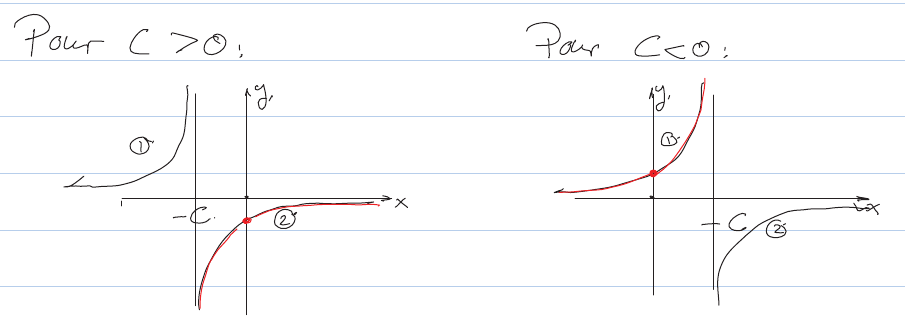
\includegraphics[scale=0.55]{images/sol1}
\end{center}
\leavevmode\\
\begin{enumerate}[label=\alph*), resume]
	\item \underline{Utilisation de la CI $y(0) = y_0$, avec $y_0 \in \R$ donné :}\\
		On a $y(0) = \frac{-1}{C}$ (dans 1 et 2), et donc $C = -\frac{1}{y_0}$, ce qui donne \\
		$y(x) = \frac{-1}{x-\frac{1}{y_0}} = \frac{y_0}{1-xy_0}$ (cas 1 et 2)\\
		La solution maximale avec CI $y(0) = y_0$ est donc \\
		$\begin{array}{llr}
		 	y(x) = 0  & ,x\in \R &$ si $y_0 = 0\\
			 y(x) = \frac{y_0}{1-xy_0} & ,x\in ]-\infty,\frac{1}{y_0}[&$ si $y_0 > 0\\
			 &&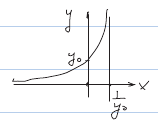
\includegraphics[scale=0.7]{images/y_geq_0}\\
			 y(x) = \frac{y_0}{1-xy_0} & ,x\in ]\frac{1}{y_0},\infty[&$ si $y_0 < 0\\ 
			 &&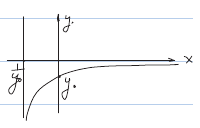
\includegraphics[scale=0.7]{images/y_leq_0}
		\end{array}$
\end{enumerate}
\leavevmode\\
\evid{Exemple 3}\\
Soit l'ED \framecolorbox{red}{white}{$2y^3 + 3xy^2y' = 0$}. À discuter le problème de Cauchy pour les CI $y(1) = 2,\ y(1) = -2,\ y(-1) = 2,\ y(0) = 0$
\begin{enumerate}[label=\alph*)]
	\item \evid{Solution générale}\\
			$y(x) = 0 \ , \ x\in\R$ est une solution. Après séparation des variables : \\
			$\begin{array}{lr}
			2y^3+3xy^2\frac{dy}{dx} = 0 \underset{\substack{y\neq 0 \\ x\neq 0}}{\iff} 3\frac{dy}{y} = -2\frac{dx}{x} & |\int\\
			\to 3\ln(|y|) = -2\ln(|x|) + \underbrace{\ln(C)}_{\in\R}  & C > 0\\
			\to\ln(|y|^3) = \ln(\frac{C}{|x|^2}) \to |y(x)|^3 = \frac{C}{|x|^2}  & C > 0\\
			\to|y(x)| = \frac{C}{|x|^{\frac{2}{3}}}  & C>0\\
			\to y(x) = \pm \frac{C}{|x|^{\frac{2}{3}}} & C>0\\
			\to y(x) = \frac{C}{|x|^{\frac{2}{3}}} & C \in \R\setminus\{0\}\\
			\end{array}$
		
			La solution générale est\\
			$\left\{\begin{array}{rlr}
				&y(x) = 0 & x\in \R\\
				\circled{1} & y(x) = \frac{C}{x^{\frac{2}{3}}} & x\in ]0,\infty[,\ C\in\R^*\\
				\circled{2} & y(x) = \frac{C}{(-x)^{\frac{2}{3}}} & x\in ]-\infty,\ 0 [,C\in\R^*
			\end{array}\)\}$\\
	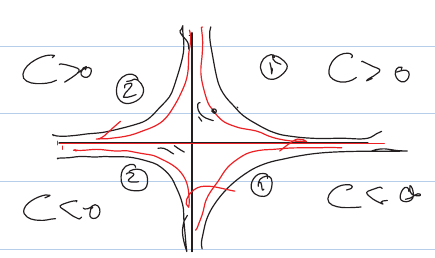
\includegraphics[scale=0.7]{images/sol_gen_ex_3}
	\item \evid{Solution des problèmes de Cauchy}\\
			\underline{Problème 1 :} $y(1) = 2$. On prend 1 : $y(1) =  \frac{C}{1^{\frac{2}{3}}} = 2 \to C = 2$, donc $y(x) = \frac{2}{x^{\frac{2}{3}}},\ x\in]0,\infty[$ (solution maximale)
			
			\underline{Problème 2 :} $y(1) = -2$. On prend 1 : $y(1) = \frac{C}{1} = -2 \to C = -2$, donc $y(x) = \frac{-2}{x^{\frac{2}{3}}},\ x\in]0,\infty[$ (solution maximale)
			
			\underline{Problème 3 :} $y(-1) = 2$. On prend 2 : $y(-1) = \frac{C}{(-(-1))^{\frac{2}{3}}} = C = 2$ donc $y(x) = \frac{2}{(-x)^{\frac{2}{3}}},\ x\in ]-\infty,0[$ (solution maximale)
			
			\underline{Problème 4 :} La solution est $y(x) = 0, \ x\in\R$ (solution maximale)
\end{enumerate}

\subsubsection{Applications}
\begin{itemize}
	\item modélisation de populations
	\item modélisation de certaines situations économiques
\end{itemize}
$y(t) \in \R$ la quantité d'argent / la taille d'une population / quantité de $CO_2$ dans l'atmosphère. On considérera $t \geq 0$ le temps.\\
Supposons que $y' = k\cdot y \ , \ y(0) = y_0 > 0$.\\
Soit y(t) la solution du problème de Cauchy\\
Alors $y(t + \delta)\footnote{$\delta$ petit $>0$} = y(t) + \underbrace{y'(t)\delta}_{k\delta y(t)} + o(\delta),\quad \delta \to 0$ \\
Donc $y(t+\delta) - y(t) = k\delta y(t) + o(\delta),\quad \delta \to 0$, ce qui nous montre que la croissance de la population est proportionnelle à la taille de la population.\\
Interprétation : $k > 0$ On a un accroissement proportionnel à $y(t)$ (on peut penser au pourcentage d'un taux d'intérêt d'une banque)\\
$k < 0$ On a un décroissement proportionnel à $y(t)$.\\
Solution : $y(t) = y_0e^{kt} \qquad ,t\geq 0$ (croissance exponentielle) (exemple 1, 0.2.1)\\
A comparer avec la solution de $y' = y^{2}, y(0) = y_0 > 0\footnote{Croissance plus vite que linéaire}$ \\%attention footnote
Solution : $y(t) = \frac{y_0}{1-y_0t}, t\in [0,\frac{1}{y_0}[$\\
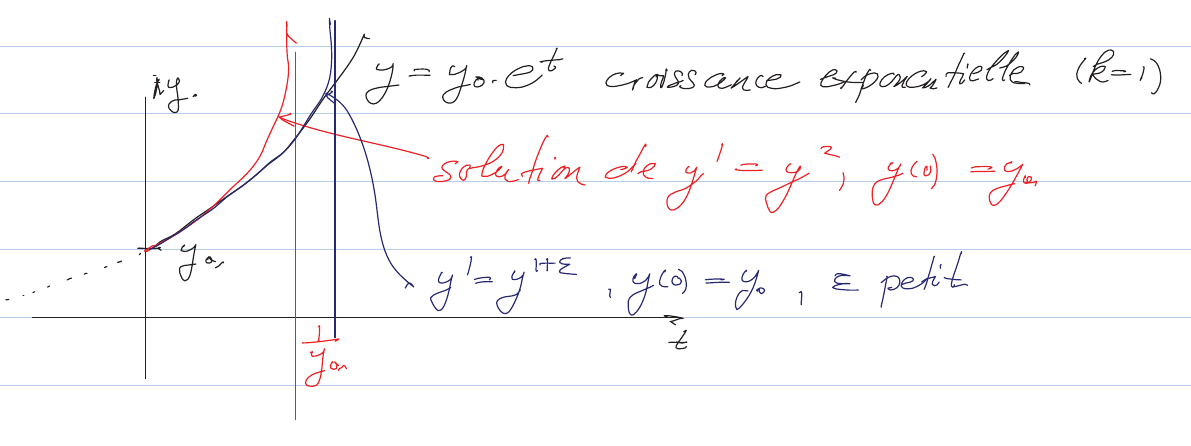
\includegraphics[scale=0.5]{images/croiss_expo}

\subsubsection*{Lois de croissance (voir série 2, ex.3)}
$y' = y^{1+\epsilon} \ , \ \epsilon > 0 \ , \ y(0) = y_0 > 0 \qquad$ solution $y^\epsilon(t)$
\begin{boite}[0.45]
	$\llimite{\epsilon \to 0}{\epsilon > 0}{\underset{t\in[a,b]}{\sup} \big(y^\epsilon(t) - y^0(t)\big) = 0}$
\end{boite}

\subsubsection*{Modèle de Verhulst (1840)}
(voir série 2, ex.4 )\\
$y' = y(a-by) \ ; \ a,b>0 \ , \ y(0) = y_0 >0$
\begin{enumerate}
	\item population grandit pour $0 < y < \frac{a}{b}$
	\item population diminue pour $y > \frac{a}{b}$
\end{enumerate}
\evid{Solution :} (problème de Cauchy) : 
$\left\{
	\begin{array}{l}
		y(t) = \frac{\frac{a}{b}}{1+(\frac{a}{b} \frac{1}{y_0}-1)e^{-at}}\\
		t>0, (0) = y_0
	\end{array}\right.$\\
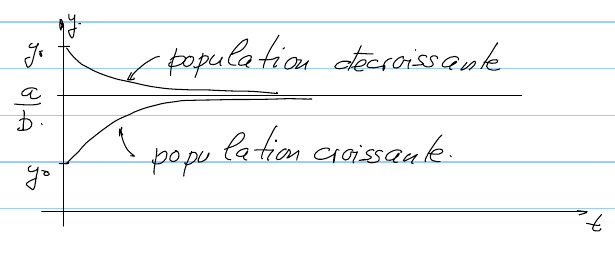
\includegraphics[scale=0.5]{images/verhulst}

\subsection{ED linéaires du premier ordre}
(revoir algèbre linéaire : Structure de la solution de Ax = b, A une matrice $n\times n$, b un vecteur $\in \R^n$)\\
Voir série 1, ex. 3, série 2, ex. 2

\subsubsection{Définitions}
Une Ed linéaire du premier ordre est de la forme 
\begin{boite}[0.5]
	\begin{equation}
		y' + p(x)\cdot y = q(x)
		\label{ed_lineraire}
		\end{equation}
\end{boite}
avec $p$ et $q$ des fonctions continues sur l'intervalle I.
\begin{boite}
	\evid{Définition :} Si dans $~\eqref{ed_lineraire}$ :
	\begin{enumerate}
		\item $q = 0$, l'équation est dite \underline{homogène}
		\item $q \neq 0$, l'équation est dite \underline{inhomogène} et $y' + p(x)\cdot y = 0$ est appelée l'équation homogène associée à $~\eqref{ed_lineraire}$
	\end{enumerate}
\end{boite}
On définit l'application $L\ :\ C^1(I) \to C^0(I)$ par\footnote{Ressemble à la dérivée mais fait un peu plus}
\begin{equation*}
	(L\eta)(x) = \eta'(x) + p(x)\eta(x)
\end{equation*}
et $~\eqref{ed_lineraire}$ devient 
\begin{boite}[0.25]
	\begin{equation*}
		Ly = q
	\end{equation*}
\end{boite}
$C^1(I)$ et $C^0(I)$ sont des espaces vectoriels (de dimension $\infty$), et l'application L est linéaire.
\begin{equation*}
	L(\alpha\eta_1 + \beta\eta_2) = \alpha L(\eta_1) + \beta L(\eta_2)
\end{equation*}
pour tout $\alpha,\beta \in \R \ , \ \eta_1,\eta_2 \in C^1(I)$\\
\evid{Démonstration :}\\
$(\alpha\eta_1 + \beta\eta_2)' + p(x)(\alpha\eta_1 + \beta\eta_2) = \alpha(\eta_1' + p(x)\eta_1) + \beta(\eta_2' + p(x)\eta_2)\qquad$ \#
Puisque l'équation est linéaire, nous pouvons appliquer nos connaissances en algèbre linéaire pour conclure que la solution générale de $~\eqref{ed_lineraire}$  est de la forme:
\begin{boite}[0.67]
	\begin{equation*}
		y(x) = y_p(x) + Cy_0(x) \qquad x\in I \ ,C\in\R
	\end{equation*}
\end{boite}
où $y_p(x)$ est une solution quelconque du problème inhomogène appelée solution particulière\footnote{d'où le $y_p$}, et $y_0$ une fonction non nulle dans le noyau  de $L \ , \ Ly_0 = 0$

\subsubsection{Méthode de résolution générale}
\begin{enumerate}[label=\roman*)]
	\item \underline{L'équation homogène peut être résolue par séparation des variables}\\
	$y' + p(x) = 0 \iff \ulcorner\frac{\deriv{y}}{y} = -p(x)\deriv{x} \to \ln(|y|) = -P(x)\lrcorner$, P une primitive de p. ($\ulcorner \lrcorner $ est la partie \enquote{recette})\\
		Donc (avec le choix +)
		\begin{boite}[0.47]
			\begin{equation*}
				y_0(x) = e^{-P(x)} \qquad ,x \in I
			\end{equation*}
		\end{boite}
	\item Recherche d'une solution particulière 
	 	\begin{enumerate}
	 		\item \evid{Méthode de la variation de la constante}\\
	 			on pose $y_p(x) = C(x)y_0(x) \qquad ,C(x)$ inconnu\\
	 			que l'on substitue dans l'équation inhomogène\\
	 			$\big(C(x)y_0(x)\big)' + p(x)\big(C(x)y_0(x)\big) = q(x)$\\
	 			$C'(x)y_0(x) + \underbrace{C(x)(y_0(x) + p(x)y_0(x))}_{=0}$\footnote{Correspond à un test : doit! être égal à 0}$ = q(x)$\\
	 			Donc on a que\\
	 			$C'(x) y_0(x) = q(x)$ où $C'(x) = \frac{1}{y_0(x)}q(x) = e^{P(x)}q(x)$\\
	 			donc $C(x) = \int\frac{1}{y_0(x)}q(x)\deriv{x} = \int e^{P(x)}q(x)\deriv{x}$\\
	 			et
	 			\begin{boite}[0.6]
	 				\begin{equation} 
	 					y_p(x) = \(\int e^{P(x)}q(x)\deriv{x}\)e^{-P(x)}
	 					\label{methode a)}
	 				\end{equation}
	 			\end{boite}
	 		\item \evid{La méthode du facteur intégrant}\\
	 		$y'(x) +p(x)y = q(x) \qquad |e^{P(x)} \qquad P(x)$ une primitive de p\\
	 		$\underbrace{y'e^P + \underbrace{pe^P}_{(e^P)'}y}_{=(e^Py)'} = qe^P$\\
	 		$\to e^{P(x)}y(x) = \int q(x) e^{P(x)} \deriv{x} \to ~\eqref{methode a)}$
	 		
	 		\item \evid{\enquote{méthode} des coefficients indéterminés} (si p(x) = constant)\\
	 			Cette méthode s'applique si $p(x)$ = constant et si $q(x)$ est une fonction polynôme, exponentielle, sin, cos, produits de polynômes avec des exponentielles, etc. On pose\\
	 			$\left.\begin{array}{ll}
	 				y_p(x) = C_1q(x) + C_2q'(x) & \text{\fbox{ si $Lq \neq 0$}}\\
	 				y_p(x) = C_1xq(x) + C_2xq'(x) & \text{\fbox{ si  $Lq = 0$}}
	 			\end{array}\right\}$
	 			avec $C_1, C_2$ à déterminer
	 	\end{enumerate}
\end{enumerate}

\subsubsection{exemples}
\begin{enumerate}
	\item $y' + x^2y = x^2 \qquad I=\R$
		\begin{enumerate} [label=\roman*)]
			\item Problème homogène $y'+x^2y = 0 \\
				\iff \frac{\deriv{y}}{y} = -x^2\deriv{x} \ , \ \ln(|y|) = -\frac{1}{3}x^3\\
				y_0(x) = e^{-\frac{1}{3}x^3} \qquad x\in\R$
			\item Solution particulière (variation de la constante) :\\
				$y_p(x) = C(x)e^{-\frac{1}{3}x^3}\qquad$ dans l'ED :\\
				$C'(x)e^{-\frac{1}{3}x^3} + \underbrace{C(x)e^{-\frac{1}{3}x^3}(-x^2)) + x^2C(x)e^{-\frac{1}{3}x^3}}_{=0 \text{ doit être 0 !!}} = x^2$\\
				Donc $C'(x) = x^2e^{\frac{1}{3}x^3} \to C(x) = e^{\frac{1}{3}x^3}$\\
				Ce qui nous fait que la solution particulière $y_p(x) = C(x)e^{-\frac{1}{3}x^3} = e^{\frac{1}{3}x^3}e^{-\frac{1}{3}x^3} = 1$
				\end{enumerate}
		\underline{La solution générale}\\
		 $y(x) = y_p(x) + Cy_0(x) = 1+Ce^{-\frac{1}{3}x^3} \qquad ,x\in\R, \forall C\in\R$
	\item $y' + 4y = \underbrace{3\sin(2x)}_{q(x)}  \qquad I=\R \quad p(x) = 4 =$ constante
		\begin{enumerate}[label=\roman*)]
			\item $y' + 4y = 0 \quad ,y_0(x) = e^{-4x} \ ,x\in \R$
			\item $p(x) = 4 =$ const et $Lq \neq 0$ \big(car $q(x) \neq Cy_0(x)$\big)\\
				Donc on va essayer : $y_p(x) = \underbrace{C_13}_{=C_1}\sin(2x) + \underbrace{C_26}_{=C_2}\sin(2x)$ (on rentre 3 et 6 dans les constantes)\\
				Mettre dans l'ED : $y_p'(x) + 4y_p(x) = 3\sin(2x)$\\
				$C_12\cos(2x) - 2C_2\sin(2x) + 4C_1\sin(2x) + 4C_2\cos(2x) = 3\sin(2x)$\\
				$\left.
					\begin{array}{ll}
						2C_1 + 4C_2 & = 0\\
						-2C_2 + 4C_1 & = 3
					\end{array}
				\right\} \to C_1 =  \frac{3}{5}, C_2 = -\frac{3}{10}$\\
				Donc $y_p(x) = \frac{3}{5}\sin(2x) - \frac{3}{10}\cos(2x)$
		\end{enumerate}
		\underline{Solution générale :}\\
		 $y(x) = y_p(x) + Cy_0(x) = \frac{3}{5}\sin(2x) - \frac{3}{10}\cos(2x) +  Ce^{-4x}$
	\item $(1+x^2)y' + xy = 4x\sqrt{1+x^2} \iff y' + \frac{x}{1+x^2}y = \frac{4x}{\sqrt{1+x^2}}$
		\begin{enumerate}[label=\roman*)]
			\item $y' + \frac{x}{1+x^2}y = 0\\
				\to \frac{\deriv{y}}{y} = -\frac{x}{1+x^2}\deriv{x}\\
				\to \ln(|y|) = -\frac{1}{2}\ln(1+x^2)\\
				\to y_0(x) = \frac{1}{\sqrt{1+x^2}}$
			\item $y_p(x) = C(x)y_0(x) = C(x)\frac{1}{\sqrt{1+x^2}}$ à mettre dans l'ED :\\
				$C'(x)\frac{1}{\sqrt{1+x^2}} + \underbrace{\ldots}_{=0} = \frac{4x}{\sqrt{1+x^2}}\\
				C'(x) = 4x \to  C(x) = 2x^2\\
				\to y_p(x) = C(x)y_0(x) = 2x^2\frac{1}{\sqrt{1+x^2}}$
		\end{enumerate}
		\underline{Solution générale :}\\
		$y(x) = y_p(x) + Cy_0(x) = \frac{2x^2}{\sqrt{1+x^2}} +C\frac{1}{\sqrt{1+x^2}} = \frac{2x^2+C} {\sqrt{1+x^2}}$
\end{enumerate}

\subsubsection*{Remarques concernant la méthode des coefficients indéterminés}
(voir série 2)
\begin{itemize}
	\item Si $q(x) = \somme{n}{i=1}{q_i(x)}$ (exemple : $y'-xy = 10\cos(x) + 2e^{3x}$, série 2, exercice 2 iii)
	on applique la méthode à chacun des $q_i$ et on somme les résultats.	
	\item si $q(x)$ fait intervenir des fonctions polynômes de degré d (exemple série 2, ex 2 iv) $y' + y = x^3$) alors il faut essayer une combinaison de $q, q',...,q^{(d)}$
	\item Si c'est trop compliqué, mieux vaut utiliser la méthode de la variation de la constante.
\end{itemize}

\subsubsection[Ricatti]{Équation de Ricatti (voir Séries 3.4)}
C'est une équation de la forme 
\begin{boite}
	\begin{equation}
		y' = a(x)y^2 + b(x)y + c(x)
		\label{ricatti}
	\end{equation}
\end{boite}
avec a,b,c des fonctions continues sur un intervalle I. C'est un exemple d'une équation que l'on ne sait pas résoudre en général, sauf si (pour une étrange et obscure raison) on connaît une solution, auquel cas on peut déterminer toutes les autres solutions. Donnée une solution $y_1(x)$, on pose
\begin{boite}[0.5]
	\begin{equation*}
		y(x) = y_1(x) + \frac{1}{u(x)}
	\end{equation*}
\end{boite}
avec $u(x)$ inconnu\\
que l'on substitue dans $~\eqref{ricatti}$ :\\
$y_1' - \frac{1}{u^2}u' = ay_1^2 + 2ay_1\frac{1}{u} + a \frac{1}{u} + by_1 + b\frac{1}{u} + c$
Les termes en $y_1$ (sauf $2ay_1\frac{1}{u}$) se compensent car $y_1$ est une solution.\\
Après multiplication par $u^2$ on obtient :\\
$u'+ 2ay_1u + a bu = 0 \iff $\fcolorbox{red}{white}{$u'+(2ay_1 + b)u = -a$} c'est une équation linéaire que l'on sait résoudre.\\
\evid{Remarque :} Si $c=0, y_1 = 0$ est une solution et on sait résoudre.\\
\evid{Remarque :} Si on pose $y(x) = -\frac{1}{a(x)}\frac{u'(x)}{u(x)}$ on trouve une équation linéaire du deuxième ordre.

\subsection{ED linéaires ordre 2, coeff. constants}
(série 3 consacrée à ce cas)

\subsubsection{Définitions}
Une ED linéaire du deuxième ordre à coefficients constants est de la forme
\begin{boite}[0.5]
	\begin{equation}
		ay''+by'+cy = q(x)
		\label{second ordre lineaire}
	\end{equation}
\end{boite}
où $a\in \R^*\ , \ b,c \in\R$ et $q$ une fonction continue sur un intervalle I.\\
Cette équation est de la forme $Ly = q$ avec 
\begin{equation*}
(L\eta)(x) = a\eta''(x) + b\eta'(x) + \eta(x)
\end{equation*}
et L est une application linéaire de $C^2(I) \to C^0(I)$
\newpage
\subsubsection{Méthode de résolution}
Le procédé de résolution est similaire au cas du premier ordre.
\begin{enumerate}[label=\roman*)]
	\item \fcolorbox{red}{white}{\underline{Méthode de résolution de l'équation homogène}}\footnote{$Ly=0$}\\
	La solution est de la forme 
	\begin{boite}
		\begin{equation*}
			y_h(x) = C_1y_1(x) + C_2y_2(x)\ \qquad C_1,C_2 \in\R
		\end{equation*}
	\end{boite}
	On essaye $y(x) = e^{\lambda x}$\footnote{ça marche car l'équation est à coefficients constants}. On substitue dans $ay'' + by' + cy = 0$ et on trouve
	\begin{equation*}
		e^{\lambda x}\underbrace{(a\lambda^2 + b\lambda + c)}_{=0\text{ encore un test}} = 0
	\end{equation*}
	1er cas: $ b^2-4ac > 0 \to $ deux solutions réelles pour $\lambda : \ \lambda_1,\lambda_2$\\
	La solution générale de l'équation homogène est :
	\begin{boite}
		\begin{equation*}
			y_n(x) = C_1\underbrace{e^{\lambda_1 x}}_{=y_1(x)} + C_2 \underbrace{e^{\lambda_2 x}}_{=y_2(x)} \qquad ,x\in\R \ (x\in I), C_1,C_2 \in \R
		\end{equation*}
	\end{boite}
	2\ts{ème} cas : $b^2 - 4ac = 0$ seulement une solution réelle $\lambda \in\R$.\\
	La solution générale de l'équation homogène est :
	\begin{boite}
		\begin{equation*}
			y_n(x) = C_1\underbrace{e^{\lambda x}}_{=y_1(x)} + C_2\underbrace{xe^{\lambda x}}_{=y_2(x)}
		\end{equation*}
	\end{boite}
	3\ts{ème} cas : $b^2-4ac < 0$ : deux solutions complexes conjuguées\\
	($\lambda = \alpha+ i\beta \ , \ \overline{\lambda} = \alpha - i\beta \ ,\alpha,\beta \in \R)$\\
	La solution générale réelle de l'équation homogène est :
	\begin{boite}
		\begin{equation*}
			y_n(x) = Ce^{\lambda x} + \overline{C}\underbrace{\overline{e^{\lambda x}}}_{=e^{\overline{\lambda}x}} \qquad \in \R, \ \forall C \in \C
		\end{equation*}
	\end{boite}
	mais $e^{\lambda x} = e^{(\alpha + i\beta) x} = e^{\alpha x}e^{i\beta x} = e^{\alpha x}(\cos(\beta x) + i\sin(\beta x))$\\
	$C = \frac{1}{2}(C_1+iC_2) \quad ,C_1 = 2\Re(C), C_2 = 2\Im(C)$
	\begin{boite}
		\begin{equation*}
			y_n(x) = C_1\underbrace{e^{\alpha x}\cos(\beta x)}_{=y_1(x)} + C_2 \underbrace{e^{\alpha x}\sin(\beta x)}_{=y_2(x)}
		\end{equation*}
	\end{boite}
	\item \fcolorbox{red}{white}{\underline{Recherche d'une solution particulière de l'équation complète}}\\
	Soient $y_1(x)$ et $y_2(x)$ les deux solutions du problème homogène construites sous i). :\\
	\evid{Méthode de la variation des constantes}\\
	On pose\footnote{boites rondes : C dérivés, boîtes carrées : C pas dérivés} $y(x) =\text{\fbox{$C_1(x)y_1(x) +C_2(x) y_2(x)$}}_{(0)}$\\
	$y'(x) = \text{\ovalbox{$C_1'(x)y_1(x) +C_2'(x)y_2(x)$}}_{(1)} + \text{\fbox{$C_1y_1'(x) + C_2(x)y_2'(x)$}}_{(1)}$ \\
	$y''(x) = \text{\ovalbox{$C_1'(x)y_1'(x) + C_2'(x)y_2'(x)$}}_{(2)} + \text{\fbox{$C_1(x)y_1''(x) + C_2(x)y_2''(x)$}}_{(2)}$\\
	On obtient
	\begin{equation*}
		\underbrace{a\cdot\fbox{(2)} + b\cdot\fbox{(1)} + c\cdot\fbox{(0)}} + \ovalbox{(2)} = q
	\end{equation*}
	$C_1(x)\underbrace{\big(ay_1''+by_1'+y_1\big)}_{=0\text{ car $y_1$ une solution de} Ly_1 = 0} + C_2(x)\underbrace{\big(ay_2'' + by_2' + cy_2\big)}_{=0\text{ car $y_2$ une solution de} Ly_2= 0} = 0$
	 trouve donc
	\begin{boite}
		\begin{equation*}
			C_1'(x)y_1(x) + C_2'(x)y_2(x) = 0 \qquad \text{choix délibéré}
		\end{equation*}
		\begin{equation}
		C_1'(x)y_1(x) + C_2'(x)y_2(x) = \frac{1}{a}q(x)
		\label{solution methode variation des constantes}
		\end{equation}
	\end{boite}		
	ou encore :
		\begin{boite}
		$\begin{pmatrix}
		y_1(x) & y_2(x)\\
		y_1'(x) & y_2'(x)
		\end{pmatrix}
		\cdot 
		\begin{pmatrix}
		C_1'(x)\\
		C_2'(x)
		\end{pmatrix}
		=
		\begin{pmatrix}
		0\\
		\frac{1}{a}q(x)
		\end{pmatrix}$ (apprendre par coeur)	
		\end{boite}
		et on trouve (voire la remarque en bas)\\
		$\begin{pmatrix}
		C_1'(x)\\
		C_2'(x)
		\end{pmatrix}
		=
		\begin{pmatrix}
		y_1(x) & y_2(x)\\
		y_1'(x) & y_2'(x)
		\end{pmatrix}^{-1}
		\cdot
		\begin{pmatrix}
		0\\
		\frac{1}{a}q(x)
		\end{pmatrix}$\\
		puis on intègre pour obtenir $C_1(x)$ et $C_2(x)$ et on a la solution particulière.\\
		%%%%%%%%%%%%%%%%%%%%%%%%%%%%%%%%%
		%%%%%%Depuis la c'est moche%%%%%%
		%%%%%%%%%%mais ça passe%%%%%%%%%
		%%%%%%%%on commente%%%%%%%%%%%%
		%%%%%%%% parce que ça passe plus%%%%%%%%%%%%%%
		%%%%%%%%%%%%%%%%%%%%%%%%%%%%%%%%%
%		\begin{frame}[ %%%[obligatoire ?? pourquoi ?%%%
%		\tikz[baseline=(A.base),remember picture] \node(A) {$y_p(x)$}; $= C_1(x)y_1(x) + C_2(x)y_2(x)$		
		\item %%%mettre ce truc plus à gauche%%%
		\begin{boite}
			 La solution générale de l'équation est :	\\
				$\qquad y(x)$\tikz[baseline=(B.base),remember picture] \node(B) {$= y_p(x)$};$  + y_h(x) = y_p(x) + C_1y_1(x) + C_2y_2(x)$\\
		avec $x\in I$ (domaine de q) et $C_1,C_2 \in \R$
		\end{boite}
%		\begin{tikzpicture}[remember picture, overlay]
%		 \draw[->,ultra thick,green,opacity=.5] (A) to (B);
%		\end{tikzpicture}
%	\end{frame}
	%%%%%%%%%%%%%%%%%%%%%%%%%%%%%%%%%%%%
	%%%%%%%%%%%%fin de moche%%%%%%%%%%%%
	%%%%%%%%%%%%%%%%%%%%%%%%%%%%%%%%%%%%
	\begin{boite}
	Remarque : La fonction \\
	$w(x):= \det
	\begin{pmatrix}
	y_1(x) & y_2(x)\\
	y_1'(x) & y_2'(x)
	\end{pmatrix}
	 = y_1(x)y_2'(x) - y_1'(x)y_2(x)$\\
	 est appelée le Wronskien des solutions de $y_1$ et $y_2$. Il est non nul ($\forall x$) si les solutions $y_1$ et $y_2$ ne sont pas un multiple l'une de l'autre, c'est à dire si $y_1$ et $y_2$ sont linéairement indépendants
	 \end{boite}

	 \evid{méthode des coefficients indéterminés pour ii)}\\
	 On pose\\
	 $\left\{
	 	\begin{array}{ll}
	 		y_p(x) = & \text{ Combinaison linéaire des dérivées de }q : q', q'',\ldots\\
	 			& \text{si } Lq\neq 0 \text{ (q n'est pas une solution de l'équation homogène)}
	 	\end{array}
	 \).\\
	 \left\{
	 	\begin{array}{ll}
	 		y_p(x) = xq & \text{plus les dérivées }(xq)', (xq)'',\ldots\\
	 			& \text{si }Lq = 0,\ L(xq) \neq 0
	 	\end{array}
	\).\\
	\left\{
		\begin{array}{ll}
			y_p(x) = x^2q & \text{plus les dérivées }(x^2q)', (x^2q)'',\ldots\\
	 			& \text{si }Lq = 0,\ L(xq) = 0
		\end{array}
	\).
	$	 
	 
	 Mêmes remarques que dans le cas des équations linéaires du premier ordre
\end{enumerate}
   
\subsubsection{Exemples}
\begin{enumerate}[label=\arabic*)]
	 	\item $y'' + 4y = e^x \qquad \big(=q(x)\big) \qquad x\in\R$
	 		\begin{enumerate}[label=\roman*)]
	 			\item 
	 				$\lambda^2 + 4 = 0 \ , 
	 				\left\{
	 					\begin{array}{ll}
	 						\lambda_1 & = 2i \quad , \quad \lambda_2 = \overline{\lambda_1} = -2i\\
	 						 & = \alpha + i\beta, \quad \alpha =0,\ \beta =2\\
						\end{array}
					\).$\\
					$y_1(x) = \cos(2x) \qquad y_2(x) = \sin(2x)\\
				 	y_n(x) = C_1y_1(x) + C_2y_2(x) = C_1\cos(2x) + C_2\sin(2x)$
	 			\item Méthode des coefficients indéterminés.\\
	 				$Lq \neq 0$ car $e^x \neq C_1\cos(2x) + C_2\sin(2x)$\\
	 				Donc on essaye $y_p(x) = Ae^x$ (+dérivées, mais c'est encore $e^x$).\\
	 				$Ae^x + 4Ae^x = e^x \to A=\frac{1}{5}$.\\
	 				Donc $y_p(x) = \frac{1}{5}e^x$
	 			\item La solution générale est :\\
	 			$y(x) = y_p(x) + y_h(x) = \frac{1}{5}e^x + C_1\cos(2x) + C_2\sin(2x) \\
	 			 x\in \R \ , \ C_1,C_2\in\R$
		 	\end{enumerate}
		 \item  $y'' + y = \tan(x) \qquad x\in I (]-\frac{\pi}{2}, \frac{\pi}{2}[)$
		  \begin{figure}
		 \centering
		 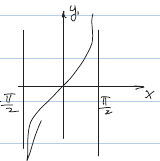
\includegraphics[scale=1]{images/tanx}
		 \caption{La fonction $\tan(x)$, contenue dans l'intervalle $I = ]-\frac{\pi}{2},\frac{\pi}{2}[$}
		 \end{figure}
		 	\begin{enumerate}
		 		\item $\lambda^2 + 1 = 0 \ , \ \lambda_1 = i, \lambda_2 = -i = \overline{\lambda}$\\
		 			$y_n(x) = C_1\underbrace{\cos(x)}_{=y_1(x)} + C_2\underbrace{\sin(x)}_{=y_2(x)}$
		 		\item Variation des constantes\\
		 			$\begin{pmatrix}
			 		\cos(x) & \sin(x)\\
			 		-\sin(x) & \cos(x)
			 		\end{pmatrix}
			 		\cdot
			 		\begin{pmatrix}
			 		C_1'(x)\\
			 		C_2'(x)
			 		\end{pmatrix}
			 		=
			 		\begin{pmatrix}
			 		0\\
			 		\tan(x)
			 		\end{pmatrix}$\\
			 		$\begin{pmatrix}
			 		C_1'(x)\\
			 		C_2'(x)
			 		\end{pmatrix}
			 		=
			 		\begin{pmatrix}
			 		\cos(x) & -\sin(x)\\
			 		\sin(x) & \cos(x)
			 		\end{pmatrix}
			 		\cdot
			 		\begin{pmatrix}
			 		0\\
			 		\tan(x)
			 		\end{pmatrix}
			 		=
			 		\begin{pmatrix}
			 		\frac{-\sin^2(x)}{\cos(x)}\\
			 		\sin(x)
			 		\end{pmatrix}$\\
			 		Donc\\
			 		$C_1'(x) = \cos(x) - \frac{1}{\cos(x)}$\\
			 		$C_2'(x) = \sin(x)$\\
			 		On trouve (voir série 4 pour une primitive de $\frac{1}{\cos(x)}$)\\
			 		$C_1(x) = \sin(x) - \ln\(\left|\frac{1+\sin(x)}{\cos(x)}\)|\)$\\
			 		$C_2(x) = -\cos(x)$\\
			 		Donc $y_p(x) = C_1(x)\cos(x) + C_2(x)\sin(x) = -\cos(x)\ln\(\left|\frac{1+\sin(x)}{\cos(x)}\)|\)$ (discuter cette fonction + voir série 4, répétition Analyse I)
		 		\item solution générale : $y(x) = y_p(x) + C_1\cos(x) + C_2\sin(x) \,x\in I \ , C_1,C_+ \in \R$
		 	\end{enumerate}
\end{enumerate}
	 
\subsection{ED linéaires ordre 2, coeff. variables}
\subsubsection{Équations homogènes}
C'est une équation de la forme
\begin{boite}
	 \begin{equation}
	 	y'' + p(x)y' + q(x)y = 0
		\label{equation coeff variable homogene}
	\end{equation}
\end{boite}
avec $p,q$ des fonctions sur un intervalle I.\\
\underline{Il n'existe pas de méthode de résolution générale !}\\
\begin{boite}
\evid{Réduction de l'ordre :}\\
Si on connait une solution non nulle y, de ~\eqref{equation coeff variable homogene} on pose\\
\fcolorbox{red}{white}{$y(x) = U(x) \cdot y_1(x)$}\\
avec U une prmitive d'une nouvele fonction inconnue u
\end{boite}
On obtient \\
$U''y_1 + 2U'y_1' + U/y_1'' + p(x)U'y_1' + p(x) U/y_1' + q(x)U/y_1(x) = 0$\\
les / s'annulent car $y_1$ est une solution\\
Donc on a, en utilisant que par définition $U' = u$
\begin{equation*}
	y_1(x)u' + (2y_1'(x) + p(x)y_1)u = 0
\end{equation*}
Ce qui est une équation linéaire homogène du premier ordre que l'on peut résoudre par séparation des variables pour trouver u; puis on détermine une primitive U de u pour trouver une deuxième solution $y_2 = Uy$, linéairement indépendante de $y_1$

\subsubsection{Équation inhomogène}
C'est une équation de la forme 
\begin{equation}
	y'' + p(x)y' + q(x)y = f(x)
	\label{second_ordre_coeff_variable_inhomogene}
\end{equation}
avec $p$,$q$ et $f$ continues sur un intervalle I.
\begin{enumerate}[label=\roman*)]
	\item \underline{La méthode de éa variation des constantes} marche exactement comme dans le cas à coefficients constants (Voir le chapitre 0.4.2). Soient $y_1$ et $y_2$ deux solutions linéairement indépendantes du problème homogène associé ~\eqref{second_ordre_coeff_variable_inhomogene}. Alors on pose
	\begin{equation*}
		y_h(x) = C_1(x)y_1(x) + C_2(x)y_2(x)
	\end{equation*}
	et on trouve
	\begin{boite}[0.4]
	$\begin{pmatrix}
		C_1'\\
		C_2'
	\end{pmatrix}
	=
	\begin{pmatrix}
		y_1 & y_2\\
		y_1' & y_2'
	\end{pmatrix}^{-1}
	\begin{pmatrix}
	0\\
	f
	\end{pmatrix}$
	\end{boite}
	(voir le chapitre 0.4.2 pour les détails
	\item \underline{Transformation à une équation à coefficients constants par changement de variable}\\
	voir série 4 pour un exemple
\end{enumerate}

\subsection{ED linéaires ordre $> 2$,  coeff. constants, }
Soit l'ED:
\begin{boite}[0.75]
	\begin{equation*}
		a_{n}y^{(n)}+a_{n-1}y^{(n-1)} + \ldots + a_1y' + y_0y = q(x)
	\end{equation*}
\end{boite}
$a_0,\ldots,a_n \in \R \quad a_0 \neq 0$, $q(x)$ une fonction continue sur un intervalle I.
\begin{enumerate}[label=\roman*)]
	\item \underline{Résolution de l'équation homogène}\\
		on essaye $y(x) = e^{\lambda x}$ et on trouve
		\begin{equation*}
		a_m\lambda^n + a_{n-1}\lambda^{n-1} + \ldots + a_0 = 0
		\end{equation*}
		\begin{equation*}
			= a_n(\lambda - \lambda_1)^{p_1} \ldots (\lambda-\lambda_m)^{p_m}
		\end{equation*}
		avec $1\leq m \leq n \quad , \quad 1\leq p_i \quad i=1,\ldots,m$ et $p_1+\ldots+p_m = n$\\
		La solution générale du problème homogène  est\\
		$y_h(x) = \underbrace{P_1(x)}_{\mathclap{\substack{\text{Polynôme général de}\\ \text{ degré }  p_1-1}}}e^{\lambda_1x} + \ldots + P_m(x)e^{\lambda_mx}$ % a améliorer
		Cas particulier : $\lambda_i \neq \lambda_j$ pour tout $i,j$. Dans ce cas, $p_1=1 \ i = 1\ldots n$ et la solution du problème est \\
		$y_h(x) = C_1e^{\lambda_1x} + \ldots + C_ne^{\lambda_mx}$\\
		$C_i\in \R \ , \ i = 1,\ldots,n$
	\item  
		\begin{itemize}
			\item la méthode de la variation des constantes se généralise
			\item la méthode des coefficients indéterminés se généralise (voir série 4)
		\end{itemize}		 
	\item solution générale \fcolorbox{red}{white}{$y(x) = y_p(x) + y_n(x)$}
	voir le chapitre 7 pour une autre méthode de résolution
\end{enumerate}
\evid{Exemples}\\
$y''-y = 2x^3 = q(x) \qquad I = \R$
\begin{enumerate}
	\item 	$\lambda^3-1 = 0$
			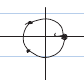
\includegraphics[scale=0.5]{images/cercle_trigo}
			$\qquad 
			\left\{\begin{array}{l}
				\lambda_1= 1\\
				\lambda_2 =-\frac{1}{2} + i \frac{\sqrt{3}}{2} = \alpha + i\beta\\
				\lambda_3 = \overline{\lambda_2}
			\end{array}\right.\\ $
			$y_h(x) = C_1e^x + C_2e^{-\frac{1}{2}x}\coss{\frac{\sqrt{3}}{2}x} + C_3e^{-\frac{1}{2}x}\sin\(\frac{\sqrt{3}}{2}x\))$ (comme discuté pour les équations du deuxième ordre)\\
		
	\item $q(x)$ n'est pas solution du problème homogène (car $q''-q \neq 0$). On essaye donc une combinaison linéaire de $q$ et de ses dérivées.\\
		$\begin{array}{l}
		y_p(x) = Ax^3 + Bx^2 + Cx + D\\
		y_p'''(x) = 6A
		\end{array}$\\
		Substituer dans $y'''-y = 2x^3$
		\begin{align*}
			x^3: & -A = 2 & A=-2\\
			x^2: & -B = 0 & B=0 \\
			x: & -C=0 & C=0\\
			1: & 6A-D = 0 & D = 6A = -12
		\end{align*}
		Donc $y_p(x) = -2x^3-12$ (vérifier !)
	\item Solution générale : $y(x) = y_p(x) + \underbrace{y_h(x)}_{\mathclap{\forall C_1,C_2,C_3 \in \R}} \qquad x\in \R$
\end{enumerate}
\subsection{Solutions qualitatives, méthodes des isoclines} (voir aussi le chapitre 7)\\
ED du premier ordre. On suppose que l'on puise écrire l'ED sous la forme 
\begin{boite}[0.17]
$y' = f(x,y)$
\end{boite}
\underline{Interprétation géométriques} en chaque point ($x_0,y_0$) on connaît la pente d'une solution $y(x)$ qui satisfait $y_0(x) = y_0$, car $y'(x_0) = f\big(x_0,y(x_0)\big) = f(x_0,y_0)$
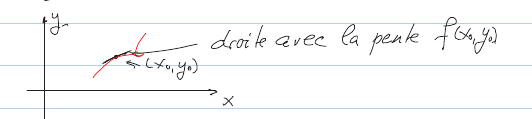
\includegraphics[scale=0.5]{images/isocline1}\\
\underline{méthode des isoclines} : on considère l'ensemble des points (x,y) tels que $f(x,y) = c$, pour $c$ donné. Nous verrons que ceci donne pour chaque C (pour un f générique) un ensemble de courbes\\
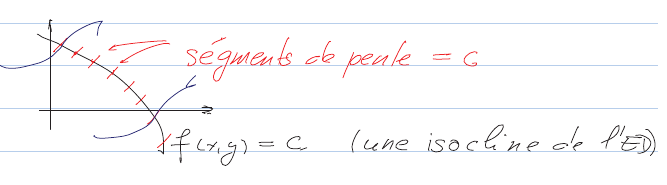
\includegraphics[scale=0.5]{images/isocline2}\\
\evid{Exemple :}\\
ED: $y' = x^2+y^2 = f(x,y)$
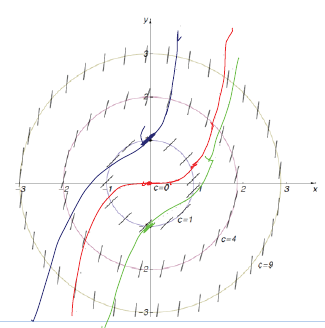
\includegraphics[scale=0.4]{images/isocline3}

\subsection{Théorème d'existence et d'unicité}
\begin{boite}
	Théorème : Soit l'ED $y'=f(x,y)$ avec $f : D\to \R$
	\begin{center}
		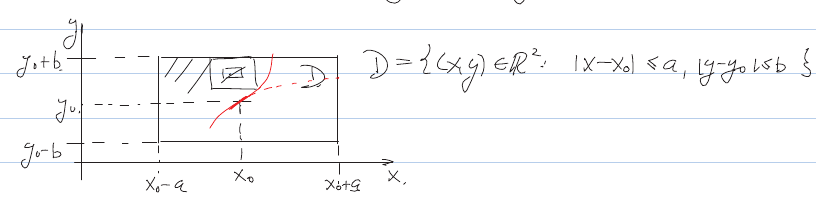
\includegraphics[scale=0.65]{images/theo_existence}
	\end{center}
	$\left.
		\begin{array}{l}
			f \text{ continue sur } D\\
			\frac{\delta f}{\delta y} \text{ continue sur } D
		\end{array}		
	\)\}$ 
	alors il existe exactement une solution de l'ED dans un voisinage de $x_0$ telle que $y(x_0) = y_0$
\end{boite}
\evid{Remarque} Puisque D est fermé, la condition que $f$ et $\frac{\delta f}{\delta y}$ soient continues implique que $f$ et $\frac{\delta f}{\delta y}$ soient bornée sur D\\
\evid{Remarque :} Le théorème s'applique à ($x_0',y_0') \in D$ arbitraire pour un rectangle $D' \subset D$ centré à $(x_0',y_0')$\\
\evid{Contre exemple :} (une condition sur $\frac{\delta f}{\delta y}$ est indispensable).\\
$y' = 3|y|^{\frac{2}{3}} = f(x,y)\\
y(x) = 0 \quad , \quad x\in \R$ est une solution.\\
$y(x) = (x-C)^3 \quad , \quad x\in\R$ est une solution, pour tout $\C\in\R$\\
Donc la solution qui satisfait $y(0) = 0$ n'est pas unique.\\
une infinité de solutions telles que $y(0) = 0$ par \enquote{chirurgie}.\\
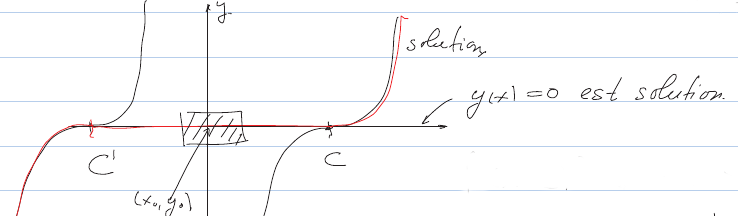
\includegraphics[scale=0.5]{images/sol_chirurgie}\\
\textcolor{red}{Solution par chirurgie : $y(x) = 
	\left\{
		\begin{array}{lll}
			(x-C)^3 & \pour & x>C\\
			0 & \pour & C' \leq x\leq C\\
			(x-C')^3 & \pour & x<C'
		\end{array}
	\).$}\\
\evid{Explication :}\\
$f(x,y) = 3|y|^{\frac{2}{3}} = 
\left\{
	\begin{array}{ll}
		3y^{\frac{2}{3}} & y\geq 0\\
		3(-y)^{\frac{2}{3}} & y<0
	\end{array}
\).$\\
et donc pour $\frac{\delta f}{\delta y} (x,y) = 
\left\{
	\begin{array}{ll}
	2y^{-\frac{1}{3}} & y>0\\
	-2y^{-\frac{1}{3}} & y<0
	\end{array}
\).$\\
Le théorème ne s'applique donc pas à un rectangle qui contient des points où $y=0$

\section[Espace \rn, rappels]{L'espace $\R^n$, rappels, définitions, notations}
(trait d'union philosophique : \href{http://fr.wikipedia.org/wiki/L%27Insoutenable_L%C3%A9g%C3%A8ret%C3%A9_de_l%27%C3%AAtre}{L'insoutenable légèreté de l'être)}
\begin{multicols}{2}
\evid{Analyse I :}
\begin{itemize}
	\item Produit cartésien
	\item ensembles ouverts, fermés, etc-
	\item Suites numériques, sous-suites, BW
	\item Suite de Cauchy
	\item Définition de limite
	\item Définition de continuité
\end{itemize}
\evid{Algèbre linéaire:}
\begin{itemize}
	\item espace vectoriel
	\item Produit scalaire
	\item définition d'une norme
\end{itemize}
\end{multicols}
$\R^n = \R\times \R\times\ldots\times\R \qquad $\enquote{$\times$}$ =$ produit cartésien\\
$\textbf{x}\in\R,\ \textbf{x}=(x_1,...,x_n)$ un point de $\R^n$\\
pour n = 2, \textbf{x} = $(x,y), n=3, x=(x,y,z)$ (autres notations possibles)
\subsection{$\R^n$ un espace vectoriel} (voir algèbre linéaire)
\textbf{x} = 
$\begin{pmatrix}
x_1\\
\ldots\\
x_n
\end{pmatrix}
\textbf{x}$ un vecteur (ou matrice $n\times 1$)\\
$\left< \textbf{x},\textbf{y}\)> = \somme{n}{i=1}{x_iy_i}$ produit scalaire "canonique"\\
$\left<\textbf{x},\textbf{y}\)> = \textbf{x}^T\cdot \textbf{y}^T$ produit des matrices
\subsection{$\R^n$ est un espace vectoriel normé}
La fonction $||\underbracket{\ldots}|| : \R^n \to \R$\\
$||\textbf{x}|| = \sqrt{\left<\textbf{x},\textbf{x}\)>} = \sqrt{\somme{n}{i=1}{x_i^2}}$\\
est une norme sur $\R^n$ (=largeur du vecteur \textbf{x})\\
Pour $n=1$ c'est simplement la fonction valeur absolue
\begin{boite}
\evid{Propriétés :}
\begin{enumerate}[label=\roman*)]
	\item $||\textbf{x}|| \geq 0 \quad , \quad \forall x\in\R^n \quad, \quad ||\textbf{x}|| = 0 \iff \textbf{x} = 0$
	\item $||\lambda\textbf{x}|| = \lambda||\textbf{x}|| \forall\textbf{x} \in \R^n, \lambda \geq 0$
	\item inégalité triangulaire $||\textbf{x}+\textbf{y}|| \leq ||\textbf{x}|| + ||\textbf{y}||$
\end{enumerate}
\end{boite}
\evid{Inégalité de Cauchy-Schwarz}\\
$\left< x,y \)> \leq ||x|| \cdot ||y||$\\
Car \fcolorbox{red}{white}{$\left< \textbf{x},\textbf{y}\)> = ||\textbf{x}||\cdot||\textbf{y}||\cos(\theta)$}
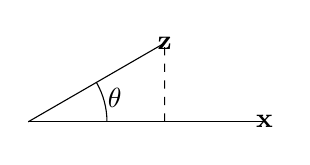
\begin{tikzpicture}
	\draw (0,0) -- (3,0) node{\textbf{x}};
	\draw (0,0) -- (30:2) node{\textbf{z}};
	\draw (1,0) arc (0:30:1);
	\draw (1.1,0.3) node{$\theta$};
	\draw [dashed] (1.732,0) -- (30:2); 
\end{tikzpicture}\\
\evid{Distance entre deux points de $\R^n$}\\
$d(\textbf{x},\textbf{y}) := ||\textbf{x}-\textbf{y}||$
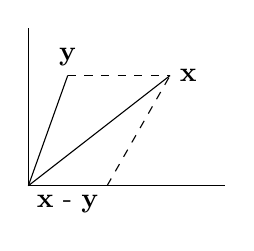
\begin{tikzpicture}
	\draw (0,0) -- (2.5,0);
	\draw (0,0) -- (0,2);
	\draw (0,0) -> (1,0)node[midway, below]{\textbf{x} - \textbf{y}};
	\draw (0,0) -> (1.8, 1.4) node[right]{\textbf{x}};
	\draw [dashed] (1,0) -- (1.8,1.4);
	\draw (0,0) -- (0.5,1.4) node[above]{\textbf{y}};
	\draw [dashed] (0.5,1.4) -- (1.8,1.4) ; 
\end{tikzpicture}\\
\evid{Propriétés}
\begin{enumerate}
	\item $d(\textbf{x},\textbf{y}) \geq 0$ et $d(\textbf{x},\textbf{y}) =0 \iff \textbf{x} = \textbf{y}$
	\item $d(\textbf{x},\textbf{y}) = d(\textbf{y},\textbf{x})$
	\item inégalité triangulaire : $d(\textbf{x},\textbf{y}) \leq d(\textbf{x},\textbf{z}) + d(\textbf{z},\textbf{y} \forall \textbf{x}, \textbf{y}, \textbf{z}$
\end{enumerate}

\subsection{Sous-ensembles de $\rn$}
\begin{boite}
	\evid{Définition :} Soit $\textbf{a}\in\rn $ et $r>0$. L'ensemble
	\begin{equation*}
		B(\textbf{a}, r) = \{\textbf{x}\in\rn : d(\textbf{x},\textbf{a}) < r\}
	\end{equation*}
	est appelé \enquote{boule ouverte de centre \textbf{a} et rayon r}
\end{boite}	
	n=2 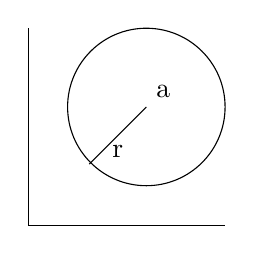
\begin{tikzpicture}[scale = 0.5]
		\draw (0,0) -- (5,0);
		\draw (0,0) -- (0,5);
		\draw (3,3) circle(2) node[above right]{a};
		\draw (3,3) -- (1.55,1.55) node[midway,below]{r};
	\end{tikzpicture}
\begin{boite}
	\evid{Définition :} Un sous-ensemble $X\subset \rn$ est dit ouvert si pour tout $\textbf{x} \in X$, il existe $r>0$, tel que $B(\textbf{x},r)\subset X$ %{dessin ensemble x, loupe}
	\end{boite}
\begin{boite}
	\evid{Définition} Un sous-ensemble $X\subset \rn$ est fermé si \R$\setminus X$ est ouvert
\end{boite}
Pour le bord d'un ensemble, l'intérieur, etc. on a aussi les mêmes définitions que pour \R avec $]a-r,a+r[$ remplacées par $B(\textbf{a},r)$\\
\evid{Exemple :} $X = B(0,1) \subset \R^2$

\subsection{Suites dans $\rn$}
\begin{boite}
	\evid{Définition :} On appelle suite des points de \rn toute application $f:\N\to \rn$
\end{boite}
\evid{Notation} On pose $\textbf{x}_n = f(n)$ et on écrit ($\textbf{x}_n)_{n\geq 0}$ ou encore $x_0,\ldots$ pour la suite.\\
\begin{boite}
	\evid{Définition : }une suite ($\textbf{x}_k$) dans \rn est convergente et admet pour limite (ou converge vers) \textbf{a}$\in \rn$ ; et l'on écrit
	\begin{equation*}
		\limite{\ninf}{\textbf{x}_n} = \textbf{a}
	\end{equation*}
	Si pour tout $\epsilon>0$ il existe $n_0 \in \N$, tel que pour tout $n\geq n_0$ on aie $\textbf{x}_n \in B(\textbf{a},\epsilon)$ (c'est à dire $d(\textbf{x}_n,\textbf{a}) = ||\textbf{x}_n - \textbf{a}|| < \epsilon$)
\end{boite}
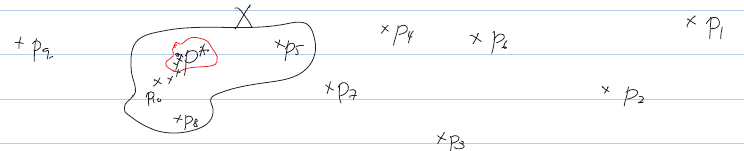
\includegraphics[scale=0.5]{images/converge}\\
\underline{Autres notations identiques} : (voir analyse I)
\begin{itemize}
	\item Définition d'une suite de Cauchy
	\item Sous-suites, Théorème de B.W.
	\item le fait que \rn est complet := "toute suite de Cauchy" d'éléments de \rn converge vers un élément de \rn" ($\Q^n$ n'est pas complet). \rn est un espace vectoriel normé.
	\end{itemize}

	\begin{enumerate}
\item ~
\begin{boite}
 \underline{Définition }(limite épointée)\\
La fonction $f:\rtor$ admet pour limite (épointée) $l \in \R$ lorsque x tend vers $x^*$. Si pour toute suite $(x_k)_{k\geq 0}, x_k \in \mathbf{D}(f) \setminus \{x^*\}$ tel que $\limite{\ninf} x_k = x^{*}$. La suite $(y_k), y_k = f(x_k)$ converge et $\limite{k\to\infty} y_k = l (\iff$ la même limite pour toutes les suites admises) 
\end{boite}

	\item~
\begin{boite}
				\underline{Définition }(limite du doc de référence)\\
	La fonction $f:\rtor$ admet pour limite $l \in \R$ lorsque x tend vers $x^*$. Si pour toute suite $(x_k)_{k\geq 0}, x_k \in \mathbf{D}(f)$ tel que $\limite{k\to\infty} x_k = x^{*}$. La suite $(y_k), y_k = f(x_k)$ converge et $\limite{\ninf} y_k = l (\iff$ la même limite pour toutes les suites admises) 
\end{boite}
\begin{boite}
\evid{Notations :}

	\begin{enumerate}
		\item $\limite{\ninf} f(x) \equiv \underset{x \neq x^*}{\lim\limits_{x \to x^*}} f(x) = l$ Limite épointée
		\item $\limite{\ninf} f(x) = l$ Limite selon le document de référence.
	\end{enumerate}
\end{boite}
\end{enumerate}
\begin{boite}
	\evid{Définition} (continuité): Une fonction $f: \rn \to \Rm$ est continue en $\textbf{x}_0 \in D(f)$, si
	\begin{equation*}
		\llimite{\textcolor{red}{\circled{1}} + \circled{2} \textbf{x} \to \textbf{x}_0}{\textcolor{red}{\circled{1} \textbf{x} \neq \textbf{x}_0}}{f(\textbf{x})} = f(\textbf{x}_0)
	\end{equation*}
	avec \textcolor{red}{\circled{1} existence de la limite et égalité} et \circled{2} existence suffit
\end{boite}
\subsection{Autres normes sur \rn}
	\begin{multicols}{3}
	\begin{center}	
		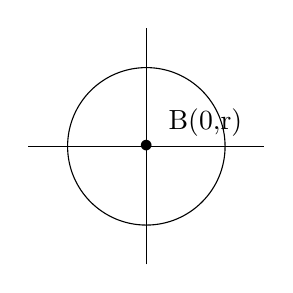
\begin{tikzpicture}
			\draw (0,0) circle(1) node{$\bullet$};
			\draw (-1.5,0) -- (1.5,0) node[near end, above]{B(0,r)};
			\draw (0,-1.5) -- (0,1.5);
		\end{tikzpicture}\\
		\fcolorbox{red}{white}{$||\textbf{x}|| = \sqrt{\somme{n}{i=1}{x_i^2}}$}\\
		~\\
		$||\ \ ||_2$\\
		\columnbreak
		\begin{tikzpicture}
			\draw (-1,1) -- (1,1) node[near end, above]{r};
			\draw (-1,-1) -- (1,-1);
			\draw (1,1) -- (1,-1) node[near end, right]{r};
			\draw (-1,1) -- (-1,-1);
			\draw (0,1.5) -- (0,-1.5);
			\draw (-1.5,0) -- (1.5,0);
		\end{tikzpicture}\\
		\fbox{$||\textbf{x}|| = \underset{i=1,...,n}{\max}\{|x_1|...|x_n|\}$}\\
		~\\
		$||\ \ ||_\infty$\\
		\columnbreak
		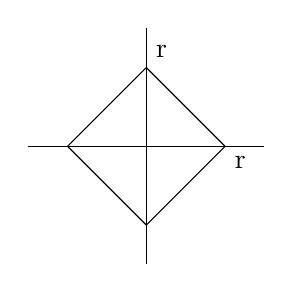
\begin{tikzpicture}	
		\draw (0,1.5) -- (0,-1.5);
		\draw (1.5,0) -- (-1.5,0);
		\draw (0,1) -- (-1,0) -- (0,-1) -- (1,0) -- cycle;
		\draw (1,0) node[below right]{r};
		\draw (0,1) node[above right]{r};
		\end{tikzpicture}~\\
		\fbox{$||\textbf{x}|| = \somme{n}{i=1}{|x_i|}$}\\
		~\\
		$||\ \ ||_1$
	\end{center}
\end{multicols}
$n=1$ même chose a chaque fois\\
$n=2$ Soit \textbf{x} = $(x,y)$
\begin{enumerate}
	\item $|x| + |y| = \sqrt{x^2+y^2+2|x||y|} \geq \sqrt{x^2+y^2}$
	\item $\sqrt{2}\sqrt{x^2+y^2} = \sqrt{2x^2 + 2y^2} = \sqrt{(|x|+|y|)^2 + (|x|-|y|)^2}$
\end{enumerate}
Donc $\frac{1}{\sqrt{2}}(|x|+|y|) \leq \sqrt{x^2+y^2} \leq |x|+|y|$\\
$\frac{1}{\sqrt{2}}||\textbf{x}||_1 \leq ||\textbf{x}||_2 \leq ||x||_1$\\
$||\textbf{x}||_2:  \leq ||\textbf{x}||_1 \leq \sqrt{2}||\textbf{x}||_2$
\begin{boite}
	\evid{Définition :} Deux normes $||\ ||_a$ et $||\ ||_b$ sur un espace vectoriel sont dites équivalentes s'il existe des constantes $C_1,\ C_2 > 0$ telles que 
	\begin{equation*}
		C_1||\textbf{x}||_a \leq ||\textbf{x}||_b \leq C_2||\textbf{x}||_a
	\end{equation*}
	pour tous les éléments \textbf{x} de l'espace vectoriel.
\end{boite}
\begin{boite}
	\evid{Théorème :} Sur \rn toutes les normes sont équivalentes et en particulier on a pour tout \textbf{x}$\in$ \rn
	\begin{align*}
		\frac{1}{\sqrt{n}}||\textbf{x}||_1 \leq \text{\fcolorbox{red}{white}{$||\textbf{x}||_2 \leq ||\textbf{x}||_1$}}\\
		||\textbf{x}||_\infty \leq ||\textbf{x}||_2 \leq \sqrt{n}||\textbf{x}||_\infty
		\end{align*}
\end{boite}
\evid{Proposition 1.6} Soit ($\textbf{x}_k$) une suite dans \rn et \textbf{a}$\in \rn$. Alors 
\begin{equation*}
	\limite{k\to\infty}\textbf{x}_k = \textbf{a} \iff \limite{k\to\infty}\textbf{x}_{k,i} = \textbf{a}_i \qquad i = 1,\ldots,n
\end{equation*}
où $(\textbf{x}_k) = (x_{k,i},\ldots,x_{k,n}) \quad , \quad \textbf{a} = (a_1,\ldots,a_n)$\\
\evid{Démonstration :}\\
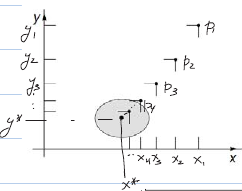
\includegraphics[scale=0.5]{images/demonstration}\\
\underline{n=2 :} \enquote{$\to$} on a $||\textbf{x}_k - \textbf{a}|| = \sqrt{(x_{k,1} - a_1)^2 + (x_{k,2} -a_2)^2}$\\
et donc $|x_{k,1}-a_1| \leq ||\textbf{x}_k - \textbf{a}|| \to (k\to\infty) \to 0$\\
(pareil pour $x_{k,2}$)\\
\enquote{$\leftarrow$} on a (car $||\ ||_2 \leq ||\ ||_1$)\\
$||\textbf{x}_k - \textbf{a}|| \leq |x_{k,1} - a_1| + |x_{k,2} -a_2| \to (k\to\infty)\to 0$ (les deux tendent vers 0 a k vers infini)

\section[Chemin $\R \to \Rm$]{Chemins (courbes) dans $\Rm$ (fonctions de $\R\to\R^m$)}
\setcounter{equation}{0}
\subsection{Chemins dérivables}
\begin{boite}
	\evid{Définition :} Une fonction continue $f:\R\to\Rm$ est appelée un chemin
\end{boite}
\underline{Notation} : (\Rm comme espace vectoriel)
\begin{equation*}
	f(x) = \big(f_1(x), \ldots , f_m(x)\big)^T \qquad x\in\R
\end{equation*}
avec $f_i : \rtor \quad i=1,\ldots,m$\\
\underline{Remarque} Conséquence de Prop.1.6. $f$ continue $\iff f_i$ continue, $i=1,\ldots,m$
\begin{boite}
	\evid{Définition :} Soit $I\subset\R$ un intervalle ouvert. Une fonction $f:i\to\Rm$ est dérivable en $x_0 \in I$ si les $n$ fonctions $f_1,\ldots,f_m$ sont dérivables en $x_0$ et 
	\begin{equation*}
		f0(x_0) = f_1'(x_0),\ldots,f_m'(x_0) \qquad (\text{matrice } x\times 1)
	\end{equation*}
\end{boite}
\underline{Remarque :} On a 
\begin{align*}
	f'(x_0) = \limite{n\to0} \frac{1}{n}\big(f(x_0+h) - f(x_0)\big)\\
	= \limite{h\to 0}\Big(\frac{1}{n}\big(f_1(x_0+h)-f_1(x_0)\big) \ldots\frac{1}{n}\big(f_m(x_0+h)-f_m(x_0)\big)\Big)^T\\
	=\text{on distribue la limite sur les fractions, et on transpose le tout.}
\end{align*}
chaque partie "fraction" vaut la dérivée de $f_i(x)$

\evid{Interprétation :} Si on interprète $t \equiv x\in I$ comme le temps et $f(t)$ comme la position d'un objet dans \Rm ($m=3$ disons), alors $f'(t)$ est le vecteur de la vitesse instantanée de l'objet.\\
\begin{boite}
	\evid{Définition :} Un point $t$ ou $f'(x) = 0$ est appelé un point stationnaire (ou singulier) du chemin (différentiable) $f$
\end{boite}

\evid{Exemples :}
\begin{enumerate}[label=\roman*)]
	\item $I = [0,2\pi],\ r>0,\quad t\to (r\cos(t),r\sin(t))^T = f(x) \in \R^2$ %{trou image cercle téléphone}
	\begin{boite}[0.7]
		\evid{Définition :} L'image de $f$ est appelée la trace du chemin	
	\end{boite}
	On a $f'(t) = (-r\sin(t), r\cos(t))^T \in \R^2$\\
	$||f'(t)|| = r$\\
	Longueur du chemin pour un tour : $\intt{2\pi}{0}{||f'(t)||} = \intt{2\pi}{0}{r} = 2\pi r$
	\item Soit $f:I\to \R,\quad I = [a,b]$ une fonction dérivable. Le graph de g\\
		$T_g:=\{(x,y) \in \R^2 : y=g(x)$ pour un $x\in I\}$\\
		%{trou graph, pas photographié}\\
		Ce graph est la trace du chemin $f:I\to\R^2$\\
		$x\to\big(x,g(x)\big)^T =:f(x)$\\
		On a $f'(x) = (1,g'(x))^T,||f'(x)|| = \sqrt{1+g'(x)^2}$\\
		Donc $l = \intx{b}{a}{\sqrt{1+g'(x)^2}}$ est la longueur du graph de g
	 \item Soit $r>0 \ , \ c\in\R$ et soit $f: \R\to\R^3$ définie par :\\
		 \begin{multicols}{2}
		 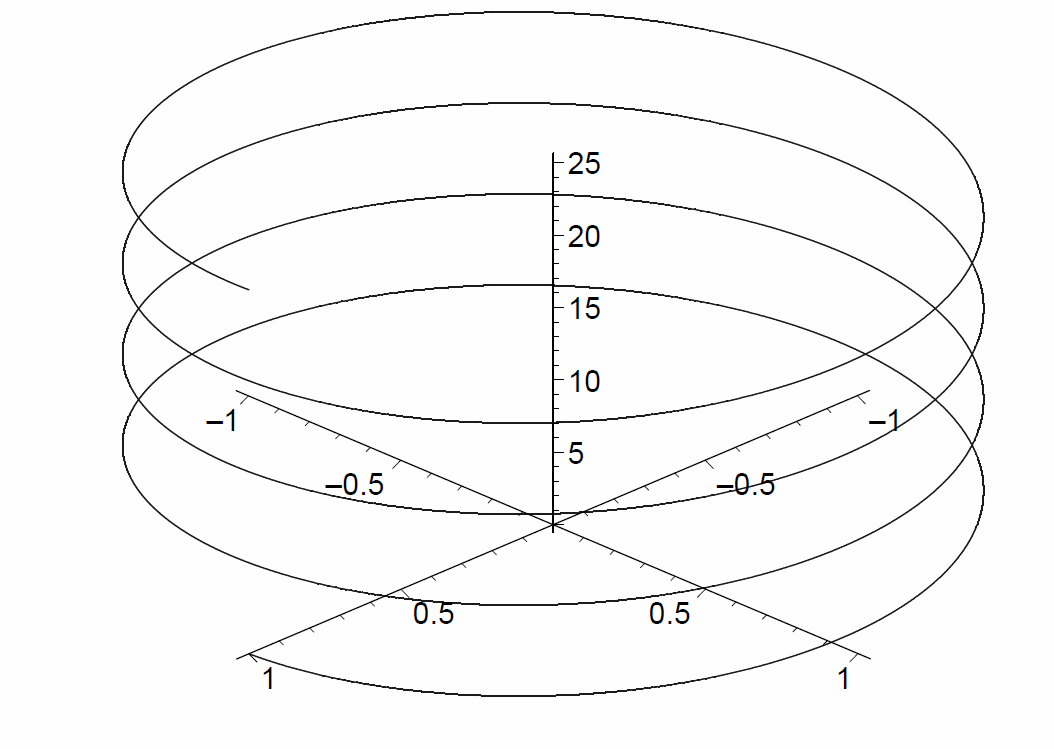
\includegraphics[scale=0.2]{images/spirale}  
		 \columnbreak		 
		\begin{center}
		 	$t\to f(t) = 
		 	\begin{pmatrix}
			 	r\cos(t)\\
			 	r\sin(t)\\
			 	ct
		 	\end{pmatrix}$
		 	$f'(t) =
		 	\begin{pmatrix}
			 	-r\sin(t)\\
			 	r\cos(t)
			 	c
			 \end{pmatrix}$\\
			 $||f'(t)|| = \sqrt{r^2+c^2}$
		 \end{center}		 
		 \end{multicols}
		 Longueur d'un tour de la spirale : $\intt{2\pi}{0}{||f'(t)||} = \sqrt{r^2+c^2}\cdot 2\pi$
	 \item Soit $f: \R\to\R^2$ définie par 
		 \begin{equation*}
			 t\to f(t) = \begin{pmatrix}
					 t^2-1\\
					 t^3-t
			 \end{pmatrix}
		 \end{equation*}
		 On a $f(-1) = f(1) = \begin{pmatrix}
		 0\\
		 0
		 \end{pmatrix}$ (f n'est pas injective)\\
		 \begin{multicols}{2}		 
		 \begin{center}
		 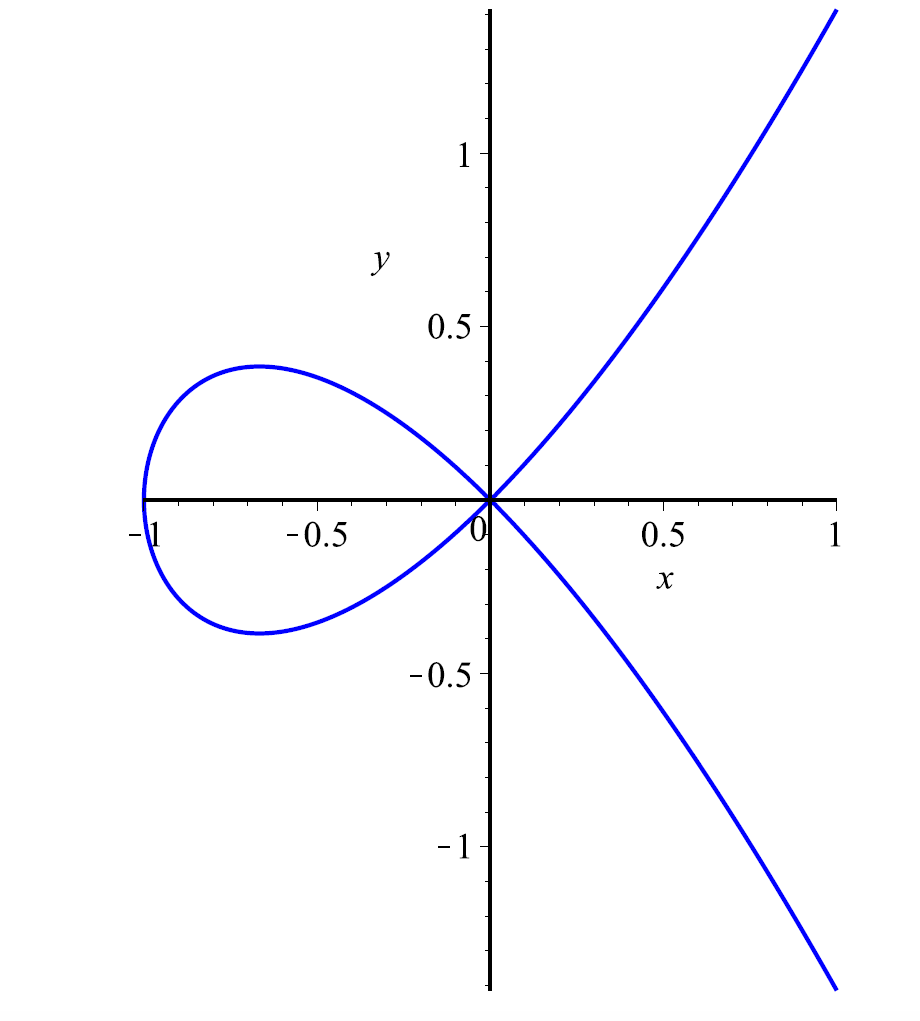
\includegraphics[scale=0.2]{images/loop}
		 on a $f'(t) = \begin{pmatrix}
		 	2t\\
		 	3t^2-1
		 \end{pmatrix}$~\\
		  ~\\
		 $f'(-1) = \begin{pmatrix}
		 	-2\\
		 	2
		 \end{pmatrix}, f'(1) = \begin{pmatrix}
		 	2\\
		 	2
		 \end{pmatrix}$\\
		 et $||f'(t)|| = \sqrt{9t^4-2t^2 + 1}$
 		 \end{center}
		 \underline{Remarque :}\\
		 $\left< f'(-1), f'(1)\)> (=0) = \\
		 ||f'(1)||\cdot||f'(-1)||(=\sqrt{8} chacun)\cos(\theta)$
		 \end{multicols}
\end{enumerate}
\section{Fonctions de \rn}
\setcounter{equation}{0}
\subsection{Introduction (n=2), définitions}
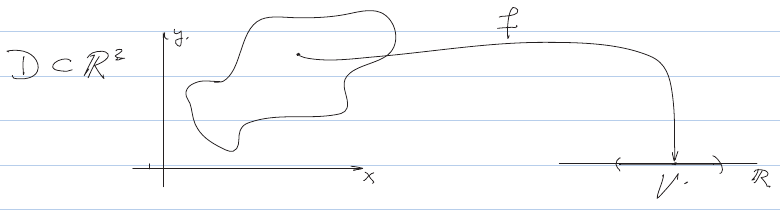
\includegraphics[scale=0.5]{images/fonction_deux_variables}\\
$f:D\to \R$, D le domaine de définition de f\\
$(x,y) \to f(x,y)$ V l'image de F\\
$V = \{z\in \R : z = f(x,y)$ pour un $(x,y)\in D\}$\\
$x,y$ les variables indépendantes, $z$ la variable dépendante.\\
Le graph de $f$ est une surface :\\
$T_f := \{x,y,z)\in\R^3 : (x,y) \in D \ , \ z = f(x,y)$\}\\
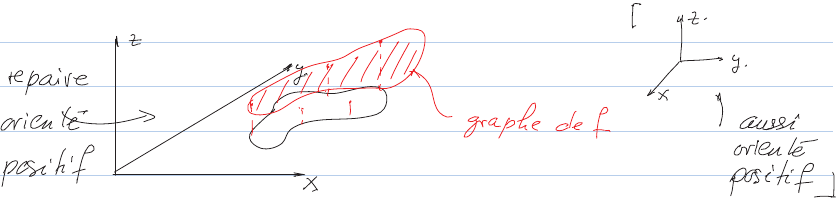
\includegraphics[scale=0.5]{images/repere_oriente_positif}\\
\underline{Exemple 1} \\
$D = \{(x,y) \in \R^2 \ : \ x^2+y^2 \leq 1\}$\\
$f:D\to \R \ , \ f(x,y) = \sqrt{1-x^2-y^2}$\\
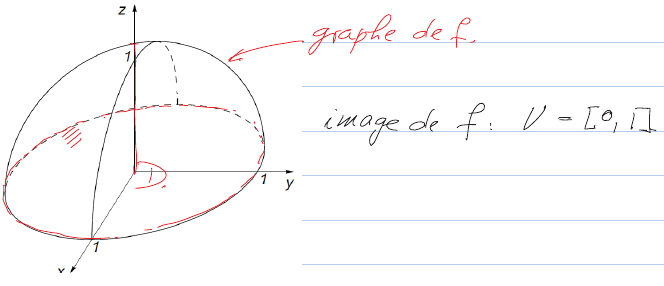
\includegraphics[scale=0.5]{images/demi_sphere}\\
\underline{Exemple 2 :} (important !!!!!!!!!!!!!!!)\\
$f:\R^2 \to \R, \ f(x,y) = ax+by+c$ avec $a,b,c \in \R$ donnés.
\begin{enumerate}[label=\roman*)]
	\item $a \neq 0$ ou $b\neq 0 \qquad$ l'image de f = \R
	\item $a=b=0 \qquad$ l'image de f = $\{c\}$\\
	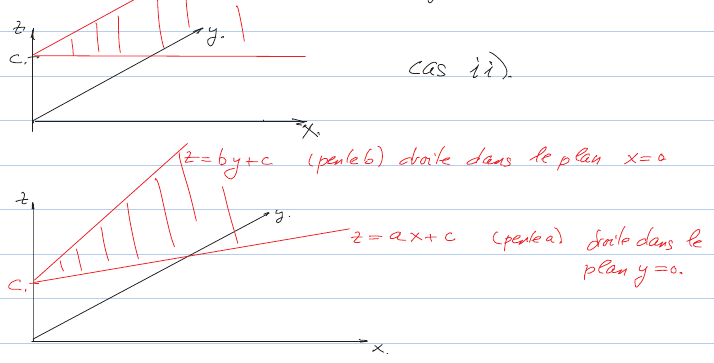
\includegraphics[scale=0.5]{images/deux_droites}
\end{enumerate}
\newpage
\begin{multicols}{2}
	\underline{Exemple 3}\\
	$f : D \to \R \quad, D = \{(x,y) \in \R^2 : x^2 < y\}$ . La partie grise est notre domaine de définition. Sur celui-ci nous plaçons une fonctions :\\
	$f(x,y) = \frac{x\cdot y - 1}{\sqrt{y-x^2}}$\\
	Image de $f = \R$\\
	Coupe à $y = 1 : \quad z = f(x,1) = \frac{x-1}{\sqrt{1-x^2}} \underset{\substack{x\to 1 \\ x<1}}{\to} 0$ (voir fichier Maple 001)
	\columnbreak
	
	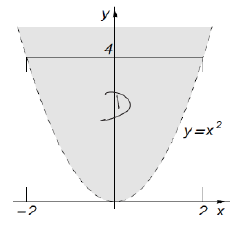
\includegraphics[scale=0.5]{images/parabole_grise}\\
	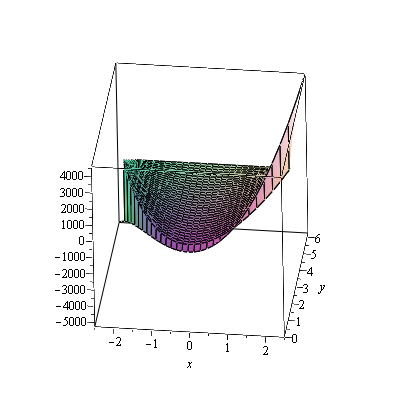
\includegraphics[scale=0.5]{images/maple001}
		\end{multicols}

\begin{boite}
	\evid{Définition :}(ensemble de niveau)\\
	Soit $f: D\to \R$ avec $D\subset \rn$ le domaine de définition de $f$. Soit $c\in \Im(f) \subset \R$
	\begin{equation*}
		N_f(c) := \{\textbf{x} \in D : f(\textbf{x}) = c\} \subset D
	\end{equation*}
	est appelé l'ensemble de niveau de $f$ pour $c$.
\end{boite}
\underline{Notation :} $N_f(c),\quad f^{-1}(c) := \{\textbf{x} \in D(f) : f(\textbf{x}) = c\}$\\
\evid{Exemples :} n=1 (trou dessin)\\
n=2 retour aux exemples 1-3\\
\underline{Pour exemple 1 :}\\
$f(x,y) = \sqrt{1-x^2-y^2}\\
D = \{(x.y) \in \R^2 : x^2+y^2 \leq 1\}\\
\Im(f) = [0,1] \ni c$\\
$N_f(c) = \{(x,y) \in D : \sqrt{1-x^2-y^2} = c\} \iff 1-x^2-y^2=c^2 \iff x^2+y^2 = 1-c^2$ (un cercle de rayon $(\sqrt{1-c^2}$)

\underline{Pour exemple 2}\\
$f: \R^2 \to \R \ , \ D = \R^2 \ , \ f(x,y) = ax+by+c$ avec $a,b,c \in \R$ donnée.
\begin{enumerate}
	\item $a=b=0 \ , \ \Im(f) = c \quad N_f(c)  = \R^2$
	\item $a\neq 0$ ou $b\neq 0 \ , \ \Im(f) = \R$. Soit $c^* = \Im(f)$\\
	$N_f(c^*) = \{(x,y) \in \R^2 : ax+by+c = c^*\}$ (des droites dans $\R^2= D$)
\end{enumerate}

\underline{Pour l'exemple 3} $D = \{(x,y) \in \R^2 : x^2<y\}$ \\
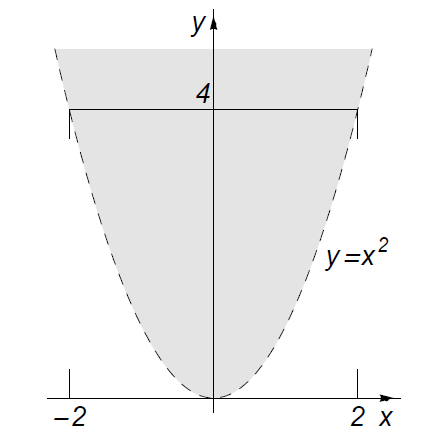
\includegraphics[scale=0.3]{images/domaine_parabole}
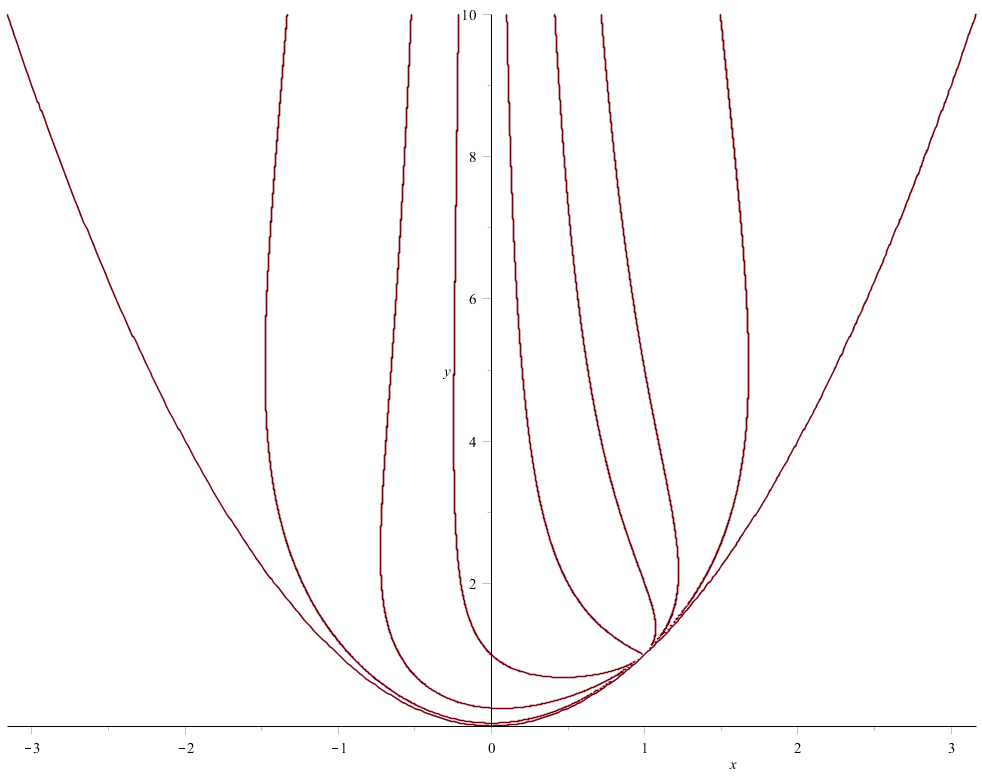
\includegraphics[scale=0.2]{images/onion}

\subsection{Limites et continuité}
\evid{Voir le chapitre 1 pour les définitions}\\
\evid{Exemple 1 :} (opérations algébriques)
\begin{enumerate}
\item  Soit $f : \R^2 \to \R \ , \ (x,y) \to f(x,y) = x+y$\\
$\llimite{(x,y) \to (x^*,y^*)}{(x,y) \neq (x^*,y^*)}{(x+y)} = x^* + y^*$\\
car $|(x+y) - (x^*+y^*)| \leq \underbrace{\underbrace{|x-x^*|}_{\to 0} + \underbrace{|y-y^*|}_{\to 0}}_{\text{lorsque } (x,y) \to (x^*,y^*)} \to 0$\\
Donc $f$ continue sur $\R^2$
\item Soit $f: \R^2 \to \R \ , \ (x,y) \to f(x,y) = xy$\\
f est continue en tout point $(x^*,y^*) \in \R^2$ car\\
$\llimite{(x,y) \to (x^*,y^*)}{(x,y) \neq (x^*,y^*)}{f(x,y)} = f(x^*,y^*)$
\end{enumerate}
\underline{Démonstration :} $|xy - x^*y^*| = |(x-x^*)y + x^*(y-y^*)| \leq |x-x^*||y| +|x^*||y-y^*|$ (borné pour toute suite $y_n, y_n\neq y^* \ , \ \limite{\ninf} y_n = y^*$)\\
 $|\underbrace{x-x^3}_{\to 0}| M + |x^*||\underbrace{y-y^*}_{\to 0}| \to 0$\\
 \begin{boite}
	$\to$ continuité des fonctions polynômes de deux (ou plusieurs) variables, ainsi que la continuité des fonctions rationnelles sur leur domaine de définition.	
\end{boite}

\evid{Exemple 2}\\
$f(x,y) = \frac{x^2-y^2}{x^2+y^2} \ , D(f) = \R^2\setminus \{0,0\} \equiv D$\\
Par exemple 1, $f$ est continue sur D ($f$ est une fonction rationnelle)\\
$\llimite{(x,y) \to (0,0)}{(x,y) \neq (0,0)}{f(x,y)}$ n'existe pas\\
car sur toute suite de la forme $(x_n, 0)$ avec $\limite{\ninf} x_n = 0$ on a 
\begin{equation*}
f(x_n, 0) = \frac{x_n^2 - 0^2}{x_n^2+0^2} = 1
\end{equation*}
Par contre, sur toute suite de la forme $(0,y_n),\limite{\ninf}y_n = 0$ on a 
\begin{equation*}
	f(0,y_n) = \frac{0^2-y_n^2}{0+y_n^2} = -1
\end{equation*}
Comme ces deux limites ne sont pas identiques, la limite n'existe pas.

\evid{Exemple 3}\\
$f(x,y) = \frac{xy}{x^2+y^2}, D(f) = \R^2\setminus \{0,0\} \equiv D$\\
$f$ est continue sur D (car rationnelle)\\
Sur $(x_n,0)$ on a $f(x_n,0) = \frac{x_n 0}{x_n^2 + 0^2} = 0$\\
Sur $(0,y_n)$ on a $f(0,y_n) = \frac{0 y_n}{0+y_n^2} = 0$\\
Mais sur une suite de la forme $(x_n,x_n)$ on a 
\begin{equation*}
	f(x_n,x_n) = \frac{x_n x_n}{x_n^2+x_n^2} = \frac{1}{2} \neq 0
\end{equation*}
Donc $f$ n'a pas de limite en $(0,0)$\\
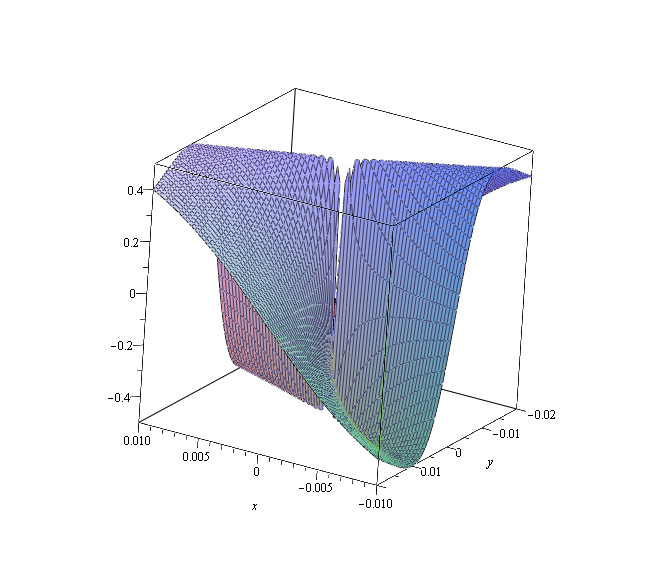
\includegraphics[scale=0.3]{images/sanslimite}

\evid{Exemple 4}\\
$f(x,y) = \frac{x^2y}{x^2+y^2} \ D(f) = \R^2 \setminus \{0,0\} \equiv D$\\
on a  $\llimite{(x,y) \to (0,0)}{(x,y) \neq (0,0)}{f(x,y)} = 0$\\
\underline{Démonstration} Coordonnées polaires (comme en TikZ, mais on considère $\R^2\setminus\{(0,0)\}$)\\ 
\begin{wrapfigure}[3]{r}{2cm}
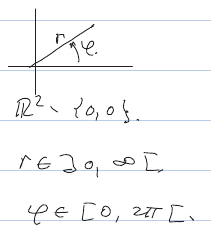
\includegraphics[scale=0.5]{images/polaire}
\end{wrapfigure}
$(x,y)$ s'exprime en une et une seule coordonnée $(r,\varphi)$\\
on a que $r_n = \sqrt{x_n^2+y_n^2} \underset{{\substack{(x_n,y_n) \to (0,0) \\ (x_n,y_n) \neq (0,0)}}}{\longrightarrow} 0$\\
Donné une suite $(r_n, \varphi_n) \ , \ r_n \underset{\ninf}{\to} 0 \ ,$ \fbox{$x_n = r_n \cos(\varphi_n) \ , \ y_n = r_n \sin(\varphi_n)$}\\
$|f(x_n,y_n)| = |\frac{r_n^3\cos(\varphi_n)^2\sin(\varphi_n)}{r_n^2}| \underbrace{<}_{\text{indépendant de }\varphi_n} r_n \underset{\ninf}{\longrightarrow} 0$ 

\begin{boite}
	\evid{Prolongement par continuité}\\
	La fonction 
	\begin{equation*}
		\overset{~}{f}(x,y) = \left\{\begin{array}{ll}
		\frac{x^2y}{x^2+y^2} & \text{pour } (x,y) \neq (0,0)\\
		0 & \pour (x,y) = (0,0)
		\end{array}\right.
	\end{equation*}
	est continue sur $\R^2$
\end{boite}

\evid{Exemple 5} $\qquad \R^2\setminus\{(0,0)\} \ni (x,y) \iff (r,\varphi) \in \R^*_+ \times [0,2\pi[$\\
$f : \R^2 \setminus \{(0,0)\} \to \R\\
f(x,y) = \left\{\begin{array}{ll}
\frac{r}{\varphi} & \varphi \in ]0,2\pi[\\
0 & \varphi = 0
\end{array}\right.$\\
$\llimite{r\to 0}{r>0}{f(x,y)} = \llimite{r\to 0}{r>0}{\frac{r}{\varphi}} = 0$\\
$\llimite{r\to 0}{\varphi = 0}{f(x,y)} = \llimite{r\to 0}{\varphi = 0}{0} = 0$\\
Il faut contrôler toutes les suites (dessin graphe/coquillage)\\
La limite n'existe pas, car pour(une suite de la forme $(R_n, \varphi_n = r_n) \ , \ r_n > 0 \ , \ r_n \underset{n\to\infty}{\longrightarrow}$ on a
\begin{align*}
	x_n = r_n \cos(\varphi_n) \underset{\text{grand}}{=} r_n + o(r_n^3)\\
	y_n = r_n \sin(\varphi_n) \underset{\text{grand}}{=} r_n(r_n+o(r_n^2)) = r_n^2 + o(r_n^3)
\end{align*}

Donc $<_n = x_n^2 + o(x_n^3)$ (petit dessin)\\
On a $f(x_n,y_n) = \frac{r_n}{\varphi_n} = \frac{r_n}{r_n} = 1 \underset{\ninf}{\longrightarrow} 1$
Voir série 5

\subsection{Dérivées partielles, Dérivée, Fonctions de classe $C^1$}
\subsubsection{Dérivées partielles (fonctions dérivables)}
\evid{3.3.1.1 Définitions}
\begin{boite}
	\underline{Terminologie}\\
	Existence des dérivées partielles\\
	$\iff$ Fonctions différentiables\\
	$\iff$Fonctions dérivables
\end{boite}

\begin{boite}
	 \underline{Remarque :} Pour pouvoir définir les dérivées partielles correctement, il est indispensable de préciser les noms des variables
\end{boite}

\begin{boite}
	\underline{Définition :}\\
	La dérivée partielle d'une fonction de plusieurs variables est la dérivée par rapport à \textit{une} des variables, les autres variables étant gardées constantes.
\end{boite}
\begin{boite}[1]
	\underline{Définition explicite pour le cas $n=2$}\\
	Soit $f : D\to \R,\ (\textcolor{red}{x},\textcolor{blue}{y}) \to f(\textcolor{red}{x},\textcolor{blue}{y}),\ (x_0,y_0) \in D$ où $D\subset \R^2$ ouvert. La dérivée partielle de f en $(x_0,y_0)$ par rapport à la variable \textcolor{red}{$x$} est le nombre
\begin{equation*}
\underbrace{\frac{\delta f}{\delta \textcolor{red}{x}} (x_0,y_0)}_{\in \R} = \limite{h\to 0} \frac{f(x_0+h,y_0) - f(x_0,y_0)}{h}
\end{equation*}
la dérivée partielle de $f$ en $(x_0,y_0)$ par rapport à la variable \textcolor{blue}{y} est le nombre
\begin{equation*}
	\underbrace{\frac{\delta f}{\delta \textcolor{blue}{y}} (x_0,y_0)}_{\in \R} = \limite{h\to 0} \frac{f(x_0,y_0+h) - f(x_0,y_0)}{h}
\end{equation*}
\end{boite}
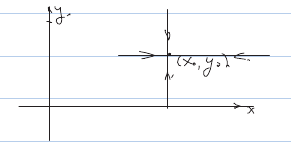
\includegraphics[scale=0.5]{images/deriv_part}\\
$h'(y_0) = \frac{\delta f}{\delta y}(x_0,y_0)\\
g'(x_0,y_0) = \frac{\delta f}{\delta x}(x_0,y_0)$
\begin{boite}[0.7]
\evid{Notations :}\\
$\frac{\delta f}{\delta x} (x_0,y_0)\, \delta x f(x_0),\ f_x'(x_0,y_0),\ f_x(x_0,y_0),\ D_xf(x_0,y_0),\\ \delta_1 f(x_0,y_0),\ D_1 f(x_0,y_0)$\\
(pareil avec y, remplacement de x par y et de 1 par 2)
\end{boite}
\begin{boite}
	\underline{Définition (n général)} Soit $f:D\to \R,\ \textbf{x} \to f(\textbf{x)},$ pour $\textbf{x} = (x_y,\ldots,x_n) \in D$ où $D\subset \R^n$ est ouvert. La dérivée partielle de $f$ en $\textbf{x}_0\in D$ est le nombre 
	\begin{equation*}
	\frac{\delta f}{\delta \textcolor{red}{x}_k} (\textbf{x}_0) = \limite{h\to 0} \frac{f(\textbf{x}_0 + e_k h)-f(\textbf{x}_0)}{h}
	\end{equation*}
	où $e_k = (0,\ldots,1,0,\ldots,0)^T$ est le k\ts{ème} vecteur de la vase canonique de $\R^n$
\end{boite}
\begin{boite}
	$\frac{\delta f}{\delta x_k}(\textbf{x}_0),\ \delta_{x_k} f(\textbf{x}_0),...$
\end{boite}
\evid{3.3.1.2 Interprétation géométrique} (dessin pour n=2)\\
La dérivée partielle $\frac{\delta f}{\delta x}(x_0,y_0)$ est la pente de la tangente au graphe de la fonction $z=g(x) = f(x,y_0)$ en $(x_0,y_0,z_0)$ où $z_0 = f(x_0,y_0)$, et $\frac{\delta f}{\delta y}(x_0,y_0)$ est la pente de la tangente au graphe de la fonction $z= h(x) = f(x_0,y)$ en $(x_0,y_0,z_0)$\\
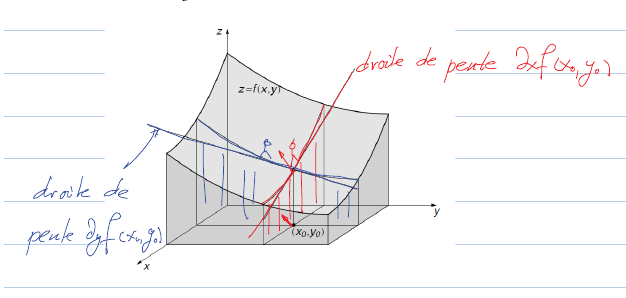
\includegraphics[scale=0.9]{images/interpret_geom}\\
\evid{3.3.1.3  Le gradient}\\
\begin{boite}
	\underline{Définition :}\\
	Soit $f:D\to \R, \textbf{x} \to f(\textbf{x}),\ \textbf{x} = (x_1,\ldots,x_n) \in D$ où $D \subset \R^n$ est ouvert, et soit $\textbf{x}_0 \in D$ le vecteur 
	\begin{equation*}
		\nabla f(\textbf{x}_0) \equiv \text{grad}\underbracket{\ } f(x_0) \( \frac{\delta f}{\delta x_1}(\textbf{x}_0),\ldots, \frac{\delta f}{\delta x_n}(\textbf{x}_0)\)^T
	\end{equation*}
	est appelé le gradient de f en $\textbf{x}_0$
\end{boite}
\underline{Représentation graphique du gradient :}\\
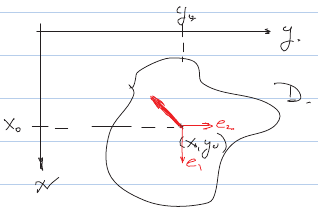
\includegraphics[scale=0.9]{images/gradient_graph}\\ 
$<e_1,e_2> = \R^2$ l'espace vectoriel attaché en ($x_0,y_0)$\\
Le gradient indique \underline{dans le domaine de définition} de f la direction de la pente la plus forte (positive)\\
\evid{3.3.1.4 Les fonctions dérivées partielles}\\
\begin{boite}
	\underline{Définition ($n=2$)} Soit $f:D\to \R,\ (x,y) \to f(x,y)$ ou $D\subset \R^2$ est ouvert. Si les dérivées partielles $\frac{\delta f}{\delta x} (x_0,y_0)$ et $\frac{\delta f}{\delta y}(x_0,y_0)$ existent pour tout $(x_0,y_0) \in D$. On peut définir des (nouvelles) fonctions
	\begin{align*}
		\frac{\delta f}{\delta \textcolor{red}{x}} : D\to \R,\ (x,y) \to \frac{\delta f}{\delta \textcolor{red}{x}}(x,y)\in \R = \llimite{h\to 0}{h\neq 0}{...}\\
		\frac{\delta f}{\delta \textcolor{blue}{y}} D\to\R,\ (x,y) \to \frac{\delta f}{\delta \textcolor{blue}{y}} (x,y) \in \R = \llimite{h\to 0}{n\neq 0}{...}
	\end{align*}
\end{boite}
\begin{boite}
	\underline{Terminologie :} Si les fonctions $\frac{\delta f}{\delta x},\ \frac{\delta f}{\delta y}$ existent, on dit que la fonctions f est \textit{partiellement différentiable} ou encore que f est \textit{dérivable}\\
	\fcolorbox{red}{white}{dérivable = partiellement différentiable}
\end{boite}
\begin{boite}
	\underline{Notation} \\
	$\frac{\delta f}{\delta x}, \delta_x, f'(x),...$
\end{boite}
\evid{Exemple :} Soit $f: \R^2 \to \R,\ (x,y) \to f(x,y) = x^2-y^2$\\
Alors $\frac{\delta f}{\delta x} : \R^2 \to \R,\ (x,y) \to \frac{\delta f}{\delta x}(x,y) = 2x\\
\frac{\delta f}{\delta y} :  \R^2 \to \R,\ (x,y) \to \frac{\delta f}{\delta y}(x,y) = -2y$\\
Donc on a par exemple : $\frac{\delta f}{\delta x} (0,1) = 0,\ \frac{\delta f}{\delta y}(0,1) = -2$\\
\underline{Test de compréhension :} Soit $f(x,y) = x^2-y^2$. Alors on peut s'amuser à définir la fonction 
\begin{equation*}
	g : \R^2 \to \R,\ (x,y) \to f(x,y) = \frac{\delta f}{\delta y}(y,y)
\end{equation*}
$g(x,y) = ?$\\
\evid{3.3.1.5 Deuxièmes dérivées partielles (n=2)}
\begin{boite}
	\evid{Définition :} Soit $f: D\to \R,\ (x,y) \to f(x,y),$ où $D\subset \R^2$ est ouvert. Pour chacune des fonctions
	\begin{align*}
		\frac{\delta f}{\delta x} : D\to \R\ , \ (x,y) \to \frac{\delta f}{\delta x} (x,y)\\
		\frac{\delta f}{\delta y} : D\to \R\ , \ (x,y) \to \frac{\delta f}{\delta y} (x,y)
	\end{align*}
	on peut étudier l'existence des dérivées partielles par rapport à $x$ et $y$ en ($x_0,y_0) \in D$ (calcul de limites). Si les nombres 
	\begin{align*}
	\frac{\delta \frac{\delta f}{\delta x}}{\delta x}(x_0,y_0) \ , \ \frac{\delta \frac{\delta f}{\delta x}}{\delta y}(x_0,y_0)\\
	\frac{\delta \frac{\delta f}{\delta y}}{\delta x}(x_0,y_0) \ , \ \frac{\delta \frac{\delta f}{\delta y}}{\delta y}(x_0,y_0)
	\end{align*}
	Existent pour tout $(x_0,y_0) \in D$ on peut définir les fonctions des deuxièmes dérivées partielles 
	\begin{equation*}
		\frac{\delta^2 f}{\delta x^2},\frac{\delta^2 f}{\delta y \delta x},\ \frac{\delta^2 f}{\delta x \delta y},\ \frac{\delta^2 f}{\delta y^2}
	\end{equation*}
	par les équations 
	\begin{align*}
		\frac{\delta^2 f}{\delta x^2} (x_0,y_0) = \frac{\delta \frac{\delta f}{\delta x}}{\delta x}(x_0,y_0)\Bigg( := \llimite{h\to 0}{h\neq 0}{\frac{\frac{\delta f}{\delta x} (x_0+h, y_0) - \frac{\delta f}{\delta x} (x_0,y_0)}{h}}\Bigg)\\
		\frac{\delta^2 f}{\delta y \delta x } (x_0,y_0) = \frac{\delta \frac{\delta f}{\delta x}}{\delta y}(x_0,y_0)\Bigg( := \llimite{h\to 0}{h\neq 0}{\frac{\frac{\delta f}{\delta x} (x_0, y_0+h) - \frac{\delta f}{\delta x} (x_0,y_0)}{h}}\Bigg)\\
		\frac{\delta^2 f}{\delta x \delta y} (x_0,y_0) = \frac{\delta \frac{\delta f}{\delta x}}{\delta x}(x_0,y_0)\Bigg( := ...\Bigg)\\
		\frac{\delta^2 f}{\delta x \delta y} (x_0,y_0) = \frac{\delta \frac{\delta f}{\delta x}}{\delta x}(x_0,y_0)\Bigg)
	\end{align*}
\end{boite}
\begin{boite}
	\underline{Remarque :} Souvent on écrit directement $\frac{\delta^2 f}{\delta x^2}(x_0,y_0)$ au lieu de $\frac{\delta \frac{\delta f}{\delta x}}{\delta x}(x_0,y_0)$ pour la valeur de la dérivée partielle de la fonction $\frac{\delta f}{\delta x}$ par rapport à $x$ en $(x_0,y_0)$
\end{boite}
\begin{boite}
\underline{Notations :}\\
$\frac{\delta^2 f}{\delta x^2},\ \delta_x^2 f, \delta_1^2 f, D_1^2 f, D_{11} f, f_x...$
\end{boite}
\begin{boite}
\underline{Attention :} L'interprétation de $\frac{\delta^2 f}{\delta x\delta y}(x_0,y_0)$ varie d'un auteur à l'autre. L'ordre de $x$ et $y$ peut varier.\\
\underline{Heureusement :} On pour les fonctions de classe $C^2$ (à définir plus loin) que $\frac{\delta^2 f}{\delta x\delta y} = \frac{\delta^2 f}{\delta y \delta x}$
c'est à dire$\frac{\delta^2 f}{\delta x\delta y} (x_0,y_0) = \frac{\delta^2 f}{\delta y \delta x}(x_0,y_0)$\\
Mais voir la série 5
\end{boite}
\evid{3.3.1.6 : Dérivées partielles du deuxième ordre (n général)}\\
Soit $f: D\to R, \textbf{x} \to f(\textbf{x})$ avec $\textbf{x} = (x_1,..., x_n) \in D$ ou $D \subset \R^n$ est ouvert, et soient
\begin{equation*}
	\frac{\delta f}{\delta x_j} : D\to \R,\ \textbf{x}\to \frac{\delta f}{\delta x_j}(\textbf{x}),\ j=1,...,n
\end{equation*}
Les fonctions des deuxièmes dérivées partielles
\begin{equation*}
	\frac{\delta^2 f}{\delta x_i,\ \delta x_j} : D \to \R
	\end{equation*}sont définies en $\textbf{x}_0 \in D$ par les équations \\
	$\begin{array}{ll}
	\frac{\delta^2 f}{\delta x_i, \delta x_j}(\textbf{x}_0) & = \frac{\delta \frac{\delta f}{\delta x_j}}{\delta x_i}(\textbf{x}_0)\\
		& = \llimite{h\to 0}{h\neq 0}{\frac{\frac{\delta f}{\delta x_j}(\textbf{x}_0 + he_i - \frac{\delta f}{\delta x_j}(\textbf{x}_0)}{h}}
	\end{array}$ 	pour i=1,...,n
\begin{boite}
	Les deuxièmes dérivées partielles sont souvent arrangées dans un tableau (matrice $n\times n$)\\
	$\(\frac{\delta^2 f}{\delta x_i\delta x_j}\) = 
	\begin{pmatrix}
			\frac{\delta^2 f}{\delta x_1^2 }(\textbf{x}_0) & ... & \frac{\delta^2 f}{\delta x_1, \delta x_n}(\textbf{x}_0\\
			... & & ...\\
			\frac{\delta^2 f}{\delta x_n\delta x_1}(\textbf{x}_0) & .. & \frac{\delta^2 f}{\delta x_n^2} (\textbf{x}_0)
	\end{pmatrix}$\\
Qui est appelée la \underline{matrice Heissienne de f} : $Hess(f)(\textbf{x}_0)$
\end{boite}	

\begin{boite}
	\uline{Remarque :} $Hess(f)(\textbf{x}_0)$ peut être la transposée de cette matrice selon les auteurs\\
	\uline{Remarque :} Si f est suffisamment régulier (de classe $C^2$, voir plus bas), on a 
\begin{equation*}
	Hess(f)(\textbf{x}_0) = Hess(f)(\textbf{x}_0)^T
\end{equation*}
i.e. la matrice est symétrique
\end{boite}
\evid{3.3.1.7 Dérivées partielles d'ordre supérieur}\\
Par récurrence, on peut définir les dérivées partielles de tous les ordres\\
\underline{Exemple} $f: \R^2 \to \R,\ 8x.y) \to f(x,y)$\\
$\frac{\delta^3 f}{\delta x^3}(x_0,y_0) = \frac{\delta \frac{\delta^2 f}{\delta x^2}}{\delta x}(x_0,y_0) = \llimite{h\to 0}{h\neq 0}{\frac{\frac{\delta^2 f}{\delta x^2} (x_0 + h,y_0) - \frac{\delta^2f}{\delta x^2}(x_0,y_0)}{h}} \in \R$\\
\evid{3.3.1.8 Exemples}\\
\begin{multicols}{2}
\begin{enumerate}
	\item 	$f(x,y) = x^3y^2\\
			\frac{\delta f}{\delta x}(x,y) = 3x^2y^2\\
			\frac{\delta^2 f}{\delta x^2}(x,y) = 6xy^2\\
			\frac{\delta^3 f}{\delta y\delta x^2}(x,y) =$ {$12xy$}\\
			$\frac{\delta^2 f}{\delta y\delta x}(x,y) = 6x^2y\\
			\frac{\delta^3f}{\delta x \delta y \delta y}(x,y) = ${$12xy$}
			\columnbreak
			
	\item 	$f(x,y) = x^y \ , \ D = \{(x,y) \in \R^2,\ x>0\}\\
			\frac{\delta f}{\delta x}(x,y) = yx^{y-1}\\
			\frac{\delta f}{\delta y}(x,y) = x^y\ln(x)$
		\end{enumerate}
			\end{multicols}
\begin{enumerate}[resume]
	\item 	$f(x,y) = \left\{\begin{array}{lll}
			\frac{xy}{x^2+y^2} & \pour & (x,y) \neq (0,0)\\
			0 & \pour & (x,y) = (0,0)
			\end{array}\right.$\\
			f n'est pas continue en $(0,0)$	\\
			\underline{Pour $(x,y) \neq (0,0)$} (règles de calcul habituelles).\\
			$\frac{\delta f}{\delta x}(x,y) = \frac{y}{x^2+y^2} - \frac{2x^2y}{(x^2+y^2)^2}\\
			\frac{\delta f}{\delta y}(x,y)  = \frac{x}{x^2+y^2} - \frac{2xy^2}{(x^2+y^2)^2}$\\
			\underline{Pour $(x,y) = (0,0)$} (il faut utiliser les définitions !)\\
			$\frac{\delta f}{\delta x} (0,0) = \llimite{h\to 0}{h\neq 0}{\frac{(f(0+h, 0) - f(0,0)}{h}} = \llimite{h\to 0}{h\neq 0}{\frac{\frac{h0}{h^2+0^2} -0}{h}} = \llimite{h\to 0}{h\neq 0}{0} = 0$\\
			$\frac{\delta f}{\delta y} (0,0) = \llimite{h\to 0}{h\neq 0}{\frac{(f(0, 0+h) - f(0,0)}{h}} = \llimite{h\to 0}{h\neq 0}{\frac{\frac{0h}{0^2+h^2} -0}{h}} = \llimite{h\to 0}{h\neq 0}{0} = 0$
\end{enumerate}
\subsubsection{Fonctions différentiables}
\begin{boite}
	\evid{Rappel :}\\
	Définition de la dérivabilité et de la différentiabilité pour une fonction $f:I\to \R$ en $x_0 \in I,\ I$ un intervalle ouvert de \R\\
	\underline{Dérivable}
	\begin{equation}
		f'(x_0)  = \llimite{h\to 0}{h\neq 0}{\frac{f(x_0 + h) - f(x_0)}{h}}
		\label{derivable}
	\end{equation}
	existence de la limite\\
	\underline{Différentiable} 
	\begin{equation}
		f(x_0+h) = f(x_0) + \overbrace{a}^{\mathclap{\text{une matrice 1x1}}}h + r(x_0 + h) |h|
		\label{differentiable}
	\end{equation}
	existence d'un nombre $a\in \R$ tel que $\llimite{h\to 0}{h\neq 0}{r(x_0+h) = 0}$
\end{boite}
\evid{Remarques :}\\
$~\eqref{differentiable} \to \llimite{h\to 0}{h\neq 0}{f(x_0+h)} = f(x_0)$ donc différentiable $\to$ continue\\
$~\eqref{differentiable} \to \frac{f(x_0+h) - f(x_0)}{h} = a + r(x_0+h)\frac{|h|}{h} \underset{h\to 0, h\neq 0}{\longrightarrow} a$\\
Donc $~\eqref{differentiable} \to ~\eqref{derivable}$ avec $f'(x_0) = a$\\
$~\eqref{differentiable} \to \frac{f(x_0+h) - f(x_0) - ah}{|h|} = r(x_0 + h) \underset{h\to 0, h\neq 0}{\longrightarrow} 0$\\
\begin{boite}
	\evid{Définition :} Soit $f:D\to \R,\ \textbf{x} \to f(\textbf{x}),\ \textbf{x} = (x_1,...,x_n) \in D$ ou $D \subset \R^n$ est ouvert. La fonction est différentiable en $\textbf{x}_0 \in D$ s'il existe une matrice A $1\times n$ telle que
	\begin{equation*}
		f(\textbf{x}_0 + \textbf{h}) = f(\textbf{x}_0) + A\textbf{h} + r(\textbf{x}_0 + \textbf{h}) \cdot ||\textbf{h}||
	\end{equation*}
	telle que $\llimite{\textbf{h} \to 0}{\textbf{h} \neq 0}{r(\textbf{x}_0 + \textbf{h})}  =0$
\end{boite}
\begin{boite}
	\underline{Notation} : dans ce cours, on écrira $f'(\textbf{x}_0)$ pour la matrice A
\end{boite}
\begin{boite}
	\underline{Terminologie} $f'(\textbf{x}_0)$ est appelée la dérivée (totale) de $f$ ou encore la différentielle de $f$
\end{boite}
\begin{boite}
	Remarque : $~\eqref{differentiable}\iff$ existence d'une matrice $1 \times n\ f'(x_0)$ telle que 
	$\llimite{\textbf{h}\to 0}{\textbf{h}\neq 0}{\frac{f(\textbf{x}_0 + h) - f(\textbf{x}_0) - f'(\textbf{x}_0)\textbf{h}}{||\textbf{h}||}}$
\end{boite}
\begin{boite}
\underline{Proposition :} (différentiable $\to$ continue, existence des dérivées partielles)\\
Soit $f: D\to \R,\ \textbf{x} = f(\textbf{x}), \textbf{x} = x_1m...x_n) \in D$ ou $D \subset \R^n$ est ouvert, différentiable en $\textbf{x}_0$. Alors :
	\begin{enumerate}
		\item 	$f$ est continue en $\textbf{x}_0$
		\item 	$\frac{\delta f}{\delta x_k}(\textbf{x}_0)$ existent, $k=1,...,n$ et $f'(\textbf{x}_0) = \big(\frac{\delta f}{\delta x_1}(\textbf{x}_0),...,\frac{\delta f}{\delta x_n}(\textbf{x}_0)\big)$
	\end{enumerate}
\end{boite}
\evid{Démonstration :}
\begin{itemize}%[label=\roman*)]
	\item 	$~\eqref{differentiable} \to  \llimite{\textbf{h}\to 0}{\textbf{h} \neq 0}{f(\textbf{x}_0 + \textbf{h})} = f(\textbf{x}_0)$
	\item 	$~\eqref{differentiable} \underbrace{\to}_{\underbrace{\textbf{h}}_{\in \R^n}} = \underbrace{h}_{\in \R} e_k f(\textbf{x}_0 + he_k) = f(\textbf{x}_0) + hAe_k + r(\textbf{x}_0 + he_k)h$ \\%a corriger
			donc $\underbrace{\llimite{h\to 0}{h\neq 0}{\frac{f(\textbf{x}_0 + he_k) - f(\textbf{x}_0)}{h}}}_{= \frac{\delta f}{\delta x_k}(\textbf{x}_0)} = Ae_k = f(\textbf{x}_0) e_k$\\
\end{itemize}
\begin{boite}
Notation : 
$f'(\textbf{x}_0),\ d_{\textbf{x}_0}f,\ \nabla f(\textbf{x}_0)^T,... f'(\textbf{x}_0) \textbf{h},\ d_{\textbf{x}_0} f(\textbf{h}),\ \left< \nabla f(\textbf{x}_0), \textbf{h}\)>$
\end{boite}
\begin{boite}
	\evid{Remarque :} L'exemple 3 du chapitre 3.3.1.8 montre que l'existence des dérivées partielles 
	\begin{equation*}
		 \frac{\delta f}{\delta x_k}(\textbf{x}_0) \ , \ k=1,...,n
	\end{equation*}
	ne suffit pas pour garantir la différentiabilité en nu point $\textbf{x}_0$. Dans l'exemple, $f$ n'est même pas continue en $\textbf{x}_0$
\end{boite}
\begin{boite}
	\evid{Théorème :} Toutes les fonctions rationnelles sont différentiables sur leur domaine de définition
\end{boite}
\subsubsection*{Comment contrôler la différentiabilité d'une fonction dans le cas général ?}
\begin{enumerate}[label=\Alph*.]
	\item Méthode directe :\\
	$f(x,y) = \left\{ \begin{array}{lll}
		\frac{x^2y^2}{x^2+y^2} & \pour & (x,y) \neq (0,0)\\
		0 & \pour & (x,y) = (0,0)
	\end{array}\right.\\
	\underline{(x_0,y_0) \neq (0,0)}$\\
	$f$ est différentiable car $f$ est une fonction rationnelle sur$\R^2 \setminus \{(0,0)\}$ (dessin maple vallée)\\
	$\underline{(x_0,y_0) = (0,0)}$\\
	
	\begin{enumerate}%[label=\arabic*)]
		\setcounter{enumi}{-1}
		\item 	$f$ est continue en $(0,0)$ (une condition nécessaire à la différentiabilité)\\
				Pour $\rho > 0$ on a en coordonnées polaires :\\
				$| f(\rho \cos(\varphi), \rho \sin(\varphi)| \leq \rho^2 \to (\rho \to 0, \rho > 0) 0 = f(0,0)$
		\item f est partiellement différentiable = est dérivable\\
		$\frac{\delta f}{\delta x}(0,0) = \llimite{h\to 0}{h\neq 0}{\frac{\frac{0}{h^2} - 0}{h}} = 0\\
		\frac{\delta f}{\delta y}(0,0) = \llimite{h\to 0}{h\neq 0}{\frac{\frac{0}{h^2} - 0}{h}} = 0\\
		$ Donc si $f$ est différentiable en (0,0), on a \\
		$f'(0,0) = (\frac{\delta f}{\delta x}(0,0) , \frac{\delta f}{\delta y}(0,0)) = (0,0)$
		\item 	Si f est différentiable en $(0,0)$, on a\\
		$f(x,y) = f(0,0) + f'(0,0)... = 0 + \begin{pmatrix}
		0 & 0
		\end{pmatrix}
		\begin{pmatrix}
		x\\
		y
		\end{pmatrix} + r(x,y)\sqrt{x^2 + y^2}$
			avec $\llimite{(x,y) \to (0,0)}{(x,y) \neq (0,0)}{r(x,y) = 0}\\
					\frac{x^2y^2}{x^2+y^2} = 0 + r(x,y)\sqrt{x^2+y^2}$\\
					donc $r(x,y) = \frac{x^2y^2}{(x^2+y^2)^{\frac{3}{2}}}$\\
					En cordonnées polaires, on a pour $\rho > 0$\\
					$|r(\rho(\cos(\varphi), \rho \sin(\varphi))| \leq \rho \to (\rho \to,\ \rho > 0) 0$
		\item (2) (avec (i)) montre que f est différentiable en (0,0)
			\end{enumerate}
	\item 	Parla méthode indirecte suivante
			\begin{boite}
				\evid{Théorème 
\includegraphics[scale=0.01]{images/smiley}:} (continûment dérivable $\to$ différentiable)\\
				Soit $f: D \to \R,\ \textbf{x} \to f(\textbf{x}), \textbf{x}= (x,1,...,x_n) \in D$\\
				où $D\subset \R^n$ est ouvert. Si les fonctions $\frac{\delta f}{\delta x_k} : D\to \R,\ k=1,..,n$ sont toutes continues sur D, alors $f$ est différentiable dans D
			\end{boite}
			Démonstration : voir les références\\
			Dans notre exemple... (photo)\\
			$\frac{\delta f}{\delta x}$ et $\frac{\delta f}{\delta y}$ sont continues pour $(x,y) \neq (0,0)$ /car des fonctions rationnelles), et pour $(x,y) = (0,0)$ nous avons en coordonnées polaires 
			\begin{align*}
				|\frac{\delta f}{\delta x} (\rho \cos(\varphi),\rho \sin(\varphi))| \leq 4\rho \underset{\substack{\rho \to 0 \\ \rho > 0}}{\rightarrow} 0 = \frac{\delta f}{\delta x}(0,0)\\
				\left|\frac{\delta f}{\delta y} (\rho \cos(\varphi),\rho \sin(\varphi))\right| \leq 4\rho \underset{\substack{\rho \to 0 \\ \rho > 0}}{\rightarrow} 0 = \frac{\delta f}{\delta y}(0,0)\\
			\end{align*}
			Donc $\frac{\delta f}{ \delta x}$ et $\frac{\delta f}{\delta y}$ sont aussi continues en (0,0). Ils sont donc continues sur $\R^2$ et en particulier dans le voisinage de (0,0) et f est donc différentiable en (0,0) par le théorème 
\includegraphics[scale=0.01]{images/smiley}
			\begin{boite}
				\evid{$\flat$ Bémol !}\\
				Attention, la réciproque du théorème 
\includegraphics[scale=0.01]{images/smiley} est fausse !! Le fait qu'une (ou plusieurs) des fonctions $\frac{\delta f}{\delta x_k}$ ne soit pas continue en un point $\textbf{x}_0$ n'implique pas que f ne soit pas différentiable en $\textbf{x}_0$
			\end{boite}
\end{enumerate}
\evid{Exemple :}\\
$f(x,y) = \left\{\begin{array}{lll}
x^2\sin(\frac{1}{x}) & \pour & x\neq 0\ ,\ y\in\R\\
0 & \pour & x=0\ , \ y\in \R
\end{array}\right.$\\
On montre que $f$ est différentiable en (0,0) (maple $x^2\sin(1/x)$)\\
Par A :\\
\begin{enumerate}
	\item 	$\forall y \in \R,\ \frac{\delta f}{\delta x}(0,y) = \llimite{h\to 0}{h\neq 0}{\frac{h^2\sin(\frac{1}{h}}{h}} = 0\\
	\frac{\delta f}{\delta	y} (0,y) = 0$\\
	On a donc en particulier $\frac{\delta f}{\delta x}(0,0) = \frac{\delta f}{\delta y}(0,0) = 0$
	\item 	$r(x,y) = \left\{\begin{array}{lll}
	\frac{x^2\sin(\frac{1}{x}}{\sqrt{x^2+y^2}} & \pour & x\neq 0,\ y\in \R\\
	0 & \pour & x=0, y\neq 0
	\end{array}\right.$
	On a en coordonnées polaires $|r(\rho \cos(\varphi),\rho \sin(\varphi))| \leq \rho \underset{\substack{\rho \to 0 \\ \rho > 0}}{\rightarrow} 0$\\
			on a démontré que $f$ est différentiable en (0,0)
\end{enumerate}
Par contre on obtient aucune information par le théorème 
\includegraphics[scale=0.01]{images/smiley}.\\
on a 
\begin{equation*}
	\frac{\delta f}{\delta x}(x,y) = \left\{\begin{array}{lll}
		2x\sin(\frac{1}{x}) - \cos(\frac{1}{x}) & \pour & x\neq 0, y\in \R\\
		0 & \pour & x=0, y\in \R
	\end{array}\right.
\end{equation*}
Donc $\llimite{x\to 0}{x\neq 0}{\frac{\delta f}{\delta x}(x,0)}$ n'existe pas $\to \llimite{(x,y) \to (0,0)}{(x,y) \neq (0,0)}{\frac{\delta f}{\delta x}(x,0)}$ n'existe pas.\\
Ce qui montre que 
\includegraphics[scale=0.01]{images/smiley} ne marche pas ici, vu que la méthode directe montre que $f$ est différentiable en $(0,0)$

\subsubsection{Fonctions de classe $C^k$}
\begin{boite}
	\evid{Définition}(n=2) Soit $f:D\to \R. (x,y) \to f(x,y)$ où $D\subset \R^2$ est ouvert. Alors 
	\begin{equation*}
		f \in C^1 (D) : \iff \frac{\delta f}{\delta x}\text{ et }\frac{\delta f}{\delta y}
	\end{equation*}
	existent et sont continues sur D
		\begin{equation*}
		f \in C^2 (D) : \iff \frac{\delta^2 f}{\delta x^2}, \frac{\delta^2 f}{\delta x\delta y} \frac{\delta^2 f}{\delta y\delta x}, \frac{\delta^2 f}{\delta y^2}
	\end{equation*}
	existent et sont continue sur D
	\begin{equation*}
		f \in C^k (D) : \iff \frac{\delta f}{\delta x^k},\ldots,\frac{\delta f}{\delta y^k}
	\end{equation*}
	avec entre deux tous les arrangements de $\frac{\delta^k f}{\delta x^l \delta y^{k-l}}$, qui existent et dont continues sur D
\end{boite}
\begin{boite}
Définition (n général)\\
{trou}\\
\end{boite}
\subsection{Le plan tangent (n=2)}
Soit $f : D\to \R, (x,y) \to f(x,y), D\subset \R^2$ ouvert. Si $f$ est différentiable en $(x_0,y_0)$, on a pour $(x,y)$ proche de $(x_0,y_0)$\\
$\begin{array}{ll}
	\underbrace{(x,y)}_z &= f(x_0 + \underbrace{(x-x_0)}_{h}, y_0 + \underbrace{(y-y_0)}_{k})\\
	&= f(x_0,y_0) + A \combi{h}{k} + r(x_0+h,y_0+k)||\combi{h}{k}||\\
	&\text{avec }A = \big(\frac{\delta f}{\delta x}(x_0,y_0), \frac{\delta f}{\delta y}(x_0,y_0)\big)\\
	& \underbrace{f(x_0,y_0)}_{a} + \underbrace{\frac{\delta f}{\delta x}(x_0,y_0)}_{b} + \underbrace{\frac{\delta f}{\delta y}(x_0,y_0)}_{c}k + o(||\combi{h}{k}||)
\end{array}$\\
$z = \underbrace{a+ b(x-x_0) + c(y-y_0)}_{\text{equation d'un plan}} + o(||\combi{x-y_0}{y-y_0}||)$\\
$z = (a-bx_0-cy_0) + bx + cy$\\
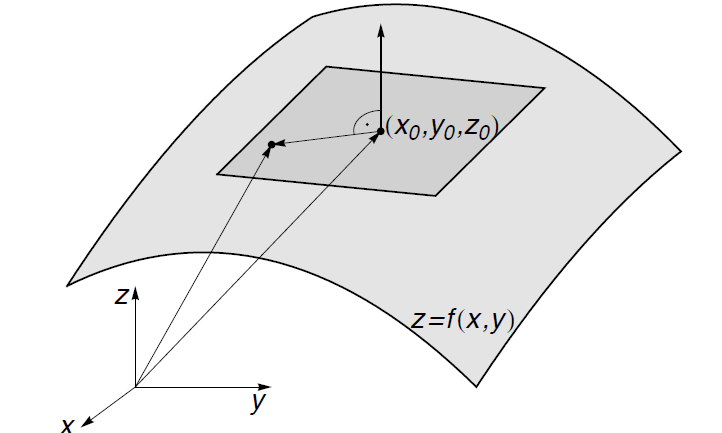
\includegraphics[scale=0.3]{images/plan_tangent2} avec $z_0 = f(x_0,y_0)$
\begin{boite}
conclusion : différentiable $ \iff$ l'existence d'un plan tangent
\end{boite}

\noindent\evid{Fonction continue mais pas différentiable}\\
(voir exemple 4, section 3.2)\\
$f(x,y) = \left\{\begin{array}{ll}
	\frac{x^2y}{x^2+y^2} & (x,y) \neq (0,0)\\
	0 & (x,y) = (0,0)
\end{array}\right.$\\
$f$ est continue sur $\R^2$ (voir la série 3.2)\\
\underline{Méthode A} (différentiable)
\begin{enumerate}[label=\roman*)]
	\item 	$\frac{\delta f}{\delta x}(0,0) = \llimite{h\to 0}{h\neq 0}{\frac{0-0}{h}} = 0\\
			\frac{\delta f}{\delta y}(0,0) = \llimite{h\to 0}{h\neq 0}{\frac{0-0}{h}} = 0$
	\item pour $(x,y) = (0,0)$ on trouve $r(x,y) = \frac{x^2y}{(x^2+y^2)^{\frac{3}{2}}}$ et $\llimite{x\to 0}{x > 0}{r(x,x)} = \llimite{x\to 0}{x>0}{\frac{x^3}{2^{\frac{3}{2}}x^3}} = \frac{1}{2^{\frac{3}{2}}} \neq 0$, donc la fonction n'est pas différentiable.
\end{enumerate}

\section[Fonction diff $\rn \to \Rm$]{Fonctions différentiables de \rn dans \Rm}
\setcounter{equation}{0}
= champs vectoriels sur \rn\\
\underline{Attention :} On ne suivra pas la numérotation du document de référence.

\subsection{Définitions}
Soit $f:D \to \Rm\ , \ \textbf{x}\to f(\textbf{x})\ , \ \textbf{x}=(x_1,...,x_n) \in D$, où $D \subset \rn$ est ouvert.\\
On a $f(\textbf{x}) = f_1(\textbf{x}),\ldots,f_m(\textbf{x}))^T \in \Rm$
\begin{boite}
	\evid{Définition :} (dérivable = partiellement différentiable)\\
	La fonction f est dérivable en $\textbf{x}_0 \in D$, si les dérivées partielles 
	\begin{equation*}
		\frac{\delta f_i}{\delta x_j}(\textbf{x}_\delta) \in \R
	\end{equation*}
	existent pour $i = 1,...,m$ et $j=1,...,n$ (existence des limites
\end{boite}
\begin{boite}
	\evid{Définition :}  (différentiable)\\
	La fonction $f$ est différentiable en $\textbf{x}_0 \in  D \subset \rn$, s'il existe une matrice A (A = {dessin matrice mxn})
	telle que 
	\begin{equation*}
		f(\textbf{x}_0 + \textbf{h}) = f(\textbf{x}_0) + \underbrace{A\overbrace{\textbf{h}}^{\rn}}_{\in \Rm} + r(\textbf{x}_0 + h)||\textbf{h}|| (**)
	\end{equation*}
	avec $\llimite{\textbf{h}\to 0}{\textbf{h}\neq 0}{r(\textbf{x}_0 + \textbf{h})} = 0$
\end{boite}
\begin{boite}
	\evid{Remarque :} (**) $\to A = A_{ij}, i = 1,...,m,\ j=1,...,n\\
	A_{ij} = \frac{\delta f_i}{\delta x_j}(\textbf{x}_0) \in \R$
\end{boite}
\begin{boite}
	\evid{Notation} on écrira $f'(\textbf{x}_0)$ au lieu de $A$ pour la dérivée de $f$ en $\textbf{x}_0$
\end{boite}
\begin{boite}
	remarque : (**) $\iff$
	\begin{equation*}
		\llimite{\textbf{h}\to 0}{\textbf{h} \neq 0}{\underbrace{\frac{f(\textbf{x}_0 + \textbf{h}) - f(\textbf{x}_0) - f'(\textbf{x}_0)\textbf{h}}{||h||}}_{\equiv r(\textbf{x}_0,\textbf{h})}} = \llimite{h\to 0}{h\neq 0}{r(\textbf{x}_0,\textbf{h})} 0
	\end{equation*}
\end{boite}
\begin{boite}
\evid{Terminologie}\\
Le document de référence utilise la notation 
\begin{equation*}
	J_f(\textbf{x}_0) \quad \text{(matrice Jacobienne)}
\end{equation*}
pour la matrice A (si $m > 1$). Mais réservons cette notation pour le cas $n = m$
\end{boite}
\begin{boite}
	\evid{Théorème }Si les fonctions $\frac{\delta f_i}{\delta x_j}$ sont toutes continues sur $D$, alors $f$ est différentiable dans $D$
\end{boite}
$\flat$ même bémol (
\includegraphics[scale=0.1]{images/smiley_rouge}
\includegraphics[scale=0.1]{images/smiley_rouge})
\begin{boite}
	 \evid{Définition} La fonction $f:D \to \Rm\ , \ \textbf{x}\to f(\textbf{x})\ , \ \textbf{x}=(x_1,...,x_n) \in D$, où $D \subset \rn$ est ouvert, est de classe $C^k$ si les fonctions $f_i : D\to \R$ sont de classe $C^k(D)$, pour $i=1,...,m$.
\end{boite}

\subsection{Dérivées de fonctions composées}
\subsubsection{Théorème (dérivée en chaîne)}
\begin{boite}
		\evid{Théorème} Soit 
		\begin{equation*}
			\rn \overset{h}{\longrightarrow} \Rm \overset{g}{\longrightarrow} \R^l\ \text{ avec } f = g\circ h
		\end{equation*}
		$\ulcorner$ Hypothèse $D \equiv D(h) \overset{h}{\longrightarrow} h(D) \subset D(y)$ (la composition est bien définie, et $D \equiv D(h) = D(f) \lrcorner$

	Supposons que $h,g$ sont de classe $C^1$. Soit $\textbf{x}_0 \in D$.\\
	$h'(\textbf{x}_0') = $ une matrice $m\times n$ 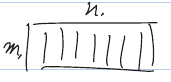
\includegraphics[scale=0.3]{images/mn}\\
	$g'(\underbrace{h(\textbf{x}_0)}_{y_0}) = $ une matrice $l\times m$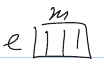
\includegraphics[scale=0.4]{images/lm}\\
	Alors f est de classe $C^1$ et pour $\textbf{x}_0 \in D$ on a 
	\begin{equation*}
		\fcolorbox{red}{white}{$\underbrace{f'(\textbf{x}_0)}_{l\times n} = \underbrace{g'(h(\textbf{x}_0))}_{l\times m} \cdot \underbrace{h'(\textbf{x}_0}_{m\times n})$}
	\end{equation*}
	\begin{center}
		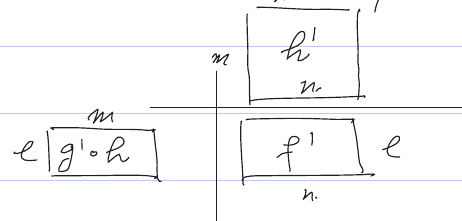
\includegraphics[scale=0.5]{images/multimat}
	\end{center}
\end{boite}
\begin{boite}[0.7]
	\evid{Notation (courte):} Souvent on écrit juste $f' = g' \cdot h'$
\end{boite}

\subsubsection{Exemples (avec démonstration)}
Soit $g: D \to \R,  (x,y) \to g(x,y),\ (x,y) \in D$, où$D$ est ouvert et $h: I \to \R^2,\ t \to h(t) = (h_1(t), h_2(t)),\ t\in I \subset \R$ ouvert, tel que $h(t) \in D$ pour tout $t\in I$\\
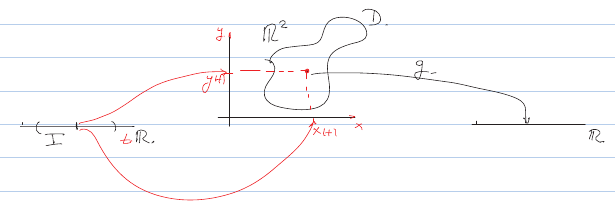
\includegraphics[scale=0.9]{images/compo1}\\
\Big(note : $\big(h_1(t),h_2(t\big)$ s'écrit parfois $\big(x(t), y(t)\big)$\Big)\\
On peut considérer la fonction $f:I\to \R$
\begin{equation*}
	f(t) = (g\circ h)(t) = g(h(t))
\end{equation*}
Supposons que $g$ et$h$ sont de classe $C^1$. Alors on a 
\begin{align*}
	f'(t) = g'(h(t)) \cdot h'(t)\\
	f'(t) = (\frac{\delta g}{\delta x}(h(t)), \frac{\delta g}{\delta y}(h(t))) \cdot \combi{h_1'(t)}{h_2'(t)}
\end{align*}
avec la notation $x(t) = h_2(t),y y(t) = h_2(t)$ :
\begin{align*}
	f'(t) = \(\frac{\delta g}{\delta x}\big(x(t),y(t)\big), \frac{\delta g}{\delta y}\big(x(t),y(t)\big)\) \cdot \combi{x'(t)}{y'(t)}\\
	f'(t) = \underbrace{\frac{\delta g}{\delta x}\big(x(t),y(t)\big) x'(t)}_{\text{dérivée en chaîne pour }x} + \underbrace{\frac{\delta g}{\delta y}\big(x(t),y(t)) y'(t\big)}_{\text{dérivée en chaîne pour }y}
\end{align*}
\begin{boite}
\evid{Notation courte} (avec $f'(t) \equiv \frac{\delta f}{\delta t},\ x'(t) = \frac{\delta x}{\delta t},\ y'(t) = \frac{\delta y}{\delta t}$)\\
$\frac{\delta f}{\delta t} = \frac{\delta g}{\delta x}\frac{\delta x}{\delta t} + \frac{\delta g}{\delta y}\frac{\delta y}{\delta t}$
\end{boite}
\underline{Démonstration de (*)}\\
$\begin{array}{ll}
f'(t) 	& = \limite{s\to 0}\frac{f(t+s) - f(t)}{s}\\
		& = \limite{s\to 0}\frac{g(x(t+s), y(t+s)) - g(x(t), y(t))}{s}\\
		& = \limite{s\to 0}\frac{g(x(t)) + \overbrace{x'(t)s + o(s)}^{\equiv h},}{.} \\
		&= trou \\
		&= \limite{s\to 0}{A 
		\begin{pmatrix}
		\frac{h}{s}\\
		\frac{h}{s}
		\end{pmatrix} + \frac{o(s)}{s})} = A 
		\begin{pmatrix}
		x'(t)\\
		y'(t)
		\end{pmatrix}
\end{array}$
Sous les mêmes hypothèses : $n=1, m=3, l=1. g(x,y,z) \ \ h(t) = (x(t), y(t), z(t))$
\subsubsection{Exemples}
$n=m=2,\ l=1,\ f= g\circ h,\ \R^2 \underset{h}{\longrightarrow} \R^2 \underset{g}{\longrightarrow} \R,\ (u,v) \to (x,y)$\\
$g(x,y)\ , \ h(u,v) = \combi{h_1(u,v)}{h_2(u,v)} \equiv \combi{x(u,v)}{y(u,v)}$\\
$f(u,v) = (g\circ h)(u,v) = g\big(x(u,v),y(u,v)\big)$\\
$f'(u,v) = (g'\circ h)(u,v) \cdot h'(u,v)$\\
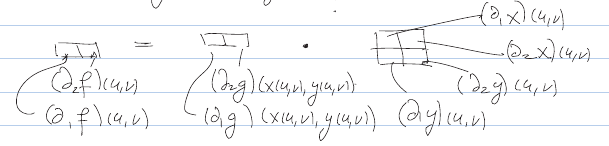
\includegraphics[scale=0.5]{images/compo2}\\
\evid{Notation courte}\\
$\frac{\delta f}{\delta u} = \frac{\delta g}{\delta x} \frac{\delta x}{\delta u} + \frac{\delta g}{\delta y}\frac{\delta y}{\delta u}\\
\frac{\delta f}{\delta v} = \frac{\delta g}{\delta x} \frac{\delta x}{\delta v} + \frac{\delta g}{\delta y}\frac{\delta y}{\delta v}$\\
\evid{Notation complète}\\
$\frac{\delta f}{\delta u}(u,v) = \frac{\delta g}{\delta x}(x(u,v),y/u,v)) \frac{\delta x}{\delta u}(u,v) + \frac{\delta g}{\delta y}(x(u,v),y(u,v)) \frac{\delta y}{\delta u}(u,v)$\\
(avec v pareil)
\subsubsection{Exemples explicites}
\begin{enumerate}
	\item 	$g(x,y) = x^y \ , \ x(t) = \ln(t), y(t) = \sin(t) \to f(t) = g\big(x(t),y(t)\big) = \ln(t)^{\sin(t)} = (g\circ h)(t)$ avec $h(t) = \combi{x(t)}{y(t)}$\\
			La composition est bien définie pour $t>1$\\
			On a\\
			$g'(x,y) = (yx^{y-1}, x^y\ln(x))$\\
			$h'(t) = \combi{\frac{1}{t}}{\cos(t)}$\\
			Donc $f'(t) = (yx^{y-1}, x^y\ln(x)) |_{\substack{x = x(t)\\ y = y(t)}} \cdot \combi{\frac{1}{t}}{\cos(t)}$\\
			ou explicitement \\
			$\begin{array}{ll}
				f'(t) 	&= \sin(t)\ln(t)^{\sin(t)-1} \frac{1}{t} + \ln(t)^{\sin(t)} \ln(\ln(t)) \cos(t)\\
						&=\ln(t)^{\sin(t)}\(\frac{\sin(t)}{t\ln(t)} + \ln(\ln(t)) \cos(t)\)
			\end{array}$
	\item 	$g(x,y) = x^2+y^2 \ , 
			\left\{\begin{array}{ll}
				x=r\cos(\varphi) &\equiv x(r,\varphi)\\
				y=r \sin(\varphi) & \equiv y(r,\varphi)
			\end{array}\right. $\\
			$f(r,\varphi) = g(r\cos(\varphi), r\sin(\varphi) \quad (=r^2)$\\
			$h(r,\varphi) = \combi{x(r\varphi)}{y(r,\varphi)} = \combi{r\cos(\varphi)}{r\sin(\varphi)}$\\
			On s'intéresse à la dérivée de f\\
			$g : \R^2 \to \R$ domaine de \textit{g} est tout $\R^2$\\
			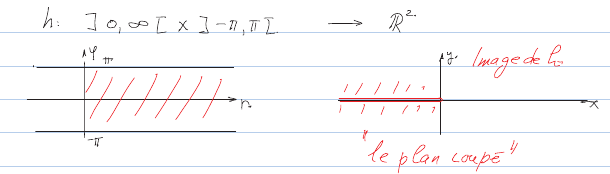
\includegraphics[scale=0.5]{images/fonction_h}\\
			$f = g\circ h\quad ]0,\infty[\ \times\ ]-\pi, \pi[ \to \R$\\
			\uline{Calcul de $f'$} (utiliser que $f(r,\varphi) = r^2$)\\
			$\left.\begin{array}{l}
				\frac{\delta f}{\delta r}(r,\varphi) = 2r\\
				\frac{\delta f}{\delta \varphi}(r,\varphi) = 0
			\end{array}\right\}$ donc $f'(r,\varphi) = (2r,0)$\\
			\uline{Calcul de $f'$ par dérivées en chaîne} (tous les détails)\\
			$g'(x,y) = (2x,2y)\\
			h'(r,\varphi) =
			\begin{pmatrix}
				\cos(\varphi) & -r\sin(\varphi)\\
				\sin(\varphi) & r\cos(\varphi)
			\end{pmatrix}\\
			f'(r,\varphi) = g'(r\cos(\varphi),r\sin(\varphi)) \cdot h'(r,\varphi$\\
			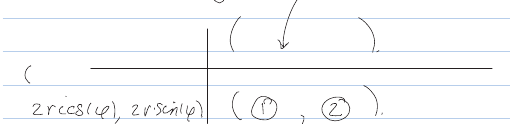
\includegraphics[scale=0.5]{images/repere_matrice_h}\\
			$\circled{1} \frac{\delta f}{\delta r}(r,\varphi) = 2r\cos(\varphi)^2 + 2r\sin(\varphi)^2 = 2r\\
			\circled{2} \frac{\delta f}{\delta \varphi}(r,\varphi) = -2r^2 \cos(\varphi) \sin(\varphi)+ 2r^2\sin(\varphi)\cos(\varphi) = 0$\\
			\uline{Notation courte}\\
			$\frac{\delta f}{\delta r} = \frac{\delta g}{\delta x}\frac{\delta x}{\delta r} + \frac{\delta g}{\delta y}\frac{\delta y}{\delta r} = 2x\cos(\varphi)+2y\sin(\varphi)|_{\text{avec } x=x(r,\varphi),\, y=y(r,y\varphi)} = 2r\cos(\varphi)^2+2r\sin(\varphi)^2 = 2r$\\
			$\frac{\delta f}{\delta \varphi} = \frac{\delta g}{\delta x}\frac{\delta x}{\delta \varphi} + \frac{\delta g}{\delta y}\frac{\delta y}{\delta \varphi} = 2x(-r\sin(\varphi)) + 2y(r\cos(\varphi))|_{\text{avec } x=x(r,\varphi),\, y=y(r,y\varphi)} = 0$
\end{enumerate}
\subsection[$\rn \to \Rm$, Changement de variables]{Fonctions différentiables  de \rn dans \rn, changement de variables}
\begin{boite}
	\evid{Définition} (n=2) Soit $f, \overline{f}, h$\\
	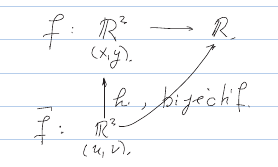
\includegraphics[scale=0.75]{images/fonction_diff} attention, h = G\\
	tels que $\overline{f}(u,v) = f(x,y)$ si $(x,y) = G(u,v)$, alors G est appelé un changement de variable
\end{boite}
\evid{Remarque} $\overline{f}(u,v) = f(G(u,v))\quad f(x,y) = \overline{f}(G^{-1}(u,v))$
\subsubsection{Changement de coordonnées linéaires}
\evid{Exemple} Soit $f: \R^2 \to \R$ (de classe $C^2$) et soit le changement de coordonnées linéaires
\begin{equation*}
u = 3x+y \ , \ v = x-2y
\end{equation*}
On a $\combi{u}{v} = 
\underbrace{\begin{pmatrix}
	3 & 1\\
	1 & 2
\end{pmatrix}}_{A, \det(A) = -7}
\combi{x}{y}$\\
$\combi{x}{y} = A^{-1} \combi{u}{v} \equiv G(u,v) = 
\begin{pmatrix}
	\frac{3}{7} & \frac{1}{7}\\
	\frac{1}{7} & -\frac{3}{7}
\end{pmatrix} \combi{u}{v}$\\
On a donc $\overline{f}(u,v) = (f\circ G)(u,v)  = f(\frac{2}{7}u + \frac{1}{7}v,\ \frac{1}{7}u-\frac{3}{7}v)$
\begin{boite}
	\evid{Définition : Le \textit{Laplacien} de f} Soit $f:\R^2 \to \R \ , \ (x,y) \to f(x,y)$ de classe $C^2$. Si$(x,y) $ sont des coordonnées cartésiennes alors la fonction
	$\begin{array}{lllll}
		g: & \R^2 & \to  & \R\\
		& (x,y) & \to & g(x,y) & = \frac{\delta^2 f}{\delta x^2}(x,y) + \frac{\delta^2 f}{\delta y^2}(x,y)\\
		&&&& = (\frac{\delta^2 f}{\delta x^2} + \frac{\delta^2 f}{\delta y^2}) (x,y)
	\end{array}	$ \\
	est appelée le \textit{Laplacien de f}, et l'application \\
	$\begin{array}{rclll}
	\Delta & C^2 (\R^2) & \to & C^0(\R^2)\\
	& f & \to & g=\Delta f & = \frac{\delta^2 f}{\delta x^2} + \frac{\delta^2 f}{\delta y^2}
	\end{array}$\\
	est appelée le \textit{Laplacien}
\end{boite} 
\uline{Remarque} On écrit simplement $\Delta = \frac{\delta^2 f}{\delta x^2}+ \frac{\delta^2 f}{\delta y^2}$\\
\evid{Exemple (suite)}\\
Soit $\overline{f} = f \circ G \ , \ g=\Delta f \ , \ \overline{g} = g \circ G$. \\
Alors $\begin{array}{rl}
\overline{g}(u,v) &= \big(10 \frac{\delta^2 \overline{f}}{\delta u^2} + 2 \frac{\delta^2 \overline{f}}{\delta u \delta v} + 5\frac{\delta^2 \overline{f}}{\delta v^2}\big)(u,v)\\
& = (\overline{\Delta}\overline{f})(u,v)
\end{array}$

Donc $\overline{\Delta} = 10 \frac{\delta^2 \overline{f}}{\delta u^2} + 2 \frac{\delta^2 \overline{f}}{\delta u \delta v} + 5\frac{\delta^2 \overline{f}}{\delta v^2}$

donc $\overline{g}$ est le Laplacien de $\overline{f}$ avec $\overline{\Delta}$ le Laplacien dans les nouvelles coordonnées.

\evid{Vérification de l'expression par $\overline{\Delta}$}\\
On a $u = 3x + y,y v = x-2y$ et on obtient donc \\
$f(x,y) = (\overline{f} \circ G^{-1})(x,y) = \overline{f}(3x + y, x-2y)$ \\
en notation courte
\begin{center}
	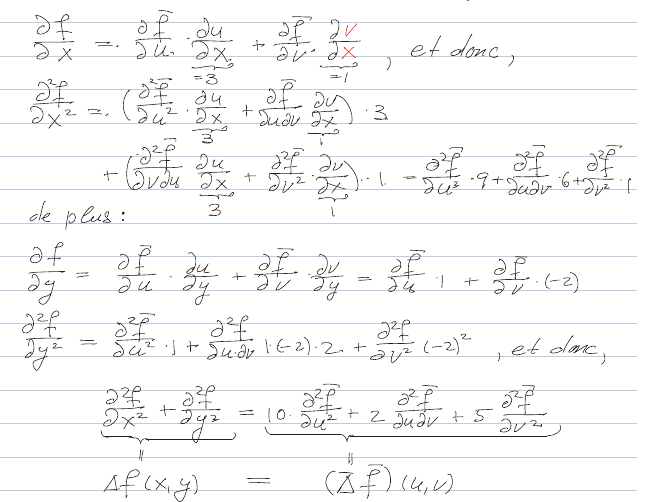
\includegraphics[scale=0.8]{images/sheit}
\end{center}
\uline{Remarque :} (voir algèbre linéaire, changement de vase pour les formes quadratiques)
\includegraphics[scale=0.5]{images/delta}
\subsubsection{Changement de coordonnées non-linéaires}
\evid{Exemple} Soit $f:\R^2 \to \R \ , \ (x,y) \to f(x,y)$ de classe $C^2$. Soit $\overline{f}$ définie par le changement de variables 
\begin{equation*}
	G : ]0,\infty[\ \times\ ]-\pi,\pi[ \to \R^2 \setminus ]-\infty,0[
\end{equation*}
Donc $\overline{f}(r,\varphi) = (f\circ G)(r,\varphi)$. Soit $g = \Delta f$ et $\overline{g} = g\circ G$\\
\begin{boite}
	\uline{Proposition} On a \\
	$\begin{array}{rl}
		\overline{g} (r,\varphi)& = (\overline{\Delta}\overline{f}(r,\varphi)\\
		& = \frac{\delta^2 \overline{f}}{\delta r^2}(r,\varphi) + \frac{1}{r}\frac{\delta \overline{f}}{\delta r}(r,\varphi) + \frac{1}{r^2} \frac{\delta^2 \overline{f}}{\delta \varphi^2}(r,\varphi)
	\end{array}$
\end{boite}
On a $\combi{x}{y} = G(r,\varphi) = \combi{r\cos(\varphi)}{r\sin(\varphi)} \equiv \combi{x(r,\varphi)}{y(r,\varphi)}$\\
et donc 
\begin{boite}
	$G'(r,\varphi) = 
	\begin{pmatrix}
		\cos(\varphi) & -r\sin(\varphi)\\
		\sin(\varphi) & r\cos(\varphi)
	\end{pmatrix} \equiv 
	\begin{pmatrix}
	\frac{\delta x}{\delta r} & \frac{\delta x}{\delta \varphi}\\
	\frac{\delta y}{\delta r} & \frac{\delta y}{\delta \varphi}
	\end{pmatrix}$
\end{boite}
{trou}
\begin{boite}
	\evid{Notation} La dérivée d'une changement de coordonnées $G:\rn \to \rn$ est une matrice $n\times n$. Cette matrice s'appelle aussi la matrice Jacobienne du changement de coordonnées et on écrit souvent $J_G$ au lieu de $G'$ dans ce contexte.
\end{boite}
\uline{Attention} Dans la littérature on trouve la notation $J_F$ au lieu de $F'$ pour la dérivée d'une fonction de $\rn$ dans $\Rm$
\begin{enumerate}[label=\roman*)]
	\item 	Vérification de l'expression pour $\overline{\Delta}$\\
			De $\overline{f}(r,\varphi) = f(r\cos(\varphi),r\sin(\varphi)) = f(x,y)$
			\begin{center}
				\evid{Note : $\delta_1 f = \frac{\delta f}{\delta x},\ \delta_2f  = \frac{\delta f}{\delta y}$}
				\includegraphics[scale=0.7]{images/deriv_delta}
				\includegraphics[scale=0.7]{images/donc_on_trouve_bien}
			\end{center}
	\item 	Comment trouver l'expression pour $\overline{\Delta}$ ? Il faut passer par le changement de variables inverse. Soit 
			\begin{equation*}
				H :) G^{-1}
			\end{equation*}
			\begin{center}
				\includegraphics[scale=0.7]{images/ou_encore}
				\includegraphics[scale=0.7]{images/donc}
				\begin{boite}
					\evid{Théorème} Si G est bijectif, alors $\det(J_G) \neq 0$. Réciproquement, si $\det(J_G) \neq 0$ en un point, alors $G$ est bijectif dans un voisinage de ce point
				\end{boite}
				\includegraphics[scale=0.7]{images/ainsi}
			\end{center}
\end{enumerate}

\evid{Coordonnées sphériques}\\
\includegraphics[scale=1]{images/coord_sph}\\
$\begin{pmatrix}
	x\\
	y\\	
	z
\end{pmatrix} = G(r,\theta,\varphi) =
\begin{pmatrix}
	r\sin(\theta)\cos(\varphi)\\
	r\sin(\theta)\sin(\varphi)\\
	r\cos(\theta)
\end{pmatrix}\\
\begin{array}{ll}
	G 	&: [0,\infty[\ \times\ [0,\pi] \times [0,2\pi] \underset{\text{surjectif}}{\longrightarrow} \R^3\\
 		&:\ ]0,\infty[\ \times\ ]0,\pi[\ \times\ ]0,2\pi[\ \underset{\text{bijectif}}{\longrightarrow} \R^3 \setminus\{(x,0,z) \subset \R^3 : x \geq 0\}
\end{array}\\
J_g(r,\theta,\varphi) = \begin{pmatrix}
{trou}\ matrice\ de\ fou
\end{pmatrix}$
Voir série 7

\subsection{Dérivée d'une intégrale dépendant d'un paramètre}
	\evid{Analyse I}\\
	Soit $f:\rtor$ continue, $a\in\R$. Alors la fonction $G:\rtor$
	\begin{equation*}
		G(t) = \intx{a}{t}{f(x)}
	\end{equation*}
	est de classe $C^1(\R)$ et $\frac{d}{\deriv{t}}G(t) = f(t)$ (Théorème fondamental du calcul intégral)
	
	\evid{Généralisation}\\
	Soit $b: \rtor$ de classe$C^1$. Alors 
	\begin{equation*}
		\frac{d}{\deriv{t}} G(b(t)) = G'(b(t))b'(t) = f(b(t))b'(t)
	\end{equation*}
	Donc si $F(t) ? \intx{a}{b(t)}{f(x)}$ alors $\frac{d}{\deriv{t}}F(t) = f(b(t)) b'(t)$\\
	et si $a:\rtor$ est une fonction de classe $C^1$ et $b\in\R$, alors si
	\begin{equation*}
		F(t) = \intx{a(t)}{b}{f(x)}
	\end{equation*}
	alors
	\begin{equation*}
		F'(t) = \frac{d}{\deriv{t}}\(-\intx{b}{a(t)}{f(x)}\) = -f'(a(t)) a'(t)
	\end{equation*}
	Soit maintenant $F(t) = \intx{a(t)}{b(t)}{f(x)}\quad a,b \in C^1(\R)$, f continue sur \R\\
	{trou}\\
	alors
	\fcolorbox{red}{white}{$F'(t) = f(b(t))b'(t) - f(a(t))a'(t)$}
\begin{boite}
\uline{Proposition} Soit 
\begin{equation*}
F(t) = \intx{a(t)}{b(t)}{f(x,t)}, \quad f\in C^1(\R^2),\ a,b \in C^1(\R)
\end{equation*}
Alors
\begin{equation*}
	F'(t) = f(b(t),t) b'(t) - f(a(t),t)a'(t) + \intx{a(t)}{b(t)}{\frac{\delta f}{\delta t}(x,t)}
	\label{derivee}
\end{equation*}
\end{boite}

\evid{Remarque} Dans le cas particulier où $a(t) = a \in \R,\ b(t) = b\in \R$ sont des fonctions constantes, on a 

\begin{boite}
	\begin{equation*}
	F'(t) = \intx{a}{b}{\frac{\delta f}{\delta t}(x,t)}
	\label{derivee_integrale}
	\end{equation*}
\end{boite}
\evid{Idée de la démonstration de \eqref{derivee_integrale}}
Par définition de la dérivée, on a \\
$\begin{array}{ll}
	F'(t) &= \llimite{h\to 0}{h\neq 0}{\frac{F(t+h) - F(t)}{h}}\\
	& = \llimite{h\to 0}{h\neq 0}{\frac{1}{h}\big(\intx{a}{b}{f(x,t+h)} - \intx{a}{b}{f(x,t)}\big)}\\
	& = \llimite{h\to 0}{h\neq 0}{\intx{a}{b}{\frac{f(x,t+h) - f(x)}{h}}}\\
	&= \intx{a}{b}{\underbrace{\llimite{h\to 0}{h\neq 0}{\frac{f(x,t+h) - f(x)}{h}}}_{= \frac{\delta f}{\delta t} (x,t)}}
\end{array}$
Les deux derniers sont-ils égaux ? Oui, pour $a,b \neq \infty$ et pour $\frac{\delta f}{\delta t}$ une fonction continue, car dans ce cas on a 
\begin{equation*}
	\left|\frac{\delta f}{\delta t}(x,t) - \frac{f(x,t+h) - f(x,t)}{h} \)| < \epsilon
\end{equation*}
pour $t$ donné et $h$ suffisamment petit, \uline{indépendant de $x\in [a,b]$}

\evid{Démonstration de ~\eqref{derivee} avec dérivation en chaine}\\
{trou démonstration}\\
et donc, puisque $F(t) = g(\underbrace{a(t),b(t),t}_{= h(t) = (a(t),b(t),t)^T}) = (g\circ h)(t)$ on a $F'(t) = \frac{\delta g}{\delta a}(a(t),b(t),t)a'(t) +  \frac{\delta g}{\delta b}(a(t),b(t),t)b'(t) +  \frac{\delta g}{\delta t}(a(t),b(t),t)\cdot 1$	

\evid{Exemples}
\begin{enumerate}
	\item 	$F(t) = \intx{0}{\pi}{\frac{\sin(tx)}{x}} \ , \ F'(\frac{1}{4}) = ?$\\
			$F'(t) = \intx{0}{\pi}{\frac{\cos(tx)x}{x}} = \intx{0}{\pi}{\cos(tx)}$\\
			$F(\frac{1}{4}) = \intx{0}{\pi}{\cos(\frac{1}{4}x)} = \left[\sin(\frac{1}{4}x)\)]^\pi_0 = 4\sin(\frac{\pi}{4}) = 2\sqrt{2}$
	
	\item 	$F(t) = \intx{0}{t^2}{\frac{\sin(tx)}{x}} \ , \ F'(\frac{1}{4}) = ?$\\
			$F'(t) = \frac{\sin(t^3}{t^2}(2t) + \intx{0}{t^2}{\cos(tx)}$\\
			$ = 2\frac{\sin(t^3)}{t} + \left[\frac{\sin(tx)}{t}\)]^{x=t^2}_{x=0}$\\
			$ = 2\frac{\sin(t^3)}{t} + \frac{\sin)t^3}{t} = 3\frac{\sin(t^3}{t}$\\
			$F'(\frac{1}{4}) = 12\sin(\frac{1}{64})$
	
	\item 	$F(t) = \intx{0}{1}{\frac{x^t - 1}{\ln(x)}}$\\
			$D(F) = ]-1,\infty[$ (voir Analyse 1)\\
			$\begin{array}{ll}
			F'(t) 	&= \intx{0}{1}{\frac{x^t\ln(x)}{\ln(x)}} = \intx{0}{1}{x^t}\\
					&= \llimite{\epsilon \to 0}{\epsilon > 0}{\intx{\epsilon}{1}{x^t}} = \llimite{\epsilon \to 0}{\epsilon > 0}{\left[\frac{x^{t+1}}{t+1}\)]^{x=1}_{x=\epsilon}} = \frac{1}{t+1}
			\end{array}$
			Donc $F(t) = \ln(t+1) + C$ pour un certain $C$. Puisque $x^0 = 1$, pour tout $x\in ]0,1]$ on a 
			\begin{equation*}
				F(0) = \llimite{\epsilon \to 0}{\epsilon > 0}{\intx{\epsilon}{1}{\underbrace{\frac{x^0 -1}{\ln(x)}}_{= 0}}}
			\end{equation*}
			Mais $F(0) = \ln(0+1) + C = 0+C$ et donc $C=0$\\
			Donc $F(t) = \ln(1+t)$. Ceci donne par exemple
			\begin{equation*}
				\intx{0}{1}{\frac{x-1}{\ln(x)}} = F(1) = \ln(2)
			\end{equation*}
\end{enumerate}

\subsection{Théorème des fonctions implicites}
\includegraphics[scale=0.5]{images/fonctions_implicites}\\
$f_1$ et $f_2$ dont continues sur $[-1,1]$ et dérivables sur $]-1,1[$\\
Comment définir les fonctions $f_1,f_2$ sans isoler $y$ ?
\begin{boite}
	\evid{Théorème des fonctions implicites}\\
	Soit $U \subset \R^2$, ouvert et $F : U \to \R,\ (x,y) \to f(x,y)$ une fonction de classe $C^1$, telle que
	\begin{boite}
	\begin{equation*}
			F(x_0,y_0) = 0,\ \frac{\delta F}{\delta y}(x_0,y_0) \neq 0
	\end{equation*}
	\end{boite}
	pour un $x_0,y_0$. Alors l'équation $F(x,y) = 0$ définit localement (c.-à.-d. par x proche de $x_0$) une fonction $f(x)$ de classe $C^1$ telle que 
	\begin{boite}
	\begin{equation*}
			f(x_0) = y_0 \text{ et } F(x,f(x)) = 0
	\end{equation*}
	\end{boite}
	De plus 
	\fcolorbox{red}{white}{$f'(x) = -\frac{\frac{\delta F}{\delta x} (x,f(x))}{\frac{\delta F}{\delta y}(x,f(x))}$}(*)
\end{boite}
\evid{Démonstration de (*)} On a $F(x,f(x)) = 0$ et donc $\delta_1 F(x,f(x)) + \delta_2 F(x,f(x))f'(x) = 0$ puis on isole $f'(x)$\\
De (*) on trouve en particulier pour $x=x_0$
\begin{boite}[0.6]
\begin{equation*}
		f'(x_0) = -\frac{\frac{\delta F}{\delta x} (x_0,y_0)}{\frac{\delta F}{\delta y}	(x_0,y_0)}\quad (**)
\end{equation*}
\end{boite}
car $f(x_0) = y_0$. On peut donc calculer $f'(x_0)$ sans connaissance explicite de $f$

\evid{Dérivées d'ordre supérieur}\\
De (*) on trouve par $F$ de classe $C^2$\\
$\begin{array}{l}
	f''(x) = -\frac{\frac{\delta^2 F}{\delta x^2}(x,f(x)) + \frac{\delta^2 F}{\delta y \delta x}(x,f(x))f'(x)}{\frac{\delta F}{\delta y}(x,f(x))} + \frac{\frac{\delta F}{\delta x}(x,f(x))}{\(\frac{\delta F}{\delta y}\big(x,f(x)\big)\)^2} \(\frac{\delta^2 F}{\delta x\delta y} \big(x,f(x)\big) + \frac{\delta^2 F}{\delta y^2}\big(x,f(x)\big)f'(x)\)\\
	\text{et donc en } x_0 \text{ on a avec } f(x_0) = y_0\\
	f''(x_0) = \text{pareil, en remplaçant } x\to x_0,\ f(x) \to y_0
\end{array}$\\
avec $f'(x_0)$ donné par (**). On peut donc calculer $f''(x_0)$ (et puis récursivement $f^{(k)}(x_0),\ k=3,4,...$ et donc le développement limité de $f$ en $x_0$) sans avoir une expression explicite pour $f$.
\begin{boite}[0.7]
\evid{Remarque} Si $f'(x_0) = 0$, alors $f''(x_0) = -\frac{\frac{\delta^2 F}{\delta x^2} (x_0,y_0)}{\frac{\delta F}{\delta y}	(x_0,y_0)}$
\end{boite}
\evid{Exemples}
\begin{enumerate}
	\item 	$F(x,y) = x^2+y^2-1\ , \ F(x,y) = 0$ \includegraphics[scale=0.3]{images/exemple_1}\\
			exemple $(x_0,y_0) = (0,1)$. On a \\
			{trou, livre un peu incomplet}\\
			$\frac{d^2}{dx^2}\sqrt{1-x^2}|_{x=0} = \frac{-1}{\sqrt{1-x^2}} + \frac{x^2}{(1-x^2)^{\frac{3}{2}}}|_{x=0} = -1$
	\item 	$F(x,y) = x^3 + xy + y^3 - 3$ sur $\R^2$\\
			$(x_0,y_0) = 1,1) \ , \ F(1,1) = 0 \ , \ \frac{\delta F}{\delta y} = 1 + 3 \cdot 1^2 = 4 \neq 0$\\
			$\to$ il existe une fonction $f(x)$ telle que $F(x,f(x)) = 0$ pour x proche de 1.\\
		On a $f(1) = 1$ et puisque $\frac{\delta F}{\delta x}(x,y) = 3x^2 + y,\ \frac{\delta F}{\delta y}(x,y) = x+3y^2$\\
			on a \\
			$f'(x) = -\frac{3x^2 + f(x)}{x + 3f(x)^2}$
			et en particulier $f'(1) = -\frac{3+1}{1+3\cdot 1^2} = -1$
\end{enumerate}
\begin{boite}
	\evid{Théorème (version $\R^3$)}\\
	Soit $U \subset \R^3$ ouvert, $F_u \to \R,\ (x,y,z) \to F(x,y,z)$ une fonction de classe $C^1$ telle que 
	\begin{center}
		\includegraphics[scale=0.5]{images/version_r3}
	\end{center}
	pour un $(x_0,y_0,z_0) \in U$. Alors l'équation $F(x,y,z) = 0$ définit localement (c'est à dire pour $(x,y)$ proches de $(x_0,y_0)$ une fonction $f(x,y)$ de classe $C^1$ telle que 
	\begin{equation*}
		z_0 = f(x_0,y_0) \text{ et } F(x,y,f(x,y)) = 0
	\end{equation*}
	De plus
	\begin{equation}
		\frac{\delta f}{\delta x} (x,y) = - \frac{\frac{\delta F}{\delta x}(x,y,f(x,y))}{\frac{\delta F}{\delta z}(x,y,f(x,y))}
	\end{equation}
	\begin{equation}
		\frac{\delta f}{\delta y} (x,y) = - \frac{\frac{\delta F}{\delta y}(x,y,f(x,y))}{\frac{\delta F}{\delta z}(x,y,f(x,y))}
	\end{equation}
\end{boite}
\evid{Explication de (14,15)}\\
De $F(x,y,f(x,y)) = 0$ on trouve\\
$\frac{\delta F}{\delta x}(x,y,f(x,y)) + 0 + \frac{\delta F}{\delta z}(x,y,f(x,y))\frac{\delta f}{\delta x}(x,y,f(x,y)) = 0 \to 14$\\
$0 + \frac{\delta F}{\delta y}(x,y,f(x,y)) + \frac{\delta F}{\delta z}(x,y,f(x,y))\frac{\delta f}{\delta y}(x,y) = 0$

\subsection{Équation du plan tangent bis}
(voir aussi le chapitre 3.4)
\subsubsection{Représentation de surfaces}
Soit $F(x,y,z)$ de classe $C^1$ dans $U\subset \R^3,\ U$ ouvert, tel que 
\begin{equation*}
	F(x_0,y_0,z_0) =0 \text{ et }\frac{\delta F}{\delta z}(x_0,y_0,z_0) \neq 0
\end{equation*}
pour un $(x_0,y_0,z_0) \in U$. Par le théorème des fonctions implicites, il existe donc une fonction $f(x,y)$ de classe $C^1$, définie dans un voisinage de $(x_0,y_0)$ telle que $f(x_0,y_0) = z_0$ et 
\begin{equation*}
	F\big(x,y,f(x,y)\big) = 0
\end{equation*}
Proche de $(x_0,y_0,z_0)$ l'ensemble des points où $F(x,y,z) = 0$ (l'ensemble de niveau 0 de F) est donc une surface et cette surface est le graphe de la fonction $f$.

On a donc deux manières de représenter une surface dans un voisinage d'un point $(x_0,y_0,z_0)$ :
\begin{enumerate}
	\item 	$F(x,y,z) = 0 \quad$ si $F(x_0,y_0,z_0) = 0, \frac{\delta F}{\delta z}(x_0,y_0,z_0) \neq 0$
	\item 	$z = f(x,y) \quad$ si $z_0 = f(x_0,y_0)$
\end{enumerate}
$1\to 2$ par le théorème des fonctions implicites et $2\to 1$ car donné $f(x,y)$ avec $z_0 = f(x_0,y_0)$ on peut toujours prendre $F(x,y,z) = t-f(x,y)$

\subsubsection{L'équation du plan tangent}
Donnée $f$ l'équation du plan tangent en $(x_0,y_0,z_0)$ est 
\begin{equation}
	z = f(x_0,y_0) + \frac{\delta f}{\delta x}(x_0,y_0)(x-x_0) + \frac{\delta f}{\delta y}(x_0,y_0)(y-y_0) \label{plan_tangent}
\end{equation}
\begin{center}
	\includegraphics[scale=0.7]{images/plan_tangent}
\end{center}
\eqref{plan_tangent} $\iff z - z_0 - \frac{\delta f}{\delta x}(x_0,y_0)(x-x_0) - \frac{\delta f}{\delta y}(x_0,y_0)(y-y_0) = 0$\\
\eqref{plan_tangent} $\iff \Big(\underbrace{-\frac{\delta f}{\delta x}(x_0,y_0)}_{= \frac{\frac{\delta F}{\delta x}(x_0,y_0,z_0)}{\frac{\delta F}{\delta z}(x_0,y_0,z_0)}}, \underbrace{-\frac{\delta f}{\delta y}(x_0,y_0)}_{=\frac{\frac{\delta F}{\delta y}(x_0,y_0,z_0)}{\frac{\delta F}{\delta z}(x_0,y_0,z_0)}}, 1\Big)^T \cdot \begin{pmatrix}
x-x_0\\
y-y_0\\
z-z_0
\end{pmatrix} = 0$\\
en multipliant avec $\frac{\delta F}{\delta z}(x_0,y_0,z_0) \neq 0$ on obtient
\begin{equation*}
	\(\underbrace{\frac{\delta F}{\delta x}(x_0,y_0,z_0), \frac{\delta F}{\delta y}(x_0,y_0,z_0), \frac{\delta F}{\delta z}(x_0,y_0,z_0)}_{= \nabla F(x_0,y_0,z_0)}\)\cdot \begin{pmatrix}
x-x_0\\
y-y_0\\
z-z_0
\end{pmatrix} = 0
\end{equation*}
\begin{boite}
\uline{Conclusion :} \\
($\nabla F)(x_0,y_0,z_0)$ est orthogonal au plan tangent en $(x_0,y_0,z_0)$.
\end{boite}

\evid{Exemple} \\
$F(x,y,z) = x^2 + y^2 + z^2 -1\ ; \ F(x,y,z) = 0$ : surface de la sphère de rayon 1\\
Soit $x_0,y_0$ tel que $x_0^2 + y_0^2 < 1$ et $z_0 = \sqrt{1-x_0^2-y_0^2}$. On a $F(x_0,y_0,z_0) = 0$ et $\frac{\delta F}{\delta z}(x_0,y_0,z_0) = 2z_0 \neq 0$\\
De plus, $\frac{\delta F}{\delta x}(x_0,y_0,z_0) = 2x_0\ , \ \frac{\delta F}{\delta y}(x_0,y_0,z_0) = 2y_0$\\
Plan tangent : $(2x_0,2y_0,2z_0)^T \cdot \begin{pmatrix}
x-x_0\\
y-y_0\\
z-z_0
\end{pmatrix} = 0$


\subsection{La dérivée directionnelle}
\subsubsection{Définitions (n=2)}
\begin{boite}
	\evid{Définition} Soit $f:D\to \R(x,y) \to f(x,y)$ où$ D\subset \R^2$ est ouvert. Soit $(x_0,y_0) \in D$ et $\textbf{e} = (e_1,e_2) \in \R^2$ un vecteur unité. Le nombre
	\begin{equation*}
		\frac{\delta f}{\delta \textbf{e}^+}(x_0,y_0) = \llimite{t\to 0}{t> 0}{\frac{f(x_0+te_1,y_0+te_2) - f(x_0,y_0)}{t}}
	\end{equation*}
	est appelée la  \uline{dérivée directionnelle unilatérale} (ou dérivée directionnelle au sens de Dini) de $f$ en $(x_0,y_0)$ suivant le vecteur \textbf{e} et le nombre
	\begin{equation*}
		\frac{\delta f}{\delta \textbf{e}}(x_0,y_0) = \llimite{t\to 0}{t\neq 0}{\frac{f(x_0+te_1,y_0+te_2) - f(x_0,y_0)}{t}}
	\end{equation*}
	est appelée la dérivée directionnelle de $f$ en $(x_0,y_0)$ suivant le vecteur \textbf{e}
\end{boite}
\evid{Remarque :} 
\begin{itemize}
	\item 	Si $\textbf{e}	= (1,0)$ on a $\frac{\delta f}{\delta \textbf{e}}(x_0,y_0) = \frac{\delta f}{\delta x}(x_0,y_0)$
	\item 	Si $\textbf{e}	= (0,1)$ on a $\frac{\delta f}{\delta \textbf{e}}(x_0,y_0) = \frac{\delta f}{\delta y}(x_0,y_0)$
\end{itemize}
\evid{Remarque :}
\begin{itemize}
	\item 	Si $\frac{\delta f}{\textbf{e}}(x_0,y_0)$ existe, alors $\frac{\delta f}{\delta \textbf{e}^+}(x_0,y_0)$ existe et $\frac{\delta f}{\delta \textbf{e}^+}(x_0,y_0) = \frac{\delta f}{\textbf{e}}(x_0,y_0)$
\end{itemize}
\begin{boite}
	\evid{Proposition} Soit $g(t) = f(x_0 + te_1,y_0 + te_2)$. Alors 
	\begin{align*}
		g'(0) =  \frac{\delta f}{\delta \textbf{e}}(x_0,y_0) \text{ et}\\
		\text{(la dérivée à droite de g en 0)}\to g'(0+) =  \frac{\delta f}{\delta \textbf{e}^+}(x_0,y_0)
	\end{align*}
\end{boite}
\uline{Démonstration}\\
$g'(0) = \llimite{t\to 0}{t\neq 0}{\frac{g(t)-g(0)}{t}} = \llimite{t\to 0}{t\neq 0}{\frac{f(x_0+te_1,y_0+te_2) - f(x_0,y_0)}{t}} = \frac{\delta f}{\delta \textbf{e}}(x_0,y_0)$\\
$g'(0+) = \llimite{t\to 0}{t > 0}{\ldots} = \frac{\delta f}{\delta \textbf{e}^+}(x_0,y_0)$\\
\evid{Remarque} C'est une manière de calculer la dérivée directionnelle (unilatérale)\\
\evid{Remarque} Attention : $f$ n'est pas forcément différentiable en $(x_0,y_0)$ (voir plus loin)
\begin{center}
	\includegraphics[scale=0.5]{images/plan_differentiable}
\end{center}
\evid{Exemple} Soit $f(x,y) = 1-\sqrt{x^2-y^2}$ pour $(x,y) \in D$ où $D = D(0,1)$ {trou cercle unité, pas dans le cours}
\begin{enumerate}
	\item 	Par définition : $\frac{\delta f}{\delta \textbf{e}}(0,0) =\llimite{t\to 0}{t\neq 0}{\frac{f(t\cos(\varphi),t\sin(\varphi) - f(0,0)}{t}} = \llimite{t\to 0}{t\neq 0}{\frac{(1-|t|) -1}{t}} = \llimite{t\to 0}{t\neq 0}{\frac{-|t|}{t}}$ n'existe pas\\
			$\frac{\delta f}{\delta \textbf{e}^+}(0,0) = \llimite{t\to 0}{t>0}{\ldots} = \llimite{t\to 0}{t>0}{\frac{-|t|}{t}} = \llimite{t\to 0}{t>0}{-1} = -1$
			{trou graph cône/chapeau}
			
	\item 	avec la fonction $g : \\ g(t) = f(0+t\cos(\varphi), o + t\sin(\varphi)) = 1-|t|$\\
			$g'(0+) = -1 = \frac{\delta f}{\delta \textbf{e}^+}(0,0)$
\end{enumerate}
\includegraphics[scale=0.5]{images/plan_exemple_2}\\
ii) Par la définition :\\
$\frac{\delta f}{\delta \textbf{e}}(0,0)$\\ \includegraphics[scale=0.5]{images/suite_exemple}\\
\includegraphics[scale=0.5]{images/dessins_exemple}\\
\evid{Remarque :} On a nécessairement que 
\begin{equation*}
	\left.\frac{\delta f}{\delta \textbf{e}}(0,0)\right|_{\varphi + \pi} = \left.\frac{\delta f}{\delta \textbf{e}}(0,0)\right|_{\varphi}
\end{equation*}
\begin{boite}
	\evid{Résumé :} $f$ est continue en $(0,0)$, dérivable = partiellement différentiable en (0,0), la dérivée directionnelle existe en (0,0) pour tout vecteur unité \textbf{e}, mais la fonction n'est pas différentiable en (0,0) (donc il n'existe pas de plan tangent en (0,0))
\end{boite}

\subsubsection{Définition pour n général}
\begin{boite}
	\evid{Définition} Soit $f:D\to \R, \textbf{x} \to f(\textbf{x}), \textbf{x} = (x_1,...,x_n) \in D$, où $D \subset \R^n$ est ouvert. Soit $\textbf{e} = (e_1,...,e_n)$ un vecteur unité de $\R^n$ et $\textbf{x}_0 \in D$. Le nombre 
	\begin{equation*}
		\frac{\delta f}{\delta \textbf{e}^+}(\textbf{x}_0) = \llimite{t\to 0}{t>0}{\frac{f(\textbf{x}_0 + t\textbf{e}) - f(\textbf{x}_0)}{t}}
	\end{equation*}
	est appelée \uline{la dérivée directionnelle unilatérale ou dérivée directionnelle au sens de Dini} de $f$ en $\textbf{x}_0$ suivant le vecteur \textbf{e}, et le nombre 
	\begin{equation*}
	\frac{\delta f}{\delta \textbf{e}}(\textbf{x}_0) = \llimite{t\to 0}{t\neq0}{\frac{f(\textbf{x}_0 + t\textbf{e}) - f(\textbf{x}_0)}{t}}
	\end{equation*}
	est appelé la dérivée directionnelle de $f$ en $\textbf{x}_0$ suivant le vecteur \textbf{e}
\end{boite}
\evid{Remarque} Pour $n=1$ la dérivée directionnelle unilatérale pour \textbf{e} = (1) est égale à la dérivée à droite et pour \textbf{e} = (-1) est égale à moins la dérivée à gauche\\
\evid{Remarque} Pour $\textbf{e} = (0,...,0,\underbrace{1}_{\mathclap{\text{position i}}},0,...,0)$ on a 
\begin{equation*}
	\frac{\delta f}{\delta \textbf{e}}(\textbf{x}_0) = \frac{\delta f}{\delta x_i}(\textbf{x}_0)
\end{equation*}

\subsubsection{Le cas où f est différentiable (n=2)}
Soit $f:D\to \R,\ D\subset \R^2$ ouvert, $(x,y) \to f(x,y)$ et $f$ différentiable en $(x_0,y_0)$ et soit $\textbf{e} = (e_1,e_2)$\\
Soit $g(t) = f(x_0 + e_1t,y_0+e_2t) = f(\begin{pmatrix}
x_0+ e_1t\\
y_0+e_2t
\end{pmatrix}) = f(h(t)) = (f\circ h)(t)$\\
Puisque $f$ est différentiable on a (dérivée en chaîne)\\
$\frac{\delta f}{\delta \textbf{e}}(x_0,y_0) = g'(0) = f'(h(0)) h'(0) = f0(x_0,y_0) h'(0) = \nabla f (x_0,y_0) \cdot \textbf{e}$
\begin{boite}
	\evid{Définition (bis)} (cas ou f est différentiable)\\
	Le nombre $\frac{\delta f}{\delta \textbf{e}}(x_0,y_0) := \nabla f(x_0,y_0) \cdot e$ (produit scalaire) est appelé la dérivée directionnelle de f en $(x_0,y_0)$
\end{boite}
\subsection*{Résumé (dérivée directionnelle)}
\begin{enumerate}
	\item 	Par définition : $\frac{\delta f}{\delta \textbf{e}}(x_0,y_0) = \llimite{t\to 0}{t\neq 0}{\frac{f(x_0+te_1,y_0+te_2) - f(x_0,y_0)}{t}}$
	\item 	En termes de la fonction $g(t) = f(x_0+te_1,y_0+te_2)$ \\
			\begin{equation*}
			\frac{\delta f}{\delta \textbf{e}}(x_0,y_0) = g'(0)
			\end{equation*}
	\item 	\uline{Si f est différentiable} en $(x_0,y_0)$ :
			\begin{equation*}
				\frac{\delta f}{\delta \textbf{e}}(x_0,y_0) = \nabla f(x_0,y_0 \cdot e \equiv \frac{\delta f}{\delta x}(x_0,y_0) e_1 + \frac{\delta f}{\delta y})(x_0,y_0) e_2
			\end{equation*}
\end{enumerate}
\evid{Remarques, cas $f$ différentiable} $(n=2)$
\begin{enumerate}
	\item 	$\frac{\delta f}{\delta \textbf{e}}(x_0,y_0)$ est maximale si \textbf{e} pointe dans le sens de $\nabla f(x_0,y_0)$, c'est à dire pour 
			\begin{equation*}
				\textbf{e} = \frac{\nabla f(x_0,y_0)}{||\nabla f(x_0,y_0)||} \quad \text{on suppose que } \nabla f(x_0,y_0) \neq 0
			\end{equation*}
			Pour ce vecteur on a avec iii)
			\begin{equation*}
				\frac{\delta f}{\delta \textbf{e}}(x_0,y_0) = \nabla f(x_0,y_0) \cdot \frac{\nabla f(x_0,y_0)}{||\nabla f(x_0,y_0)} = \frac{||\nabla f(x_0,y_0)||^2}{||\nabla f(x_0,y_0)||} = ||\nabla f(x_0,y_0)||
			\end{equation*}
	\item 	Le gradient est orthogonal aux lignes de niveaux, c'est à dire aux courbes dans le domaine de définition où f est constant.
			{trou images mars 2x}{trou image empiler carton altitude}\\
\end{enumerate}

\evid{Lien avec le théorème des fonctions implicites}\\
{trou graph 4 courbes c1,c2,c3,c4 (a modifier sur gimp)}\\
\evid{Démonstration de ii)}\\
$f$ différentiable veut dire $f(x,y) = f(x_0,y_0) + \frac{\delta f}{\delta y}(x_0,y_0)(x-x_0) + \frac{\delta f}{\delta y}(x_0,y_0)(y-y_0) +$ \enquote{petit}\\
avec \enquote{petit} = $r(x,y) d$ et $d = \sqrt{(x-x_0)^2 + (y-y_0)^2}$ et $\llimite{x\to x_o}{y\to y_0}{r(x,y)} = 0$\\
Sur la courbe, on a $f(x,y) = c = f(x_0,y_0)$. La somme des deux dérivées doit être égale à 0 car \enquote{petit} est plus petit par $(x,y)$ proche de $(x_0,y_0)$ (*). Le seul moyen pour que ça marche, est que cette somme soit 0.\\
Pour $(x,y)$ proche de $(x_0,y_0)$ on a donc :
\begin{equation*}
	(*) \iff \text{\fcolorbox{red}{white}{$\underbrace{\nabla f(x_0,y_0)}_{\equiv \nabla F(x_0,y_0)} \cdot\combi{x-x_0}{y-y_0} = 0$}}
\end{equation*}
Si on isole $y$ dans (*) : 
$\begin{array}{ll}
y &= y_0 - \underbrace{\frac{\frac{\delta f}{\delta x} (x_0,y_0)}{\frac{\delta f}{\delta y}(x_0,y_0)}} (x-x_0)\\
&  = -\frac{\frac{\delta F}{\delta x} (x_0,y_0)}{\frac{\delta F}{\delta y}(x_0,y_0)} = g'(x_0) \text{ (par le théo des fonctions implicites)}
\end{array}$\\
$y = y_0 + g'(x_0)(x-x_0)$ où $F(x,g(x)) = 0, g(x_0) = y_0$
\subsubsection{Le cas où f est différentiable (n arbitraire)}
\begin{boite}
	\evid{Définition (bis)} (cas n différentiable)\\
	Soit $f : D \to \R \ , \ \textbf{x} \to f(\textbf{x}) \ , \ \textbf{x} = (x_1,...,x_n) \in D$ où $D$ ouvert, $D \subset \R^n,\ f$ différentiable en $x_0 \in D$ et $\textbf{e} = (e_1,...,e_n)^T \in \R^n$ un vecteur unitaire. Alors le nombre
	\begin{equation*}
		\frac{\delta f}{\delta \textbf{e}}(x_0) := \nabla f(\textbf{x}_0) \cdot \textbf{e} = \somme{i=1}{n}{\frac{\delta f}{\delta x_i}}(\textbf{x}_0) e_i
	\end{equation*}
	est appelé la dérivée directionnelle de $f$ en $\textbf{x}_0$ suivant le vecteur \textbf{e}
\end{boite}
\evid{Remarque :} Cette définition est équivalente à la définition avec la limite, mais non suppose f différentiable.\\
\evid{Exemples} 
\begin{enumerate}
	\item 	$f(x,y) = e^{xy}${trou}
			\begin{enumerate}
				\item {trou}
				\item 	$g(t) = f(1+\frac{1}{\sqrt{2}} t, 0+\frac{1}{\sqrt{2}} t) = e^{1+\frac{1}{\sqrt{2}} t)(0+\frac{1}{\sqrt{2}}t} = e^{\frac{1}{\sqrt{2}}t + \frac{1}{\sqrt{2}}t^2}$\\
				$\frac{\delta f}{\delta \textbf{e}}(1,0) = g'(0) = \frac{1}{\sqrt{2}}$
			\end{enumerate}
	\item	\begin{enumerate}
				\item 	{trou livre}
				\item 	$g(t) = e^{1+ \frac{1}{\sqrt{3}} t)( 1 + \frac{1}{\sqrt{3}} t)( 0 + \frac{1}{\sqrt{3}} t)} = ...\\
						g'(0) = \frac{1}{\sqrt{3}}$\\
						Le mieux est d'utiliser le développement limité pour calculer $g'(0)$ :
						\begin{equation*}
							g(t) = e^{\frac{1}{\sqrt{3}} t + o(t)} = 1 + \frac{1}{\sqrt{3}}t + o(t)
						\end{equation*}
			\end{enumerate}
\end{enumerate}
\subsection{Approximation de Taylor, développement limité}
\subsubsection{Développement limité d'ordre 1 et et 2}
Soit $f: D \to \R, (x,y) \to f(x,y),$ où $D \subset \R$ est ouvert, $f$ de classe $C^1$ et soit $(x_0,y_0) \in D$. Alors $f$ possède un développement limité d'ordre 1 dans un voisinage de $(x_0,y_0)$. 
\begin{equation*}
f(x,y) = f(x_0,y_0) + \frac{\delta f}{\delta x}(x_0,y_0)(x-x_0) + \frac{\delta f}{\delta y}(x_0,y_0)(y-y_0) + \underbrace{r(x,y) d}_{o(d)} \textcolor{red}{= p_1(x,y)}
\end{equation*}
où $d = \sqrt{(x-x_0)^2 + (y-y_0)^2}$ et $\llimite{x\to x_0}{y\to y_0}{r(x,y)} = 0$\\
Le polynôme linéaire $p_1(x,y)$ est appelé le polynôme de Taylor d'ordre 1 (de f en $(x_0,y_0)$. Ce polynôme approxime f linéairement dans un voisinage de $(x_0,y_0)$.

Si $f$ est de classe $C^2(D)$, alors $f$ possède un développement limité d'ordre deux dans $(x_0,y_0)$\\
$\begin{array}{ll}
	f(x,y) &= f(x_0,y_0) + \frac{\delta f}{\delta x}(x_0,y_0)(x-x_0) + \frac{\delta f}{\delta y}(x_0,y_0)(y-y_0)\\
	& + \frac{1}{2}\frac{\delta^2 f}{\delta x^2}(x_0,y_0)(x-x_0)^2\\
	&+ \frac{1}{2}\frac{\delta^2 f}{\delta y^2}(x_0,y_0)(y-y_0)^2\\
	&+ \underbrace{\frac{1}{2}\cdot 2 \cdot \frac{\delta^2 f}{\delta x\delta y}(x_0,y_0)(x-x_0)(y-y_0)}_{\textcolor{red}{= p_2(x,y)}}\\
	& = \underbrace{f(x_0,y_0) + \nabla f(x_0,y_0) \cdot\combi{x-x_0}{y-y_0} + \frac{1}{2} \combi{x-x_0}{y-y_0} \cdot Hess(f)(x_0,y_0)\combi{x-x_0}{y-y_0}}_{\textcolor{red}{= p_2(x,y)}} + o(d^2)
\end{array}$
où $Hess(f) = \begin{pmatrix}
			\frac{\delta^2 f}{\delta x_1^2 }(x_0,y_0) & \frac{\delta^2 f}{\delta x_1, \delta x_n}(x_0,y_0)\\
			\frac{\delta^2 f}{\delta x_n\delta x_1}(x_0,y_0) & \frac{\delta^2 f}{\delta x_n^2} (x_0,y_0)
	\end{pmatrix}$\\
Le polynôme $p_2(x,y)$ est le polynôme de Taylor d'ordre deux (de f en $(x_0,y_0)$). Il approxime la fonction f d'une manière quadratique dans un voisinage de $(x_0,y_0)$.\\
\evid{Exemple} $f(x,y) = \sin(2x + y) + 3\cos(x+y) \ , \ (x_0,y_0) = (0,0)$.\\
$f(x_0,y_0) = 3,\ \frac{\delta f}{\delta x}(x_0,y_0) = 2 \ , \ \frac{\delta f}{\delta y}(x_0,y_0) = 1, \frac{\delta^2 f}{\delta x^2}(x_0,y_0) = -3, \frac{\delta^2 f}{\delta x \delta y}(x_0,y_0) = -3, \ \frac{\delta^2 f\delta y^2}{(x_0,y_0)} = -3$\\
$p_2(x,y) = 3 + 2x + y - \frac{3}{2}x^2 - 3xy - \frac{3}{2}y^2$
\begin{center}
	\evid{Méthode de calcul univariée (voir la série 9)}
\end{center}
Puisque $2x + y|_{(0,0)} = 0$ et $x+y|_{(0.0)} = 0$ on peut calculer le polynôme $p_2$ par composition des développements limités (DL) de $\sin(z)$ et $\cos(z)$ en $z = z_0 = 0$ avec $2x + y$ et $x+y$. On a 
\begin{align*}
	\sin(z) = z + o(z^2)\\
	\cos(z) = 1 - \frac{1}{2}z^2 + o(z^2)
\end{align*}
et donc \\
$\begin{array}{ll}
	f(x,y) 	&= (2x + y) + 3(1 - \frac{1}{2}(x+y)^2) + o((2x+y)^2) + o((x+y)^2)\\
			&= \underbrace{3 + 3x + y -\frac{3}{2}x^2 - 3xy - \frac{3}{2}y^2}_{=p_2(x,y)} + o(d^2)
\end{array}$\\
\evid{Remarque (rappel!) concernant le reste $o(d^2)$}\\
On a $\(|x| - |y|\)^2 = x^2 + y^2 - 2|x||y| \geq 0 \to 2|x||y| \leq x^2 + y^2 = d^2$\\
donc \\
$(x+y)^2 \leq x^2 + y^2 + 2|x||y| \leq 2d^2\\
(2x + y)^2 \leq 4x^2 + y^2 + 4|x||y| \leq 4x^2 + 4y^2 + 4|x||y| \leq 6d^2$
\subsubsection{Le développement limité d'ordre N}

\evid{Rappel :} Soit $f : I\to\R, x\to f(x), x\in I \subset \R$, I ouvert. Soit $f$ de classe $C^N$ dans un voisinage de $x_0 \in I$. Alors 
\begin{equation*}
	f(\underbrace{x}_{x_0 + h}) = f(x_0) + f'(x_0)(\underbrace{x-x_0}_h) + ... + \frac{1}{N!}f^{(N)}(x_0)(\underbrace{x-x_0}_h)^N + o(|\underbrace{x-x_0}_h|^N)
\end{equation*}
ou encore
\begin{equation*}
	f(x_0 + h) = \somme{N}{n=0} \frac{1}{n!} f^{(n)}(x_0) h^n + o(|h|^N)
\end{equation*}
ou encore avec $\frac{d}{dx} : c^k(I) \to C^{k-1}(I),\ f \to \frac{df}{dx} = f'$ avec $\frac{d}{dx}$ une application linéaire.
\begin{align*}
f(x_0 + h) = \somme{N}{k=0} \frac{1}{k!}\(\(h\frac{d}{dx}\)^k f\) (x_0) + o(|h|^N)\\
k = 0 : \(h\frac{d}{dx}\)\text{petit trou}
\end{align*}
\begin{boite}
	\evid{Théorème} Soit la fonction $f: D\to \R,\ \textbf{x}\to f(\textbf{x}),\ D\subset \R^n$ ouvert, $f$ de classe $C^N(D),\ \textbf{x}_0 \in D$. Alors $f$ possède un développement limité d'ordre $N$ dans un voisinage de $\textbf{x}:0$ :
	\begin{equation*}
		f(\textbf{x}_0 + \textbf{h}) = \somme{N}{k=0}\frac{1}{k!}\(\(\textbf{x} \cdot \nabla\)^k f\)(\textbf{x}_0) + o(d^N)
	\end{equation*}
	où $d = ||h||$
\end{boite}
Cas n=2 : développement limité de $f(x,y)$ en $(x_0,y_0)$ :
\begin{equation*}
	f(x_0 + h, y_0 + h) = \somme{N}{l=0} \frac{1}{l!}\(\(h \frac{\delta }{\delta x} + k\frac{\delta}{\delta y}\)^l f\) (x_0,y_0) + o(d^N)
\end{equation*}
\uline{Formule binomiale :}\\
$a+b9^l = \somme{l}{m=0}$ trou\\
\uline{Pour $N = 3$ :}\\
$\begin{array}{ll}
	(x_0, + h, y_0 + h) &= f(x_0,y_0) + h\frac{\delta f}{\delta x} + k\frac{\delta f}{\delta y}(x_0,y_0)\\
		& + \frac{1}{2!}\(\(h \frac{\delta }{\delta x} + k\frac{\delta }{\delta y}\)^2 f\)(x_0,y_0)\\
		& + \underbrace{\frac{1}{3!}\(\(h \frac{\delta }{\delta x} + k\frac{\delta }{\delta y}\)^3 f\)(x_0,y_0)} + o(d^3)\\
		&= p_3(x,y) \text{ le polynôme de Taylor d'ordre 3}\\
\end{array}\\
\begin{array}{ll}
= f(x_0,y_0)& + h\frac{\delta f}{\delta x}(x_0,y_0) + k\frac{\delta f}{\delta y} \\
&+ \frac{1}{2!}h^2\frac{\delta^2 f}{\delta x^2}(x_0,y_0) + \frac{1}{2}k^2 \frac{\delta^2 f}{\delta y^2}(x_0,y_0) + hk \frac{\delta^2f}{\delta x \delta y}(x_0,y_0) \\ 
&+ \frac{1}{3!} h^2 \frac{\delta^3 f}{\delta x^2}(x_0,y_0) + \frac{1}{2}h^2 k \frac{\delta^3 f}{\delta x^2 \delta y}(x_0,y_0) + \frac{1}{2}hk^2 \frac{\delta^3 f}{\delta x\delta y^2}(x_0,y_0) + \frac{1}{3!}k^3 \frac{\delta^3 f}{\delta y^3}(x_0,y_0) + o(d^3)
\end{array}$
$\frac{1}{2}$ car $\combi{3}{2}\frac{1}{3!}$

\section{Extremums locaus et absolus d'une fonction de $n$ variables}
\setcounter{equation}{0}
\subsection{Définitions}
\begin{boite}
	\evid{Définition :} Soit la fonction $f : D \to \R,\ \textbf{x}\to f(\textbf{x}),\ D\subset \R^n$ ouvert, $\textbf{x}_0 \in D$. On dit que f admet en $\textbf{x}_0$ :
	\begin{enumerate}
		\item Un $\overline{\text{maximum}}$ \textit{local} (ou relatif) si et seulement si $f(\textbf{x}) \leq f(\textbf{x}_0)$ pour tout \textbf{x} dans un voisinage de $\textbf{x}_0$.
		\item Un \underline{minimum} \textit{local} (ou relatif) si et seulement si $f(\textbf{x}) \geq f(\textbf{x}_0)$ pour tout \textbf{x} dans un voisinage de $\textbf{x}_0$.
		\item Un $\overline{\text{maximum}}$ \textbf{absolu} (ou global) si et seulement si $f(\textbf{x}) \leq f(\textbf{x}_0)$ pour tout \textbf{x} dans $D$
		\item Un \underline{minimum} \textbf{absolu} (ou global) si et seulement si $f(\textbf{x}) \leq f(\textbf{x}_0)$ pour tout \textbf{x} dans $D$
		\item un point stationnaire (ou point critique) si et seulement si $f$ est différentiable en $\textbf{x}_0$ et $\nabla f(\textbf{x}_0) = 0\ (\in \R^n)$
		\item Un point-selle ssi $\textbf{x}_0$ est un point stationnaire et si dans tout voisinage de $\textbf{x}_0$ il existe des points $\textbf{x}_1,\ \textbf{x}_2$ tels que :
		\begin{equation*}
			f(\textbf{x}_1) < f(\textbf{x}_0) \leq f(\textbf{x}_2)
		\end{equation*}
	\end{enumerate}
\end{boite}
\begin{boite}
	\evid{Terminologie} extremum $\iff$ maximum ou minimum\\
\end{boite}
\evid{Remarque} La définition de point-selle dépend de l'auteur (celle du doc de référence est plus restrictive)
\subsection{$f$ de classe $C^1(D)$,}
(condition nécessaire pour un extremum, n=2)\\
\begin{boite}
	\evid{Théorème :} Soit la fonction $f: D\to \R,\ (x,y) \to f(x,y), D\subset \R^2$ ouvert, $f \in C^1(D)$. Si $f$ admet un extremum local en $(x_,y_0) \in D$, alors $(x_0,y_0)$ est un point stationnaire de $f$, c'est à dire $\nabla f(x_0,y_0) = 0$
\end{boite}
\uline{Démonstration :} La fonction $f_1(x) = f(x,y_0) \leq f(x_0,y_0) = f_1(x_0)$ (cas d'un maximum) ou $f_1(x) \geq f_1(x_0)$ (cas d'un minimum) pour x dans un voisinage de $\textbf{x}_0$. La fonction $f_1(x)$ a donc un maximum (ou minimum) local en ${x}_0$ et donc $f_1({x}_0) = 0$ (voir analyse 1). Mais $f_1'(x) = \frac{\delta f}{\delta x}(x_0,y_0)$ et donc $\frac{\delta f}{\delta x}(x_0,y_0) = 0$. Le même argument pour $f_2(y) = f(x_0,y)$ montre que $f_2'(y_0) = $ et donc $\frac{\delta f}{\delta y}(x_0,y_0) = 0$\\

\evid{Remarque} Attention ! un point stationnaire n'est pas forcément un extremum (trou graph genre de selle de vélo)

\evid{Remarque} même théorème pour n arbitraire.

\subsection{$f$ de classe $C^2(D)$, n=2}
(conditions suffisantes pour un extremum, n=2)
\begin{boite}
	\evid{Théorème} (classification des points stationnaires, n=2)\\
	Soit la fonction $f : D\to \R, (x,y) \to f(x,y),\ D\subset \R^2$ ouvert, $f\in \C^2(D)$. Soit $(x_0,y_0) \in D$ un point stationnaire de $f$ ($\nabla f(x_0,y_0) = 0)$ et posons :
	\begin{align*}
		\Lambda_1 \equiv \Lambda_1(x_0,y_0) = \frac{\delta^2 f}{\delta x^2}(x_0,y_0)\\
		\Lambda_2 \equiv \Lambda_2(x_0,y_0) = \det(H_f(x_0,y_0))
	\end{align*}
	où $H_f(x_0,y_0) \equiv Hess(f)(x_0,y_0) = \begin{pmatrix}
			\frac{\delta^2 f}{\delta x^2 }(x_0,y_0) & \frac{\delta^2 f}{\delta x \delta y}(x_0,y_0)\\
			\frac{\delta^2 f}{\delta x\delta y}(x_0,y_0) & \frac{\delta^2 f}{\delta y^2} (x_0,y_0)
	\end{pmatrix} = \begin{pmatrix}
			\Lambda_1 & \frac{\delta^2 f}{\delta x \delta y}(x_0,y_0)\\
			\frac{\delta^2 f}{\delta x\delta y}(x_0,y_0) & \frac{\delta^2 f}{\delta y^2} (x_0,y_0)
	\end{pmatrix}$
	($H_f(x_0,y_0)$ est une matrice symétrique pour$f\in C^2(D)$)\\
	Alors la nature du point stationnaire est donné par le schéma suivant
	\begin{boite}[0.4]
		\begin{tabular}{ccc}
			$\Lambda_2$ & $\Lambda_1$ & nature du point\\
			$> 0$ & $>0$ & minimum local\\
			$> 0$ & $<0$ & maximum local\\
			$< 0$ & & point selle\\
			$=0$ & & ?
		\end{tabular}
	\end{boite}
\end{boite}

\evid{Remarque} La matrice $H_f(x_0,y_0)$ est appelée la matrice hessienne de f en $(x_0,y_0)$ et $det(H_f(x_0,y_0))$ est appelé le hessien de f en $)x_0,y_0)$

\evid{Démonstration} Pour simplifier la notation, on va supposer que $(x_0,y_0) = (0,0)$. On a  :
\begin{align*}
	f(x,y) = f(x_0,y_0) + 0\text{\footnote{les termes linéaires car $\nabla f(x_0,y_0) = 0$}} + \frac{1}{2}\frac{\delta^2 f}{\delta x^2}(x_0,y_0) x^2 +  {trou}
\end{align*}
Voir algèbre linéaire : la matrice est symétrique donc les valeurs propres $\lambda_1,\lambda_2 \in \R$\\
\begin{align*}
\det(H_f) = r\cdot t - s^2 = \lambda_1 \cdot \lambda_2\\
(trace)tr(H_f) = r+t = \lambda_1 + \lambda_2
\end{align*}
On peut diagonaliser H (= $H_f$) avec une matrice orthogonale U
\begin{equation*}
	U = \begin{pmatrix}
	\cos(\alpha) & -\sin(\alpha)\\
	\sin(\alpha) & \cos(\alpha)
	\end{pmatrix}
\end{equation*}
(les vecteurs propres normalisée)\\
(trou dessin axes)\\
$u^t h u = U^{-1} H U = D = \begin{pmatrix}
\lambda_1 & 0\\
0 & \lambda_2
\end{pmatrix}$\\
{trou paléo}\\
\evid{Discussion des conditions}\\
\uline{minimum} $\Lambda_2 > 0, \Lambda_2 > 0\qquad (\Lambda_2 = \lambda_1 \cdot \lambda_2,\ \Lambda_1 = r)$

\evid{Résumé :}\\
Point du développement $(x_0,y_0) = (0,0)$. Si $\nabla f(0,0) =0$, alors on a pour $x,y$ petits (DL d'ordre 2)
\begin{equation*}
	f(x,y) = f(0,0) + \frac{1}{2} \underbrace{(x,y) H_f(0,0) \combi{x}{y}}_{\combi{x}{y} \cdot \(H_f(0,0) \combi{x}{y}\)} + \underbrace{o(d^2)}_{\mathclap{d=\sqrt{x^2 + y^2}}}
\end{equation*}
On a avec $H = H_f(0,0)$
\begin{align*}
	H = 
	\begin{pmatrix}
		r & s\\
		s & t
	\end{pmatrix}  \quad \Lambda_1 = r, \Lambda_2 = rt-s^2\\
	r = \frac{\delta^2 f}{\delta  x^2}\ , \ s = \frac{\delta^2 f}{\delta x \delta y}(0,0)\ , \ t = \frac{\delta^2 f}{\delta y^2}(0,0)
\end{align*}
Proposition : Soit $\lambda_1,\lambda_2$ les valeurs propres de H :
$\begin{array}{rcrl}
\Lambda_1 > 0, \Lambda_2 > 0 & \to & \lambda_1 > 0,\lambda_2 > 0 & \text{minimum}\\
\Lambda_1 < 0, \Lambda_2 < 0 & \to & \lambda_1 < 0,\lambda_2 < 0 & \text{maximim}\\
\Lambda_2 < 0 & \to & \underbrace{\lambda_1 > 0,\lambda_2 < 0}_{\text{ou vice versa}} & \text{point selle}
\end{array}$\\
\evid{Démonstration}
\begin{itemize}
	\item 	$\Lambda_2 = rs-t^2 > 0$ et $\Lambda_1 = r > 0 \to s > 0 \to \lambda_1 + \lambda_2 = r+s > 0 \to \lambda_1$ ou $\lambda_2 > 0$ mais $\Lambda_2 = \lambda_1\lambda_2 > 0$ donc $\lambda_1$ et $\lambda_2 > 0$
	\item 	$\Lambda_2 = rs-t^2 > 0$ et $\Lambda_1${trou} 	
\end{itemize}
\evid{Remarque :} Si $\Lambda_2 = 0$, la matrice de l'extremum dépend des termes d'ordre supérieur.\\
\evid{Exemple} $f(x,y) = x^2,\ (\nabla f)(0,0) = (3x^2,0)|_{(0,0)} = 0 \in \R^2$ {trou graph fonction cube}\\
\evid{Exemple} {trou dessin seau} $f(x,y) = x^2 + 4y^2,\ H = \begin{pmatrix}
2 & 0 \\
0 & 8
\end{pmatrix}$\\
{trou autre seau} $f(x,y) = \frac{1}{2}((x+y)^2 + 4(x-y)^2)$\\
$\overline{f}(\overline{x},y) = f(x,y) = \overline{x}^2 + 4\overline{y} 2$\\
Changement de variable : $U = 
\begin{pmatrix}
	\frac{\sqrt{2}}{2} & -\frac{\sqrt{2}}{2}\\
	\frac{\sqrt{2}}{2} & \frac{\sqrt{2}}{2}
\end{pmatrix}\\
H = 
\begin{pmatrix}
	5 & -3\\
	-3 & 5
\end{pmatrix},\ \Lambda_1 = 5,\ \Lambda_2 = 16 = 2\cdot 8$ (voir la série 10)
\subsection{$f$ de classe $C^2(D)$ (n=3)}
Conditions suffisantes pour un extremum local (n=3)
\begin{boite}
	\evid{Théorème} Soit $f : D \to \R,\ (x,y,z) \to f(x,y,z)$ de classe $C^2(D),\ D \subset \R^3$ ouvert. Soit $(x_0,y_0,z_0) \in D$ un point stationnaire de $f$ (c'est à dire $\nabla f(x_0,y_0,z_0) = 0 \in \R^3$) et posons
	\begin{align*}
	H_f (x_0,y_0,z_0) = 
	\begin{pmatrix}
		\frac{\delta^2 f}{\delta x^2}(x_0,y_0,z_0) & \frac{\delta^2}{\delta y \delta x}(x_0,y_0,z_0) & \frac{\delta^2 f}{\delta z \delta x}(x_0,y_0,z_0)\\
		\frac{\delta^2 f}{\delta x delta y}(x_0,y_0,z_0) & \frac{\delta^2}{\delta y^2}(x_0,y_0,z_0) & \frac{\delta^2 f}{\delta z \delta y}(x_0,y_0,z_0)\\
		\frac{\delta^2 f}{\delta x \delta z}(x_0,y_0,z_0) & \frac{\delta^2}{\delta y \delta z}(x_0,y_0,z_0) & \frac{\delta^2 f}{\delta z^2}(x_0,y_0,z_0)
	\end{pmatrix}\\
	= \includegraphics[scale=0.5]{images/delta3}
	\end{align*}
	avec encore $\Lambda_3 = \det H_f (x_0,y_0,z_0)$\\
	Alors la nature du point stationnaire est donné par le tableau suivant :
	\begin{tabular}{cccc}
	$\Lambda_3$ & $\Lambda_2$ & $\Lambda_1$ & nature du point\\
	$>0$ & $>0$ & $>0$ & minimum\\
	$<0$ & $>0$ & $<0$ & maximum\\
	$\neq 0$ & tous les & autre cas & des points selles
	\end{tabular}
\end{boite}
\evid{Démonstration} Comme pour $n=2$ : diagonaliser $H_f$ par une matrice orthogonale et discuter les signes des valeurs propres en termes des signes de $\Lambda_1,\Lambda_2,\Lambda_3$.

\subsection{Extremums absolus}
Pour les extremums absolus, on a les résultats suivants qui sont analogues aux résultats pour les fonctions d'une variable.
\begin{boite}
	\evid{Théorème} Tout fonction continue sur un domaine borné et fermé admet un maximum et un minimum absolu
\end{boite}
\begin{boite}
	\evid{Théorème} Une fonction $f: D\to \R,\ D \subset \R^2 \ (\rn)$ borné et fermé atteint ses extremums absolus :
	\begin{enumerate}
		\item 	à l'intérieur de $D$ en un point stationnaire de f
		\item 	à l'intérieur de $D$ en un point où $f$ n'est pas différentiable
		\item 	Sur le bord de $D$
	\end{enumerate}
\end{boite}
\evid{Attention} Si $\nabla f(x_0,y_0) = 0$ pour $(x_0,y_0) \in D \to$ tous les points de i) et certains de ii)

\subsection{Exemples et applications}
\begin{enumerate} 
\setcounter{enumi}{-1}
	\item 	$f(x,y) = 1- \sqrt{x^2 + y^2}$ sur $D = \{(x,y) \in \R^2 : x^2 + y^2 \leq 1\}$ (cercle de type $x^2 + y^2 = 1$) intérieur de $D : D(9,1)$. Le bors du cercle est le bord de D
			\begin{enumerate}
				\item 	$\nabla f(x,y) = \(\frac{-x}{\sqrt{x^2 + y^2}},\ \frac{-y}{\sqrt{x^2 + y^2}}\)$ (existe sur $D(0,1) \setminus \{0,0\}$. un disque ouvert $\{8x,y) \in R^2 : (x-0)^2 + (y-0)^2 < 1\}$, pas de point stationnaire
				\item 	en $(0,0),\ f$ n'est pas différentiable. Outil pour analyser ce point est la dérivée directionnelle (unilatérale). On a  pour \textbf{e} = $\cos(\varphi),\sin(\varphi) : \ \frac{\delta f}{\delta \textbf{e}}(0,0) = -1$ (voir le chapitre dérivée directionnelle, donc $(0,0$ est un mximum local (en fait global). On a \fcolorbox{red}{white}{$f(0,0) = 1$}
				\item 	$x^2 + y^2 = 1 \to $ \fcolorbox{red}{white}{$f(\ , \ ) = 0$}
			\end{enumerate}
	\item 	$f(x,y) = \frac{1}{3}x^3 + xy^2 - x$  sur $D = \{(x,y) \in \R^2 : \max \{|x|,|y|\} \leq 2\}$\\
			\includegraphics[scale=0.5]{images/carre}
			\begin{enumerate}
				\item 	$\nabla f(x,y) = (x^2 + y^2 -1\ ,\ 2xy) = (0,0) ?$ Donc $x^2 + y^2 = 1$ et $x=0$ ou $y=0$\\
						$\to \{(-1,0),\ (1,0),\ (0,1),\ 0,-1)\}$
						\fcolorbox{red}{white}{$f(-1,0) = \frac{2}{3},\ f(1,0) = -\frac{2}{3},\ f(0,\pm 1) ? 0$}
				\item 	f est différentiable car un polynôme (pas de points dans cette liste)
				\item 	Quatre parties : 
						$\begin{array}{lr}
							x=2,\ -2 \leq y \leq 2 & f(2,y) = 2y^2 + \frac{2}{3}\ \circled{1}\\
							y=2,\ -2 \leq x \leq 2 & f(x,y) = \frac{1}{3}x^3 + 3x\ \circled{2}\\
							x=-2,\ -1\leq y \leq 2 & f(-2,y) = -2y^2 - \frac{2}{3}\ \circled{3}\\
							y = -2,\ -1\leq x \leq 2 & f(x,-2) = \frac{1}{3}x^2 + 3x \ \circled{4}
						\end{array}$\\
						\circled{1} valeur minimale $\frac{2}{3}$, maximale $\frac{26}{3}$\\
						\circled{2} $\frac{\deriv{}}{\deriv{x}} f(x,2) = x^2 + 3 > 0,\ f(x,y)$ est croissante ; minimale en $x = -2$ et $f(-2,2) = -\frac{8}{3} - 6 = - \frac{26}{3}$ et maximale en $x=2$ et $f(2,2) = \frac{26}{3}$\\
						\circled{3} valeur minimale  $-\frac{26}{3}$, maximale $-\frac{2}{3}$\\
						\circled{2} voir \circled{2}\\
						{trou graph vague}\\
						\uline{Discussion des points stationnaires :}
						$H_f(x,y) = \begin{pmatrix}
						2x & 2y\\
						2y & 2x
						\end{pmatrix}$\\
						$\Lambda_1(x,y) = 2x\ \Lambda_2 = 4(x^2-y^2)$\\
						$(1,0) : \Lambda_2 = 4,\ \Lambda_1 =1$ 	minimum local\\
						$(-1,0) : \Lambda_2 = 4,\ \Lambda_1 = -1$ maximum local \\
						$(0,1),(0,-1) : \Lambda_2 	 = -1$ points selle
			\end{enumerate} 
%			\setlength{\rightmargin}{-3pt}
%			\setlength{\leftmargin}{-3pt}
	\item 	\evid{Applications à la géométrie}\\
			\includegraphics[scale=0.5]{images/appli_geom}\\
			Chercher $(x_0,y_0)$ tel que $l_1 + l_2 + l3$ soit minimal.\\
			$l_1 = |x_0|,\ l_2 = |y_0|\ (x_1,y_1) : a-x_1 = y_0 + x_1 - x_0 \\
			\to x_1 = \frac{1}{2}(1+x_0 -y_0),\ y_1 = \frac{1}{2}(a-x_0+y_0)$\\
			$l_3 = \sqrt{(x-x_0)^2 + (y-y_0)^2} {trou}$\\
			Pour trouver $(x_0,y_0)$ il faut minimiser la fonction $f(x,y) = |x| + |y| + \frac{1}{\sqrt{2}}|a-x-y|$\\
			\begin{multicols}{2}			
			\includegraphics[scale=0.5]{images/ftw}
			\circled{I} $x > 0, y > 0, a-x-y > 0\\
			f(x,y) = f_1(x,y) = x+y+\frac{1}{\sqrt{2}}(a-x-y)$
			
			\circled{II} $x>0,y>0,a-x-y < 0\\
			f(x,y) = f_2(x,y) = x+y-\frac{1}{\sqrt{2}}(a-x-y)$
			\columnbreak			
			
			\circled{III} $x<0,y>0,a-x-y > 0\\
			f(x,y) = f_3(x,y) = -x+y+\frac{1}{\sqrt{2}}(a-x-y)$
			
			\circled{IV} $x>0,y>0,a-x-y < 0\\
			f(x,y) = f_4(x,y) = -x+y-\frac{1}{\sqrt{2}}(a-x-y)$
			
			\circled{V} $x<0,y<0,a-x-y > 0\\
			f(x,y) = f_5(x,y) = -x-y+\frac{1}{\sqrt{2}}(a-x-y)$
			\end{multicols}
			{gros trou}
			\uline{Conclusion} Le minimum absolu se trouve en $(x_0,y_0) = (0,0)$ et $f(0,0) = \frac{a}{\sqrt{2}}$
\end{enumerate}

\subsection{Extremums d'une fonction de \rn dans \R}
\begin{itemize}
	\item 	Voir 5.5, même théorème avec $D \subset \rn$ au lieu de $\R^2$
	\item 	Sur le bord du domaine on a typiquement des fonctions de $R^{n-1}$ dans \R
	\item 	Procéder d'une manière récursive
\end{itemize}

\subsection{Extremums liées (multiplicateurs de Lagrange}
La méthode permet de trouver des extremums d'une fonction $f \rn \to \R$ (fonction-objectif) sans contraintes (d'autres fonctions) $g_1,...,g_m \ , \ m \leq n-1$
\subsubsection{Exemple}
Trouver le cylindre d'un volume V donné et avec la surface minimale\\
\includegraphics[scale=0.5]{images/cylindre}
\begin{align*}
	V - \pi r^2 h = 0 = g(r,h)\\
	S  = 2\pi r^2 + 2\pi r h = f(r,h)
\end{align*}
avec $f$ la fonction à minimiser, $g$ la contrainte.\\
\evid{Méthode 1 :} Éliminer une variable : $h = \frac{V}{\pi r^2}$ (la contrainte)\\
$\to S(r) = f\(r,\frac{V}{\pi r^2}\) = 2\pi r^2 + 2\pi r \frac{V}{\pi r^2} = 2\pi r^2 + \frac{2V}{r}$\\
\begin{equation}
	\to S'(r) = 0 = 4\pi r - \frac{2V}{r^2} \to r = \(\frac{V}{2\pi}\)^{\frac{1}{3}}
	\label{vol}
\end{equation}
\evid{Méthode 2} Fonction de Lagrange : Soit $\lambda \in \R$ et soit
\begin{equation*}
	F(r,h,\lambda) = f(r,h) - \lambda\cdot g(r,h)
\end{equation*}
On cherche les points stationnaires de F $(\nabla F = 0$):
\begin{align*}
	F(r,h,\lambda) = 2\pi r^2 + 2\pi r h - \lambda(V-\pi r^2 h)\\
	\nabla F(r,h,\lambda) = \(\underbrace{4\pi r + 2\pi h - 2\pi r \lambda h}_{ =0,\ \circled{1}}\, , \, \underbrace{2\pi r + \lambda \pi r^2}_{=0, \circled{2}}, ,\, \underbrace{\pi r^2 h - V}_{=0, \circled{3}}\)^T
\end{align*}
\circled{2} $\to \lambda = -\frac{2}{r}$\\
\circled{1} $\to 4\pi r + 2\pi h - 2\pi r \frac{2}{r} \cdot h = 0$\\
$4\pi r - 2\pi h = 0 \to h = 2r$\\
\circled{3} $\to \pi r^2 2 r = V \to$  comme vu en  \eqref{vol}

\subsubsection{Théorème des multiplicateurs de Lagrange}
\begin{boite}
	\evid{Théorème} (condition nécessaire pour un extremum)\\
	Soient les fonctions $f,g : D \to \R,\ D\ \subset \R^2$ ouvert, $f,g$ de classe $C^1$. Si $f$ admet un extremum en $(x_0,y_0) \in D$ sous la contrainte $g(x_0,y_0) = 0$ \uline{et si $\nabla g(x_0,y_0) \neq 0$} (*) alors il existe une valeur $\lambda_0$ telle que la fonction de Lagrange
	\begin{equation*}
		F(x,y,\lambda) = f(x,y) - \lambda g(x,y)
	\end{equation*}
	soit stationnaire en $(x_0,y_0,\lambda_0)$
\end{boite}

\evid{Remarque} $\nabla F(x_0,y_0,\lambda_0) = 0 \iff$
\begin{align*}
	0 = \(\frac{\delta f}{\delta x}(x_0,y_0) - \lambda_0 \frac{\delta g}{\delta x}(x_0,y_0) \ , \ \frac{\delta f}{\delta y}(x_0,y_0) - \lambda_0 \frac{\delta f}{\delta y}(x_0,y_0)\ ,\ -g(x_0,y_0)\)^T\\
	\iff \text{\fcolorbox{red}{white}{$\nabla f (x_0,y_0) = \lambda_0 \nabla g(x_0,y_0)$}}
\end{align*}

\evid{Contre exemple au théorème (*)}\\
$\begin{array}{l}
f(x,y) = x\\
g(x,y) = (x^2 + y^2 -1)^2
\end{array}$\\
\includegraphics[scale=0.7]{images/contre_exemple}
$f(1,0) = 1\ ,\ f(-1,0) = -1,\ F(x,y,\lambda) = f(x,y) - \lambda g (x,y) = x - \lambda(x^2 + y^2 -1)^2$\\
$\nabla F(x,y,\lambda) = \big((1-4\lambda x (x^2 + y^2 -1)\ ,\ -4\lambda y(x^2 + y^2 -1)\ ,\ -(x^2 + y^2 -1)^2\big) = (\circled{1},\circled{2},\circled{3}) = 0$\\
$\begin{array}{ll}
	\nabla F(x,y, \lambda) = 0 : 	& \circled{3} \to x^2 + y^2 -1 = 0\\
									& \circled{2} \to 0\\
									& \circled{1} \to 1
\end{array}\\
\to \nabla F(x,y,\lambda) = (1,0,0)^T \neq (0,0,0)^T$\\
En fait, $\nabla g(x,y) = (4x(x^2+y^2 -1)\ , \ 4y(x^2 + y^2 -1))^T$ et donc $\nabla g(x,y) = (0,0)^T$ pour tout point tel que $g(x,y) = 0$

\evid{Démonstration}
\begin{enumerate}
	\item 	\uline{Avec les "mains"}\\
			\includegraphics[scale=0.7]{images/avec_mains}\\
			En $(x_0,y_0)(,\ f$ doit avoir une dérivée =0 le long de la courbe définie pour $g(x,y) =0$, c'est à dire $f$ reste costant au premier ordre le long de cette figure $\to$ cette figure est \enquote{parallèle} à la ligne $f(x,y) = f(x_0,y_0)$ en $(x_0,y_0)$
	
	\item 	\uline{Démonstration formelle}\\
			Supposons que $\frac{\delta g}{\delta y}(x_0,y_0) \neq 0$. Puisque $g(x_0,y_0) = 0$ le théorème  des fonctions implicites implique l'existence d'une fonction $g$ définie dans un voisinage de $x_0$ avec $h(x_0) = y_0$ et tel que $g(x,h(x)) = 0$. On peut donc remplacer dans $f$ la variable $y$ par $h(x)$ et les extremums sous contrainte sont les points stationnaires de la fonction  $s(x) = f(x,h(x))$. On a fonc 
			\begin{equation*}
				s'(x) = \frac{\delta f}{\delta x} (x_0,y_0) +  \frac{\delta f}{\delta y}(x_0,y_0) h'(x_0) = 0
			\end{equation*}
			mais on a que
			\begin{equation*}
				h'(x_0) = -\frac{\frac{\delta g}{\delta x} (x_0,y_0)}{\frac{\delta g}{\delta y} (x_0,y_0)}
			\end{equation*}
			par le théorème des fonctions implicites. Donc on a 
			\begin{align*}
				\frac{ \delta f}{\delta x} (x_0,y_0) - \frac{\delta f}{\delta y}(x_0,y_0) \frac{\frac{\delta g}{\delta x}(x_0,y_0)}{\frac{\delta g}{\delta y}(x_0,y_0)} = 0\\
				\iff \nabla f(x_0,y_0) = \lambda_0 \nabla g(x_0,y_0) \text{ pour un certain } \lambda_0
			\end{align*}
			\evid{Remarque} La condition (*) du théorème que $\nabla g(x_0,y_0) \neq 0$ implique que $\frac{\delta g}{\delta x}(x_0,y_0) \neq 0$ si $\frac{\delta g}{\delta y})(x_0,y_0) = 0$. Dans ce cas il existe par le théorème des fonctions implicite une fonction $l(y)$ tel que $g(l(y),y) = 0$ et $l)y_0) = x_0$, et on peut refaire la démonstration.
\end{enumerate}

\begin{boite}
	\evid{Théorème} (cas général, condition nécessaire pour un extremum)\\
	Soient les fonctions $f,g_1,\ldots,g_m \ , m\leq n-1$ des fonctions de $D$ dans \R, $D\subset \rn$ ouvert, $f,g_1,\ldots,g_m$ de classe $C^1$ et soit $\textbf{x}_0 \in D$ un extremum de $f$ sous les contraintes $g_1(\textbf{x}_0) = 0,\ldots, g_m(\textbf{x}_0) = 0$ et soient (*) les vecteurs $\nabla g_1(\textbf{x}_0),\ldots,\nabla g_m(\textbf{x}_0)$ linéairement indépendants, alors il existe un vecteur $\textbf{$\lambda$}_0 \in \Rm$ tel que la fonction $F : D \times \Rm \to \R$
	\begin{equation*}
		F(\textbf{x}\ , \ \textbf{$\lambda$} = f(\textbf{x}) - \textbf{$\lambda$} \cdot g(\textbf{x})
	\end{equation*}
	{léger trou dans les annotations}
\end{boite}
\subsubsection{Application}
{trou dessin boîte carrée}\\
$\begin{array}{ll}
V = a\cdot b \cdot c & =f(a,b,c)$ à maximiser$\\
ab + 2bc + 2ac - S & =g(a,b,c)$ la contrainte (S donné)$\\
a,b,c > 0
\end{array}$\\
\begin{enumerate}
	\item 	$\nabla g(a,b,c) = \big(b+2c,\ a+2c,\ 2a + 2b\big)^T \neq\footnote{si g(a,b,c) = 0} (0,0,0)^T$
	\item 	$F(a,b,c,\lambda) = abc - \lambda(ab+2bc+2ac-S)\\
	\nabla F(a,b,c,\lambda) = 0$
			\begin{enumerate}
				\item $bc - \lambda(b+2c) = 0$
				\item $ac - \lambda(a+2c) = 0$
				\item $ab-\lambda(2a+2b)=0$
				\item $ab+2bc+2ac-S = 0$
			\end{enumerate}
			$(b) - (a) : ac-bc = \lambda(a-b) \to \lambda = c$ si $a\neq b$\\
			$(c) \to \lambda = \frac{ab}{2a+2b}|_{a=b} = \frac{a}{4} = \frac{b}{4}$
			\begin{enumerate}[label=\roman*)]
				\item cas $a\neq b \to \lambda = c \underset{(a)}{\to} -2c^2 = 0 \to c=0 \to V =0$ (un minimum)
				\item $a = b \underset{(a)\text{ ou } (b)}{\longrightarrow} ac - \frac{a}{4} (a+2c) = 0 \underset{a\neq 0}{\longrightarrow} a = 2c = b$\\
				Dans $(d) : (2c)^2 + 4c^2 + 4c^2 = S \to c = \(\frac{S}{12}\)^{\frac{1}{2}} \to a=b=2c = \(\frac{S}{3})\)^{\frac{1}{2}}$
			\end{enumerate}
\end{enumerate}
Voir série 11
\subsubsection{Maximum et minimums absolus d'une fonction de classe $C^1$ dans un domaine avec un bord de classe $C^1$}
Soit $D = \{ \textbf{x} \in \rn : g(\textbf{x}) \leq 0$ avec $g$ de classe $C^1\}$. Alors pour trouver les maximums et les minimums absolus d'une fonction $f : D \to \R$ :
\begin{enumerate}[label=\roman*)]
	\item 	On localise les points stationnaires de $f$ à l'intérieur de $D$ $(g(\textbf{x}) < 0)$
	\item 	on localise les points où $g(\textbf{x}) = 0$ et $\nabla g(\textbf{x}) = 0$ (voir le contre exemple de la section 5.8.2)
	\item 	on localise les points stationnaires de la fonction de Lagrange \big($F(\textbf{x},\lambda) = f(\textbf{x}) - \lambda g(\textbf{x})\big)$
	\item 	On évalue $f$ aux points trouvés aux $i) \to iii)$ et compare les valeurs.
\end{enumerate}
\evid{Attention} $ii)$ est indispensable. Il ne suffit pas de d'abord trouver les points $iii)$ et de contrôler après que $\nabla g(\textbf{x}) \neq 0$\\
\evid{Exemple}\\
Soit $D \subset \rn$ la boule unité fermée centrée à l'origine et soit la fonction $f(x_1,...,x_n) = \produit{n}{i=1} x_i$. Trouver les extremums absolus de f.\\
On écrira $\textbf{x} = (x_1,...,x_n)$. On a 
\begin{equation*}
	F = \{\textbf{x}\in \rn : \somme{n}{i=1}x_i^2 - 1 = g(\textbf{x}) \leq 0\}
\end{equation*}
\begin{enumerate}[label=\roman*)]
	\item 	à l'intérieur de D :\\
			$\nabla f(x_1,...,x_n) = (x_2...x_n,\ x_1x_3...x_n,...,x_1,x_2...x_{n-1})^T = (0,0,...,0)^T \iff x_i = 0$ et $x_j = 0$ pour deux indices $i$ et $j$ avec $i\neq j$\\
			On a $f(\textbf{x}) = 0$ pour des tels points. Mais $0$ ne peut pas être ni la valeur maximale absolue ni la valeur minimale absolue, car par exemple, pour $\epsilon \in \R,\ |\epsilon|$ petit, le point $(\epsilon,\frac{1}{n},...,\frac{1}{n}) \in D$ (car $\underbrace{\frac{1}{n^2} + \frac{1}{n^2}+...+\frac{1}{n^2}}_{n-1} + \epsilon^2 < 1)$ et $f(\epsilon,\frac{1}{n},...,\frac{1}{n} = \epsilon\(\frac{1}{n}\)^{n-1}$ qui est positif ou négatif selon le signe de $\epsilon$.
			
			On peut supposer que $x_i \neq 0,\ i=1,...,n$ (sinon $f(\textbf{x}) = 0)$ et donc on a 
			\begin{equation*}
				\nabla f(\textbf{x}) = f(\textbf{x})\(\frac{1}{x_1},\frac{1}{x_2},...,\frac{1}{x_n}\)^T
			\end{equation*}
			ainsi que 
	\item 	$\nabla g(\textbf{x}) = 2x_1,2x_2,...,2x_n)^T  \neq (0,0,...,0)^T$
	\item 	On pose $F(\textbf{x},\lambda) = f(\textbf{x}) - \lambda g(\textbf{x})$ et on cherche les point stationnaires de $F$ : $\nabla F(\textbf{x},\lambda) = 0 \iff$
			\begin{center}
				$\left\{\begin{array}{l}
					f(\textbf{x}) \frac{1}{x_i} - \lambda 2 x_i = 0,\ i=1,...,n\\pi
					\somme{n}{i=1}x_i^2 =1 (**)
				\end{array}\right.$
			\end{center}
			$\iff$\\
			Les $n$ équations\footnote{avec $i$ de $1$ à $n$} : $f(\textbf{x}) = 2\lambda x_i^2 \to \lambda = \frac{1}{2x_i^2}f(\textbf{x})$
			{trou difficile à faire, pdf page 144}
			\uline{On a $2^n$ paires intéressantes}
	\item 	On peut choisir un nombre pair des $x_i = -\frac{1}{\sqrt{n}}$. les autres $x_j = \frac{1}{\sqrt{n}}$. $f(\textbf{x}) = - n^{-\frac{n}{2}}$ (minimums absolus)
\end{enumerate}
\uline{Cas $n=2$} : $f(x,y) = xy,\ D = \{(x,y) \in \R^2 : x^2 + y^2 \leq 1\}$ {trou dessin cercle}\\
\evid{Méthode directe (n=2)}\\
Le bord est le cercle unité : $x = \cos(\varphi),\ y = ysin(\varphi)$\\
$f(\cos(\varphi),\sin(\varphi)) 0 \cos(\varphi) \sin(\varphi) = \frac{1}{2}\sin(\varphi)$
{trou graph}

\section{Intégrales multiples}
\setcounter{equation}{0}
\subsection{Intégrales doubles}
\subsubsection{Définitions}
{trou graph cylindre avec dôme}\\
$f: D \to \R$ continue, $D \subset \R^2$ (fermé) et borné)\\
\evid{Somme de Riemann\footnote{$\sigma$ = surface} :} $\somme{n}{i=1} f(x_i,y_i) \delta \sigma_i := SR (D_1,...,D_n)$ 
\begin{boite}
	\evid{Définition} Si la limite $\llimite{N\to \infty}{\max (d_1,...,d_m) \to 0} SR(D_1,...,D_n)$ existe  et si cette limite est indépendante du mode de décomposition de D et du choix des points $(x_i,y_i) \in D_i$, alors la limite s'appelle intégrale double de $f$ sur le domaine de D et $f$ est appelé intégrable sur D
\end{boite}
\uline{Notations équivalentes :} $\iint\limits_D f(x,y) \deriv{\sigma},\ \iint\limits_D f(x,y) \deriv{x}\deriv{y},\ \iint\limits{D} f \deriv{\sigma},\ \int\limits_D f \deriv\sigma,\ \(\int\limits_D f\)$\\
\evid{Remarque} $\int\limits_D f \deriv{\sigma}$ donne le volume du cylindre de base D, délimité en haut par la surface $z = f(x,y)$\\
\evid{Remarque} Pour la fonction $f(x,y) = 1$, l'intégrale double donne l'aire de D, $|D| = \int\limits_D 1 \deriv{\sigma}$\\	
{trou dessin demi cercle} $\intx{a}{b}{g(x)} = \int\limits_D 1 \deriv{\sigma}$

\evid{Exemple} $f: D \to \R,\ D = [0,1] \times [0,1],\ f(x,y) = x^2 + y^2$\\
{trou dessin grille} $N = n^2 = 25,\ n=5,\ \delta x = \delta y = \frac{1}{n},$ sur \fcolorbox{red}{white}{}.\\
$f(x+\Delta x,\ y+\Delta y) = (x+\Delta x)^2 + (y+\Delta y)^2 \geq x^2+y^2 = f(x,y)$
\begin{center}
\includegraphics[scale=0.7]{images/much_too_big1}\\
\includegraphics[scale=0.8]{images/much_too_big2}
\end{center}
\evid{Conclusion} Ceci montre, pour la fonction $f$ donnée, l'indépendance du choix des $(x_k,y_k)$ pour une décomposition de $D$ en carrés.\\
\evid{A noter} Nous n'avons pas démontré l'existence de l'intégrale car nous n'avons étudié que le découpage en carrés. Mais si l'intégrale existe, elle vaut $\frac{2}{3}$, car par définition la limite doit être indépendante de la décomposition.
\begin{boite}
	\evid{Théorème :} Toute fonction continue sur un domaine D (borné et fermé) est intégrable sur D.
\end{boite}
L'intégrale dans notre exemple existe car $f(x,y) = x^2 + y^2$ est continue et $\int\limits_D f(x,y) \deriv{x}\deriv{y} = \frac{2}{3}$\\
\evid{Remarque :} Dans la définition de l'intégrale, la condition $\limite{N\to \infty} d_i = 0$\\
Soit $f(x,y) = x^2+y^2$ ; on a $f(0,0) = 0,\ f(1,1) = 2$\\
{trou dessin carré avec courbes dans la diagonale} tel que $|D_k| = \frac{1}{N},\ d_k = \sqrt{2}$ ne converge pas vers 0.\\
On a $\limite{N\to \infty} \somme{N}{i=1}f(0,0) \frac{1}{N} = 0$ mais $\limite{N\to \infty} \somme{N}{i=1} f(1,1) \frac{1}{N} = 2 \neq 0$

\subsubsection{Propriétés des intégrales doubles}
\begin{boite}
\evid{Proposition :} Soit $D\subset \R^2$ (borné et fermé), $f,g$ deux fonctions continues de D dans \R, $\alpha,\beta \in \R$, alors on a 
\begin{enumerate}
	\item 	$\int\limits_D (\alpha f + \beta g) \deriv{\sigma} = \alpha \int\limits_D f \deriv{\sigma} + \beta \int\limits_D g \deriv{\sigma}$ (linéarité de l'intégrale (additive et homogène)
	\item 	$\int\limits_D f \deriv{\sigma} = \int\limits_{D_1} f \deriv{\sigma} + \int\limits_{D_2} f \deriv{\sigma}$ avec $D = D_1 \cup D_2,\ D_1\cap D_2 = \emptyset$
	\item 	Si $f \leq g$, c'est à dire $f(x) \leq g(x) \forall x \in D$, alors $\int\limits_D f \deriv{\sigma} \leq \int\limits_D g \deriv{\sigma}$, donc en particulier $\int\limits_D f \deriv{\sigma} \leq \int\limits_D |f| \deriv{\sigma}$
\end{enumerate}
\end{boite}
\evid{Démonstration :} des conséquences directes de la définition de l'intégrale double.

\subsubsection{Théorème de la valeur moyenne}
\begin{boite}
	\evid{Théorème} Soit $f: D\to \R,\ D\subset \R^2$ (fermé, borné,...) $f$ continue sur D. Alors il existe $(x,y) \in D$ tel que 
	\begin{equation*}
		\int\limits_D f \deriv{\sigma} = |D| f(x,y)	
	\end{equation*}	 
	ou encore $f(x,y) = \frac{1}{|D|}\int\limits_D f \deriv{\sigma} =$ valeur moyenne de $f$ sur $D$
\end{boite}

\subsection[Techniques pour intégrales doubles]{Techniques d'intégration pour les intégrales doubles}
\subsubsection{Intégration sur des rectangles}
\begin{boite}
	\evid{Théorème} Soit $D = [a,b]\times[c,d]$. Dans ce cas, l'intégrale 
	\begin{equation*}
		V = \int\limits_D f \deriv{\sigma}
	\end{equation*}
	{trou dessin rectangle D défini par a,b sur x et c,d sur y}\\
	peut être calculée par intégrations successive
	\begin{equation*}
		V = \intx{a}{b}{}\int_{c}^{d}\deriv{y} f(x,y)
	\end{equation*}
\end{boite}
\uline{Explication} On intègre d'abord sur $y$ de \enquote{c} à \enquote{d} en traitant $x$ comme un paramètre.
 Le résultat de cette opération est une fonction de $x$ que l'on intègre de \enquote{a} à \enquote{b}\\
\uline{Remarque} Le résultat est indépendant de l'ordre dans lequel les intégrations sont effectuées \textcolor{red}{(Théorème de Fubini, sous conditions additionnelles sur f)}\\
\evid{Exemple} $D = [0,1]\times[0,1],\ f(x,y) = x^2 + y^2$. On a déjà montré que $\int\limits_D f \deriv{\sigma} = \frac{2}{3}$. On a \\
$\begin{array}{ll}
\int\limits_D f \deriv{\sigma} &= \intx{0}{1}{}\int_0^1 \deriv{y} (x^2+y^2)\\
&= \intx{0}{1}{}\left[x^2y + \frac{1}{3}y^3\right]_{y=0}^{y=1}\\
&= \intx{0}{1}{}(x^2+\frac{1}{3} = \left[\frac{1}{3}x^3 + \frac{1}{3}x\right]_{x=0}^{x=1} = \frac{1}{3}
\end{array}$\\
Et l'intégrale dans l'autre sens (d'abord intégrer en x) donne le même résultat.
\begin{boite}
	\evid{Attention aux notations !} $\int_a^b\int_c^d f(x,y) d_y d_x = \int_a^b\(\int_c^d f(x,y) d_y\) d_x$
\end{boite}
\subsubsection{Intégration sur des domaines plus compliqués}
\begin{center}
	\includegraphics[scale=0.5]{images/integ_double_domaines}
\end{center}
$f(x,y) = x^2+y^2,\ \int\limits_D f \deriv{\sigma} = \frac{1}{3}$ (la moitié du carré). \\
$D = \{(x,y) \in \R : 0 \leq x \leq 1,\ 0 \leq y \leq x\}$\\
$D = \{(x,y) \in \R : 0 \leq y \leq 1,\ y\leq x \leq 1\}$\\
$\begin{array}{ll}
\int\limits f \deriv{\sigma} = \intx{0}{1}{}\int{trou} = I_1\\
... = I_2
\end{array}$\\
\begin{boite}[1]
	\evid{Rappel : Attention aux notations !} {trou encore le dessin rectangle} {texte en commentaire pour cause problème compilation}
	%\[	I = \int\limits_D f\deriv{\sigma} \equiv\footnote{Notation équivalente} \int\limits_D f(x,y) \deriv{x}\deriv{y} \equiv\footnote{Théorème} \intx{a}{b}{\int_c^d f(x,y) \deriv{y}} \equiv\footnote{Notation équivalente} \intx{a}{b}{}\int_c^d \deriv{y} f(x,y)\]
\end{boite}
\textcolor{red}{On a aussi $D = \{(x,y) \in \R^2 : 0 \leq y \leq x,\ 0 \leq x \leq 1\}$ \uline{Ce n'est pas égal à (nonsense)} $\int_0^x \deriv{y} \int_0^1 \deriv{x} f(x,y)$}\\
$I_1 = \int_0^1 \deriv{x}[x^2y + \frac{1}{3}y^3]_{y=0}^{y=x} = \int_0^1\deriv{x} \frac{4}{3}x^3 = [\frac{1}{3}x^4]_{x=0}^{x=1} = \frac{1}{3}$\\
$I_2 = \int_0^1 \deriv{y} \int_y^1 \deriv{x} (x^2+y^2) = \int_0^1 \deriv{y} [\frac{1}{3}x^3 + y^2 x]_{x=y}^{x=1} = \int_0^1 \deriv{y}(\frac{1}{3} + y^2 - \frac{4}{3}y^3) = [\frac{1}{3}y + \frac{1}{3}y^3 - \frac{1}{3}y^4]_{y=0}^{y=1} = \frac{1}{3}$\\
\evid{Plus d'exemple}\\
\includegraphics[scale=0.7]{images/integ_double_patate}\\
\includegraphics[scale=0.7]{images/renversement_patate}\\
$D = \{(x,y) \in \R^2 : c \leq y \leq d,\ g_1(y) \leq x \leq g_2(y)\}$\\
$\int\limits_D f \deriv{\sigma} = \int_c^d \deriv{y} \int{g_1(y)}^{g_(y)} \deriv{x} f(x,y)$\\
\evid{Exemples explicites}\\
$f(x,y) = xy$ \includegraphics[scale=0.7]{images/pente}\\
$D = \{(x,y) \in \R^2 : 0 \leq y \leq b,\ 0 \leq x \leq g_2(y)\}\\
I = \int\limits_D f \deriv{\sigma} = \int_0^b \deriv{y} \intx{0}{g_2(y)}{} xy = ... = (*)$\\
\textcolor{blue}{ou par décomposition du domaine \\
$I = \int\limits_{D_1} f \deriv{\sigma} + \int\limits_{D_2} f \deriv{\sigma} = \intx{o}{c}{} \int_0^b \deriv{y} xy + \intx{c}{a}{}\int_0^{f_2(x)} \deriv{y} xy = ... = (*)$ même résultat !}\\
$(*) = \int_0^b\deriv{y}\intx{0}{a-\frac{a-c}{b}y}{} xy = \int_0^b\deriv{y} = \int_0^b\deriv{y}[\frac{1}{2}x^2y]_{x=0}^{x=a-\frac{a-b}{c}y} = \int_0^b\deriv{y} \frac{1}{2}\(a-\frac{a-c}{b}y\)^2 y = \int_0^b\deriv{y}\(\frac{1}{2}a^2y - a \frac{a-c}{b}y^2 + \frac{1}{2}\(\frac{a-c}{b}\)^2y^3\) = \frac{1}{4}a^2b^2 -\frac{1}{3}a(a-c)b^2 + \frac{1}{8}(a-c)^2b^2 = \frac{1}{4}a^2b^2 - \frac{1}{3}a^2 + \frac{1}{3}acb^2 + \frac{1}{8}a^2b^2 - \frac{1}{4}acb^2 + \frac{1}{8}c^2b^2 =$ \textcolor{red}{$\frac{1}{24}a^2b^2 + \frac{1}{12}acb^2 + \frac{1}{8}x^2b^2$}\\
\evid{Théorème de Fubini}\\
$I = \int_0^1\(\intx{y}{1}{\sin(x^2)}\)\deriv{y} =$ \textcolor{red}{$\int_0^1 \deriv{y}$} \textcolor{blue}{$\intx{y}{1}{}$}$ \sin(x^2)$\\
\includegraphics[scale=0.5]{images/fubini}\\
$I = \underbrace{\intx{0}{1}{}}_{\textcolor{red}{\circled{1}}}\underbrace{\int_0^x \deriv{y}}_{\textcolor{blue}{\circled{2}}} \sin(x^2)$\\
\uline{Transcription des inégalités (sans dessin)}\\
\includegraphics[scale=0.5]{images/transcription}\\
On a $I = \intx{0}{1}{}[y\sin)x^2)]_{y=0}^{y=0} = \frac{1}{2}\int_0^1 \deriv{x} 2x \sin(x^2) = \frac{1}{2}[-\cos(x' 2)]_{x=0}^1 = -\frac{1}{2}\cos(1) + \frac{1}{2} = \frac{1}{2}(1-\cos(1))$

\subsubsection{Changement de coordonnées (variables) : un exemple}
\includegraphics[scale=0.5]{images/chgt_coord}\\
\uline{Plus élégant} : $(e_1,e_2) \longrightarrow ($\~e$_1,$\~e$_2),\ A = \begin{pmatrix}
1 & 1\\
-1 & 1
\end{pmatrix},\ det(A) = 2,\ \combi{x}{y} = A\combi{\xi}{\eta} = g(\xi,\eta)$, par ex $\combi{1}{-1} = A\combi{1}{0}$. remarque : $\Delta x \Delta y = \underbrace{2}_{\mathclap{det(A)}} \Delta \xi \Delta \eta$\\
On a 
$\begin{array}{ll}
	x = \xi + \eta &= G_1(\xi,\eta)\\
	y = -\xi +\eta &= G_2(\xi,\eta)
\end{array}\\
\begin{array}{ll}
I = &\int_0^1\deriv{\xi}\int_0^1\deriv{\eta} \overline{f}(\xi,\eta)|\underbrace{det(A)}_2|\\
& \overline{f}(\xi,\eta) = f(x,y)|_{(x,y) = G(\xi,\eta)} = (x^2+y^2)|_{\substack{x=\xi+\eta \\ y = -\xi + \eta}}\\
&=(\xi + \eta)^2 + (-\xi+\eta)^2 = 2(\xi^2 + \eta^2) = 2\cdot 2 \cdot \underbrace{\int_0^1 \deriv{\xi} \int_0^1\deriv{\eta} (\xi^2 + \eta^2)}_{=\frac{2}{3}} = \frac{8}{3}
\end{array}$\\
(premier exemple !)
\subsubsection{Changement de variables : le cas général}
\begin{boite}[0.94]
	\includegraphics[scale=0.7]{images/chgt_variable}
	\evid{Théorème} Soit $G : \underset{\xi, \eta}{\overline{D}} \to \underset{x,y}{D}$, bijectif de classe $C^1$.\\
	 $(x,y) = G(\xi,\eta) =  \big(G_1(\xi, \eta),\ G_2(\xi,\eta)\big)$\\
	 $\overline{f}(\xi,\eta) = f\big(G(\xi,\eta)\big)$\\
	 $det(J_G(\xi,\eta) = det\begin{pmatrix}
	 \frac{\delta G_1}{\delta \xi}(\xi,\eta) & \frac{\delta G_1}{\delta \eta}(\xi,\eta)\\
	 \frac{\delta G_2}{\delta \xi}(\xi,\eta) & \frac{\delta G_2}{\delta \eta}(\xi,\eta)
	 \end{pmatrix}$ Alors 
	 \begin{boite}
	 	$\int\limits_D f(x,y) \deriv{x}\deriv{y} ) \int\limits_{\overline{D}} \overline{f}(\xi,\eta) |det(J_g(\xi,\eta)| \deriv{\xi}\deriv{\eta}$
	 \end{boite}
	\end{boite}
\uline{Terminologie :} $det J_g(\xi,\eta)$ est appelé le jacobien du changement des variables.\\
\evid{Exemple 1 : Coordonnées polaires}\\
$D = \{(x,y)  \in \R^2 : x^2 + y^2 \leq 1\}$ \includegraphics[scale=0.5]{images/disque_unite_polaire}
$f(x,y) = (x^2+y^2)^{9999}$\\
$\int_D f(x,y) \deriv{x}\deriv{y} = \int_{-1}^1 \deriv{x} \int_{-\sqrt{1-x^2}}^{\sqrt{1-x^2}} \deriv{y} (x^2+y^2)^{9999}\somme{9999}{k=0} = \int_{-1}^1 \deriv{x} \int_{-\sqrt{1-x^2}}^{\sqrt{1-x^2}} \deriv{y} (x^2)^k(y^2)^{9999-k}\combi{9999}{k}$\\
Si tout va bien, un siècle plus tard, = $\frac{\pi}{10000}$\\
\uline{Coordonnées polaires}
$x = r\cos(\varphi) = G_1(r,\varphi),\ 0 \leq r \leq 1$\\
$y = r\sin(\varphi) = G_2(r,\varphi),\ 0\leq \varphi\leq 2\pi$\\
\includegraphics[scale=0.5]{images/integ_disque}\\
$J_G(r\varphi) = \begin{pmatrix}
\cos(\varphi) & -r\sin(\varphi)\\
\sin(\varphi & r\cos(\varphi)
\end{pmatrix} \to$ \fcolorbox{red}{white}{$det\big(J_g(r,\varphi)\big) = r$}$ > 0$ (changement de coordonnées en coordonnées polaires\\
$\overline{f}(r,\varphi) = f(r\cos8\varphi),r\sin(\varphi)) = (r^2)^{9999} ) r^{19998}$\\
Donc $\int_D (x^2+y^2)^{9999}\deriv{x}\deriv{y} =\int_D \overline{f}(r,\varphi) \cdot \overbrace{r}^{\mathclap{\text{déterminant}}} \deriv{r}\deriv{\varphi} = \int_0^1 \deriv{r} \int_0^{2\pi} \deriv{\varphi} r^{19998}r = \underbrace{2\pi}_{\mathclap{\text{integration sur } \varphi}} int_0^1 r^{19999} \deriv{r} = 2\pi\left[ \frac{r^{20000}}{20000}\right]_{r=0}^{r=1} = \frac{\pi}{10000}$\\
\includegraphics[scale=0.5]{images/explication_deltas}\\
\\
\evid{Exemple 2 : domaine définit par des lignes de niveau}

\begin{wrapfigure}{l}{8cm}
	\includegraphics[scale=0.4]{images/domaine_courbe_niveau}
\end{wrapfigure}
$\noindent f(x,y) = (x^2+y^2)^3,\\
\\
I = \int_D f(x,y) \deriv{x}\deriv{y}\\
\\
\xi = x^2-y^2,\ 1\leq \xi \leq 4\\
\\
\eta = xy,\ 1\leq \eta \leq 3$\\
\\
$G : {trou\ dessin\ \overline{D}} \to D$\\
\uline{Procédure standard :}\\
$\xi = x^2-y^2 = H_1 (x,y) \circled{1}\\
\eta = xy = H_2(x,y) \circled{2} \to y = \frac{\eta}{x}$\\
Donc \circled{1} : $\begin{array}{l}
	\xi = x^2-\frac{\eta^2}{x^2} \iff (x^2)^2 -\xi(x^2) - \eta^2 = 0\\
	x^2 = \frac{1}{2}{trou}\\
	\\
	y = \frac{\eta}{\sqrt{\frac{1}{2}\xi + \sqrt{\frac{1}{4} \xi^2 + \eta^2}}} = G_2(\xi,\eta)
\end{array}$\\
Donc $G(\xi,\eta) = \big(G_1(\xi,\eta),\, G_2(\xi,\eta)\big)$ et on peut effectuer le changement de variables.\\
\evid{Solution plus \enquote{économique} (sans calculer $G$)}\\
$\left.J_H(x,y)\right|_{(x,y) = G(\xi, \eta)} = \left.\begin{pmatrix}
	2x & -2y\\
	y & x
\end{pmatrix}\right|_{(x,y) = G(\xi, \eta)} = J_G(\xi,\eta)^{-1}$ (voir le chap des changements de coordonnées).\\
$\left.det(J_H(x,y)\right|_{(x,y) = G(\xi, \eta)} = \frac{1}{det(J_G(\xi,\eta)}\\
det(J_G(\xi,\eta) = \left.\frac{1}{det(J_H(x,y)}\right|_{(x,y) = G(\xi, \eta)} = \frac{1}{2}\left.\frac{1}{x^2+y^2}\right|_{(x,y) = G(\xi, \eta)}$\\
Donc
\begin{center}
	\includegraphics[scale=0.4]{images/chgt_coord_ex_2}
\end{center}
\evid{Exemple 3 : aire d'une ellipse}\\
\includegraphics[scale=0.5]{images/ellipse}\\
$|D|$ (aire) = $\int_D 1 \deriv{x}\deriv{y}$\\
On pose
\begin{align*}
x=a\xi = G1(\xi,\eta),\ -1 \leq \xi \leq 1\\
y = b\eta = G_2(\xi,\eta),\ -1\leq \eta \leq 1
\end{align*}
$\overline{D} = \{(\xi,\eta) \in \R^2 : \xi^2+\eta^2 \leq 1\},\ cercle\, \overline{D} \to D,\ J_G(\eta,\xi) = \begin{pmatrix}
a&0\\
0&b
\end{pmatrix}\\
det(J_G(\xi,\eta) = ab$
{trou}

\subsection{Intégrales multiples}
\subsubsection{Définitions et propriétés}
Les idées des chapitres précédents se généralisent sans problème à des intégrales sur des domaines dans \rn

\uline{Dès maintenant n=3}\\
\begin{wrapfigure}{l}{6cm}
	\includegraphics[scale=0.5]{images/n3}
\end{wrapfigure}
{Soit la fonction $f: D\to \R,\ D\subset \rn$ fermé et borné\\
Nous partageons $D$ en $N$ sous-domaines $D_1,...,D_n$ de volume $V_i = |D_i|$ et $d_1 = diametre(D_i)$ puis choisir un point $(x_i,y_i,z_i) \in D_i$}. 
\begin{boite}
\evid{Définition :} Si la limite 
\begin{equation*}
	\lim\limits_{\substack{N\to \infty\\V_i\to 0\\d_i\to 0}} \somme{N}{i=1} f(x_i,y_i,z_i)V_i
\end{equation*}
existe et si cette limite est indépendante du choix des points $(x_i,y_i,z_i)$ et de la manière de découper D, alors cette limite s'appelle intégrale (triple, n=0) de $d$ sur le domaine $D$ et on dit que $f$ est intégrable sur $D$
\end{boite}~
\uline{Notations :} ${\int\int\int}_D$ {trou}\\
\begin{boite}
\evid{Remarques :}
	\begin{enumerate}
		\item 	Les intégrales (triples) satisfont les propriétés de la linéarité, décomposition du domaine et de monotonie (voir les intégrales doubles)
		\item 	Toute fonction continue sur D (borné et fermé) est intégrable sur D
		\item 	L'intégrale (triple) $\int_D 1 \deriv{V}$ donne le volume de D
	\end{enumerate}
\end{boite}
\subsubsection{Techniques d'intégration}
Les intégrales multiples peuvent aussi être évaluées par intégration itérée.\\
\evid{Exemple : }{gros trou}
$I =$ regarder $= 3\cdot 1 \cdot 1 \cdot \int_0^1 x^2\deriv{x} = 1$

\subsubsection[Centre de gravité]{Centre de gravité (barycentre, centre de masse)}
\begin{wrapfigure}{l}{4cm}
	\includegraphics[scale=0.5]{images/barycentre}
\end{wrapfigure}
$D \subset \R^3$ borné, fermé. $g(x,y,z) > 0$ distribution de masse dans D. $g : D \to \R^*_+$.\\
$I = \int_D g(x,y,z) \deriv{x}\deriv{y}\deriv{z}\\
I_1 =\int_D x g(x,y,z) \deriv{x}\deriv{y}\deriv{z}\\
I_2 = \int_D y gx,y,z)\deriv{x}\deriv{y}\deriv{z}\\
I_3 = \int_D z g(x,y,z)\deriv{x}\deriv{y}\deriv{z}$\\
Le centre de gravité est au point $\(\frac{I_1}{I}\,,\, \frac{I_2}{I}\,,\, \frac{I_3}{I}\)$\\
\uline{Remarque} Si la distribution de masse est constante ($g$ est une fonction constante) on peut prendre $g=1$
\newpage

\subsubsection{Coordonnées sphériques}
\begin{wrapfigure}{L}{5cm}
	\includegraphics[scale=0.5]{images/coord_spherique}
\end{wrapfigure}
\textcolor{red}{$r \in [0,1],\ \theta \in [0,\pi],\ \phi \in [0,2\pi]$\\
$\overline{D} = \{(r,\theta,\phi) \in \R^3 : 0\leq r \leq 1,\ 0\leq \theta \leq \pi,\ 0\leq \phi \leq 2\pi\}\\
G : \overline{D} \to D$} $\begin{array}{lll}
x &= r\sin(\theta)\cos(\phi) & = G_1 (r,\theta,\phi)\\
y &= r\sin(\theta)\sin(\phi) &= G_2(r,\theta,\phi)\\
z &= r\cos(\theta) &= G_3(r,\theta,\phi)
\end{array}$\\
$J_G = \begin{pmatrix}
	\sin(\theta)\cos(\phi) & r\cos(\theta)\cos(\phi) & -r\sin(\theta)\sin(\phi)\\
	\sin(\theta)\sin(\phi) & r\cos(\theta)\sin(\phi) & r\sin(\theta)\cos(\phi)\\
	$\fcolorbox{red}{white}{$\cos(\theta)$}$ & $\fcolorbox{blue}{white}{$-r\sin(\theta)$}$ & 0
\end{pmatrix}$\\
$
\begin{array}{ll}
det(J_G(r,\theta,\phi) = &$ \textcolor{red}{$\cos(\theta)\(r^2 \sin(\theta) \cos(\theta) \cos(\phi)^2 + r^2\sin(\theta)\cos(\theta)\sin(\phi)^2\)$}$\\ &  + $\textcolor{blue}{$r\sin(\theta) (r\sin(\theta)^2\cos(\phi)^2 + r\sin(\theta)^2\sin(\phi)^2$}$
\end{array}$
{trou}\\
... = \fcolorbox{red}{white}{$r^2 \sin(\theta)$}\\
\evid{Exemple :} $D = \{(x,y,z) \in \R^3 : x^2+y^2+z^2 \leq 1\}$ (sphère unité)\\

$\begin{array}{ll}
	|D| &= \int_D 1 \deriv{x}\deriv{y}\deriv{z}\\
		&= \int_0^1 \deriv{r} \int_0^\pi \deriv{\theta} \int_0^{2\pi} \deriv{\phi} r^2 \sin(\theta)\\
		&= 2\pi \int_0^2 \deriv{r} \int_0^\pi \deriv{\theta} r^2\sin(\theta) = 2\pi \int_0^1 \deriv{r} \left[r^2(-\cos(\theta))\right]_0^1 = \frac{4\pi}{3}
\end{array}$

\subsubsection{Coordonnées cylindriques}
\begin{figure}[!h]
	\centering
	\includegraphics[scale=0.7]{images/coord_cylind}
\end{figure}
$J_G (r,\phi,z) =$
$\left(\text{
	\begin{tabular}{cc|c}
		$\cos(\phi)$ & $-r\sin(\phi)$ & 0\\
		$\sin(\phi)$ & $r\cos(\phi)$ & 0\\
		\hline
		0 & 0 & 1
	\end{tabular}}
\right) \to$  \fcolorbox{red}{white}{$det(J_g(r,\phi,z) = r$}\\
\evid{Exemple :} calculer le volume de la sphère de rayon R\\
\begin{wrapfigure}{r}{3cm}
	\includegraphics[scale=0.7]{images/volume_sphere_R}
\end{wrapfigure}
$V = \int_{-R}^R \deriv{z}\int_0^{2\pi} \deriv{\phi}$ \textcolor{red}{$\underbrace{\int_{0}^{\sqrt{R^2-z^2}} \deriv{r} 1 r}_{\mathclap{\substack{\text{à la surface de} \\ R^2 = r^2+z^2 \iff r^2=R^2-z^2}}}$}\\
{trou, manque quelques précisions}\\
$\begin{array}{ll}
	V 	&= \int_{-R}^R \deriv{z}\int_0^{2\pi}\deriv{\phi} \left[\frac{1}{2}r^2\right]_{r=0}^{r=\sqrt{R^2-z^2}}\\
		&=\int_{-R}^R \deriv{z}\int_0^{2\pi}\deriv{\phi} \frac{1}{2}(R^2-z^2)\\
		&= \int_{-R}^R \deriv{z} \frac{2\pi}{2}(R^2-z^2) = \pi(\left[R^2z - \frac{1}{3}z^3\right]_{-R}^{R}\\
		&= \pi\(R^3 - \frac{1}{3}R^3 - \(-R^3 - \frac{1}{3}(-R)^3\)\) = \frac{4\pi}{3}R^3
\end{array}$

\subsubsection{Théorème de Fubini}
$I = \int_0^1 \deriv{z} \int_z^1 \deriv{y} \int_y^1 \deriv{x} e^{x^3} = \int_D e^{x^3} \deriv{x}\deriv{y}\deriv{z}$\\
$D = \{(x,y,z) \in \R : 0 \leq z\leq 1,\ z\leq y \leq 1,\ y\leq x\leq 1\}${trou graph géométrique}
$\begin{array}{l}
	0\leq z\leq 1\\
	z\leq y\leq 1\\
	y\leq x\leq 1
\end{array} \iff
\begin{array}{l}
	0 \leq x \leq 1\\
	\text{\textcolor{blue}{$0\leq y \leq x$}}\\
	\text{\textcolor{red}{$0\leq z \leq y$}}
\end{array} \iff 
\begin{array}{l}
	0 \leq x \leq 1\\
	0 \leq z \leq x\\
	z\leq y \leq x
\end{array}$\\
Donc on a 
$I = \int_0^1 \deriv{x} \int_0^x \deriv{y} \int_0^y \deriv{z} e^{x^3} \circled{1}\\
I = \int_0^1\deriv{x} \int_0^x \deriv{z} \int_z^x \deriv{y} e^{x^3} \circled{2}$ (encore 2 variantes)\\
$\begin{array}{ll}
\circled{1} : I	&= \int_0^1 \deriv{x} \int_0^x\deriv{y} e^{x^3} y = \int_0^1 \left[\frac{1}{2}e^{x^3} y^2\right]_{y=0}^{y=x}\\\\
	&= \int_0^1 \deriv{x} \frac{1}{2}e^{x^3} x^2 = \frac{1}{6} \int_0^1 \deriv{x} e^{x^3}(3x^2)\\
	&= \left[\frac{1}{6}e^{x^3}\right]_{x=0}^1 = \frac{1}{6}(e-1)\\
\circled{2} : I &= {trou}
\end{array}$
\subsection{Exemples divers}
\subsubsection{Volume d'un corps de révolution (un exemple)}
\begin{figure}
	\centering
	\includegraphics[scale=0.5]{images/revolution}
\end{figure}
\begin{enumerate}[label=\evid{\roman*)}]
	\item	\evid{Calcul du volume par décomposition du domaine}\\
			$V_1 = \int_0^1 \deriv{z} \int_0^{\sqrt{\frac{z}{4}}} \deriv{r} \int_0^{2\pi} \deriv{\phi} \cdot 1 \cdot r\\
				= 2\pi \int_0^1 \deriv{z} \left[\frac{1}{2}r^2\right]_{r=0}^{r=\sqrt{\frac{z}{4}}} = 2\pi \int_0^1 \deriv{z} \frac{1}{2}\frac{z}{4}\\
				=\frac{\pi}{4} \int_0^1 \deriv{z} z = \frac{\pi}{8}\\
			V_2 = \int_1^z \deriv{z} \int_0^{1-\frac{z}{2}} \int_0^{2\pi} \deriv{\phi} \cdot 1 \cdot r\\
				= 2\pi\int_1^z \deriv{z} \left[\frac{1}{2} r^2\right]_{r=0}^{r=1-\frac{z}{2}} = \pi \int_1^z\deriv{z}\(1-\frac{z}{2}\)^2\\
				=\pi\left[-\frac{2}{3}\(1-\frac{z}{2}\)^3\right]_{z=1}^{z=2} = \frac{2\pi}{3} \(1-\frac{1}{2}\)^3 = \frac{\pi}{12}$\\
			$V = V_1 + V_2 = \frac{\pi}{8} + \frac{\pi}{12} = \frac{5\pi}{24}$
	\item 	\evid{Calcul "direct"}\\
			{trou}
\end{enumerate}

\subsubsection{Calcul d'un centre de gravité}
\begin{figure}[!h]
	\centering
	\includegraphics[scale=0.5]{images/centre_gravite}
\end{figure}
$x=y=0\\
\begin{array}{l}
z = ax + by + c $(un plan)$\\
2=c\\
0=a\cdot 2 + 2 \to a= -1\\
0 = b(-1) + 2 \to b=2
\end{array}\\
I = \int_0^2 \deriv{x} \int_{\frac{1}{2}x -1}^0 \deriv{y} \int_0^{-x+2y+2} \deriv{z} \cdot 1\\
= \int_0^2 \deriv{x}\int_{\frac{1}{2}x -1}^0  \cdot \underbrace{(-x+2y+2)}_{f(x,y)} = \int_0^2 \left[-xy + y^2 + 2y\right]_{y=\frac{1}{2}x - 1}^0\\
= -\int_0^2 \deriv{x} (-\frac{1}{2}x^2 + x + \frac{1}{4}x^2 - x + 1 + x - 2)\\
= \int_0^2 \deriv{x}  (-\frac{1}{4}x^2 + x -1) = \left[\frac{x^3}{12} - \frac{x^2}{2} + x\right]_{x=0}^{x=2}\\
= \frac{8}{12} - 2 + 2 = \frac{2}{3}
I_1 = \int_0^2 \deriv{x} \int_{\frac{1}{2}x -1}^0 \deriv{y} \int_0^{-x+2y+2} \deriv{z} \cdot x = \ldots = \frac{1}{3}\\
I_1 = \int_0^2 \deriv{x} \int_{\frac{1}{2}x -1}^0 \deriv{y} \int_0^{-x+2y+2} \deriv{z} \cdot y = \ldots = -\frac{1}{6}\\
I_1 = \int_0^2 \deriv{x} \int_{\frac{1}{2}x -1}^0 \deriv{y} \int_0^{-x+2y+2} \deriv{z} \cdot z = \ldots = \frac{1}{3}$\\
Centre de gravité : $\(\frac{I_1}{I}, \frac{I_2}{I}, \frac{I_3}{I}\) = \(\frac{1}{2},-\frac{1}{4},\frac{1}{2}\)$

\subsubsection{Volume d'un parallélépipède}
\begin{wrapfigure}{r}{4cm}
	\centering
	\includegraphics[scale=0.5]{images/volume_brique}
\end{wrapfigure}
$y=0,\ y=3\\
x+y=0,\ x+y = 2\\
2x+y+3z = 0,\ 2x+y+3z = 4$
\begin{enumerate}
	\item 	Calcul direct
			$0\leq y \leq 3\\
			-y\leq x \leq 2-y\\
			-(2X1y)\frac{1}{3}\leq z \leq \big(4-(2x+y)\big) \frac{1}{3}$\\
			$V = \int_0^3 \deriv{y} \int_{-y}^{2-y}\deriv{x} \int_{-(2x+y)\frac{1}{3}}^{\big(4-(2x+y)\big)\frac{1}{3}} \deriv{z} \cdot 1 =\ldots = 8$~
	\item 	Calcul par changement de variables\\
			$y = \xi = H_1(x,y,z),\ x+y = \eta = H_2(x,y,z),\ 2x+y+3z = \zeta = H_3(x,y,z)$\\
			$\begin{array}{l}
			0\leq \xi \leq 3\\
			0\leq \eta \leq 2\\
			0\leq \zeta \leq 4
			\end{array}\quad
			J_H = \begin{pmatrix}
			0 & 1 & 0\\
			1 & 1 & 0\\
			2 & 1 & 3
			\end{pmatrix} \to det(J_H) = -3$\\
			$V = \int_0^3 \deriv{\xi}\int_0^2 \deriv{\eta} \int_0^4 \deriv{\zeta} \cdot 1 \cdot \left|\(\frac{1}{-3}\)\right|$ (avec $\frac{1}{-3} = det(J_G)$ et $G = H^{-1}$)
\end{enumerate}
\subsubsection{Volume d'un tore}
\begin{figure}[h!]
	\centering
	\includegraphics[scale=0.5]{images/tore}
\end{figure}
\textcolor{red}{$0\leq \varphi \leq 2\pi$} (c.f. pdf pour la suite)

\subsubsection{Intersection de deux cylindres}
\begin{figure}[!h]
	\centering
	\includegraphics[scale=0.5]{images/intersec_cylindre}
\end{figure}
$x^2 + y^2 \leq 4,\quad x^2 + z^2 \leq 4$\\
$V = \int_{-2}^2 \deriv{x} \int_{-\sqrt{4-x^2}}^{\sqrt{4-x^2}} \deriv{y} \int_{-\sqrt{4-x^2}}^{\sqrt{4-x^2}} \deriv{z} \cdot 1 = 4\cdot 2 \int_{-2}^2 \deriv{x} (4-x^2) = 2\cdot 4[4x-\frac{1}{3}x^2]_0^2 = \frac{128}{3}$
\evid{En coordonnées cylindriques :} \\
$x^2 + y^2 = r^2 \leq 4\\
(r\cos(\varphi))^2 + z^2 \leq 4\\
\int_0^2 \deriv{r} \int_0^{2\pi} \deriv{\varphi} \int_{-\sqrt{4-r^2\cos(\varphi)^2}}^{\sqrt{4-r^2\cos(\varphi)^2}} \deriv{z} \cdot 1 \cdot r\\
= 2\int_0^2 \deriv{r}\int_0^{2\pi} \sqrt{4-r^2\cos(\varphi)^2} \cdot r\\
= 2\int_0^{2\pi} \deriv{\varphi} \int_0^2 \deriv{r} \sqrt{4-r^2\cos(\varphi)^2} (-2r\cos(\varphi)^2) \frac{-1}{2\cos(\varphi)^2}\\
= 2\int_0^{2\pi} \deriv{\varphi} \left[\(4-r^2\cos(\varphi)^2\)^{\frac{3}{2}} \cdot \frac{2}{3} \cdot \frac{-1}{2\cos(\varphi)^2}\right]_{r=0}^{r=2}\\
= -\frac{2}{3} \int_0^{2\pi} \deriv{\varphi} \frac{(4-4\cos(\varphi)^2)^{\frac{2}{3}} - 8}{\cos(\varphi)^2}\\
= -\frac{16}{3}\int_0^{2\pi} \deriv{\varphi} \frac{(1-\cos(\varphi)^2)^{\frac{3}{2}} -1}{\cos(\varphi)^2}$ ($\pi$-périodique)
={trou}
\subsubsection{Intersection de deux cercles}
\begin{figure}[!h]
	\centering
	\includegraphics[scale=0.5]{images/plans}
\end{figure}
{trou grosse flemme}

\subsubsection*{Bonus : intégration numérique : Monte Carlo}
\begin{figure}[!h]
	\centering
	\includegraphics[scale=0.5]{images/monte_carlo}
\end{figure}

\subsubsection{Rappels et ajouts}
\evid{Le gradient :} rappel, voir 3.3.13)\\
Soit $g : \R^n \to \R,\ \textbf{x}\to g(\textbf{x}),\ \textbf{x} = (x_1,...,x_n)$ une fonction de classe $C^1$. Le gradient de $g,\ grad g \equiv \nabla g$ est la fonction 
\begin{equation*}
	grad g \equiv {trou}
\end{equation*}
{trou dessin deux ensembles}\\
\\
\evid{La divergence :} Soit $\textbf{f} : \R^n \to \R^n,\ \textbf{x}\to \textbf{f}(\textbf{x}) = \big(f_1(\textbf{x}),...,f_n(\textbf{x})\big)^T,\ \textbf{x} = (x_1,...,x_n)$ une fonction de classe $C 1$. La divergence de $\textbf{f},\ div \textbf{f} \equiv \nabla \cdot \textbf{f}$ ($\cdot$ le produit scalaire) est la fonction 	
\begin{equation*}
	div \textbf{f} \equiv \nabla \cdot \textbf{f} : \R^n \to \R,\ \textbf{x}\to \frac{\delta f_1}{\delta x_1}(\textbf{x}) + ... + \frac{\delta f_n}{\delta x_f}(\textbf{x}
\end{equation*}
On a donc la situation suivante :
{trou deux ensembles f}\\
\uline{Exemple} $\textbf{f} : \R^2 \to \R^2,\ \textbf{f}(x,y) = \combi{x}{xy},\ div \textbf{f}(x,y) \equiv \nabla \cdot \textbf{f} (x,y) = 1+x$\\
\uline{Remarque :} Pour $g : \R^n \to \R$ de classe $C^2$ on a 
\begin{align*}
	\nabla \cdot (\nabla g)(x,y) = \Delta g (x,y)\\
	\combi{\frac{\delta }{\delta x}}{\frac{\delta }{\delta y}} \cdot \combi{\frac{\delta g}{\delta x}(x,y)}{\frac{\delta g}{\delta y}(x,y)} = \frac{\delta^2 g}{\delta x^2}(x,y) + \frac{\delta^2 g}{\delta y^2}(x,y)
\end{align*}
\evid{Le rotationnel (n=3)}\\
Soit $\textbf{f} : \R^3 \to \R^3,\ \textbf{x} \to \textbf{f}(\textbf{x}) = \big(f_1(\textbf{x}),f_2(\textbf{x})f_3(\textbf{x})\big)^T, \textbf{x} = (x_1,x_2,x_3)$ une fonction de classe $C^1$. Le rotationnel de \textbf{f}, $rot \textbf{f} \equiv \nabla \times \textbf{f}(\textbf{x})$ est la fonction 
\begin{align*}
	rot \textbf{f} = \nabla \times \textbf{f} : \R^3 \to \R^3\\
	rot \textbf{f}(\textbf{x}) \equiv \nabla \times f(\textbf{x}) = 
	\begin{pmatrix}
		\frac{\delta f_3}{\delta x_2}(\textbf{x}) - \frac{\delta f_2}{\delta x_3}(\textbf{x})\\
		\frac{\delta f_3}{\delta x_1}(\textbf{x}) - \frac{\delta f_1}{\delta x_3}(\textbf{x})\\
		\frac{\delta f_3}{\delta x_1}(\textbf{x}) - \frac{\delta f_1}{\delta x_2}(\textbf{x})
	\end{pmatrix} 
	\left|\begin{tabular}{ccc}
		{trou}
	\end{tabular}\right|	{trou couleurs}
\end{align*}
\uline{Exemple} $\textbf{f}(x,y,z) = (xy, xz, yz)^T\\
\nabla \times \textbf{f}(x,y,z) =$ \begin{tabular}{|ccc|}
	$\textbf{e}_1$ & $\textbf{e}_2$ & $\textbf{e}_3$\\
	$\frac{\delta}{\delta x}$ & $\frac{\delta }{\delta y}$ & $\frac{\delta }{\delta z}$\\
	$xy$ & $xz$ & $yz$
\end{tabular}
{trou} = $\begin{pmatrix}
	z-x\\
	0\\
	z-x
\end{pmatrix}$\\
\evid{Identités (toujours vraies)}\\
Soit \textbf{f} :$ \R^3 \to \R^3$ et $g : \R^3 \to \R$ de classe $C^2$. Alors 
\begin{boite}[0.4]
	\begin{align*}
		\nabla \cdot (\nabla \times \textbf{f}) = 0\\
		\nabla \times (\nabla g) = 0
	\end{align*}
\end{boite}
\begin{boite}[0.5]
 	\begin{align*}
 		\nabla \times (\nabla \times \textbf{f}) = \nabla (\nabla \cdot \textbf{f}) - \Delta \textbf{f}\\
 		\nabla \cdot (\nabla g) = \Delta g
 	\end{align*}
 	($\Delta$ le Laplacien et $\Delta \textbf{f} = (\Delta f_1,\Delta f_2,\Delta f_3)$
\end{boite}

\section{Équations différentielles}
\setcounter{equation}{0}
\uline{\uline{Voir le chapitre 0}}
\subsection{Équations différentielles exactes}
Soit l'ED 
\begin{align}
	P(x,y) + Q(x,y)y' = 0
	\label{equa diff exacte}
\end{align}
avec $P,Q$ des fonctions de classe $C^1$ sur un domaine D. Supposons que les solutions $y(x)$ de \eqref{equa diff exacte} sont données par une famille d'équations implicites
\begin{equation*}
	u\big(x,y(x)\big) = C,\qquad C \in \R
\end{equation*}
Pour une certaine fonction de classe $C^2$. Dans ce cas, l'équation différentielle est de la forme
\begin{equation*}
	\frac{\delta u}{\delta x}\big(x,y(x)\big) + \frac{\delta u}{\delta y}\big(x,y(x)\big) \cdot y'(x) = 0 
\end{equation*}
C'est à dire (voir \eqref{equa diff exacte})
\begin{align}
	P(x,y) = \frac{\delta u}{\delta x}\big(x,y\big) \label{px}\\
	Q(x,y) = \frac{\delta u}{\delta y}\big(x,y\big) \label{qx}
\end{align}
Puisqu'on suppose $u$ de classe $C^2$, il n'est pas impossible que si \\
$\begin{array}{ll}
	\frac{\delta P}{\delta y}(x,y) 	&= \frac{\delta^2 u}{\delta y \delta x}(x,y) = \frac{\delta^2 u}{\delta x \delta y}(x,y)\\
									&= \frac{\delta Q}{\delta x}(x,y)
\end{array}$
\begin{boite}[0.4]
	\fcolorbox{red}{white}{TEST} $\frac{\delta P}{\delta y}(x,y) = \frac{\delta Q}{\delta x}(x,y)$
\end{boite}
\evid{Méthode de résolution}\\
Pour construire $u$ à partir de $P$ et $Q$, on intègre, par exemple d'abord \eqref{px} par rapport à $x$ et l'on obtient 
\begin{equation*}
	u(x,y) = S(x,y) + q(y)
\end{equation*}
où $S$ est une primitive de $P$ par rapport à $x$. En substituant dans \eqref{qx} on trouve 
\begin{align*}
	\frac{\delta S}{\delta y}(x,y) + q'(y) = Q(x,y)\\
	\iff q'(y) = \underbrace{Q(x,y) - \frac{\delta S}{\delta y}(x,y)}_{\substack{\text{cette expression ne dépend pas}\\ x \text{ de à cause du \fcolorbox{red}{white}{TEST}}}}
\end{align*}
On pose $q(y) = \int T(y) \deriv{y}$ (une primitive) et on a déterminé $u$\\
\uline{Remarque} On peut aussi commencer en intégrant \eqref{qx} par rapport à $y$ :
\begin{equation*}
	u(x,y) = \overline{S}(x,y) + p(x)
\end{equation*}
où $S$ est une primitive de Q par rapport à $y$. En substituant dans \eqref{px} on trouve cette fois
\begin{align*}
	\frac{\delta \overline{S}}{\delta x}(x,y) + p'(x,y) = P(x,y)\\
	\iff p'(x) = \underbrace{P(x,y) - \frac{\delta \overline{S}}{\delta x}(x,y)}_{\substack{\text{cette expression ne dépend pas}\\ x \text{ de à cause du \fcolorbox{red}{white}{TEST}}}} \equiv \overline{T}(x)
\end{align*}
$\to p(x)$ une primitive de $\overline{T}(x)\\
\to $ la solution $u(x,y)$

\evid{Exemple } $\underbrace{\ln(y^2 + 1)}_{P(x,y) = \frac{\delta u}{\delta x}(x,y) \circled{1}} + \underbrace{\frac{2y(x-1)}{y^2 + 1}}_{Q(x,y) = \frac{\delta u}{\delta y} (x,y)\circled{2}}y' = 0$\\
TEST : $\frac{\delta P}{\delta y}(x,y) = \frac{2y}{y^2 + 1} = \frac{\delta Q}{\delta x}(x,y) \to $ exacte\\
$u(x,y) = x \ln(y^2 + 1) + q(y)\qquad$ \circled{1} intégré par rapport à $x$\\
$\frac{\delta u}{\delta y}(x,y) = x\frac{2y}{y^2 + 1} + q'(y) = Q(x,y) = \frac{2yx}{y^2 + 1} - \frac{2y}{y^2 + 1} \to q'(y) = -\frac{2y}{y^2 + 1}$ (indépendant de x ! TEST !\\
$q(y) = - \ln(y^2 + 1)$ (primitive)\\
\uline{Solution implicite} $u(x,y) =C \quad C \in \R$ avec $u(x,y) = (x-y) \ln(y^2 + 1)$\\
\uline{Solution explicite} 
\begin{equation}
	y(x) = \pm \sqrt{e^{\frac{C}{x-1}}-1}
	\label{deux}
\end{equation}
\uline{Solution générale}
$\{y(x) = 0,\ x\in R \quad (\iff C=0)$
$y(x) = \eqref{deux} C > 0{trou}\}$







































 
























\end{document}  